%\documentclass[a4paper]{book}
\documentclass[
a4paper, % Stock and paper size.
12pt, % Type size.
% article,
% oneside, 
onecolumn, % Only one column of text on a page.
openright, % Each chapter will start on a recto page.
% openleft, % Each chapter will start on a verso page.
%openany, % A chapter may start on either a recto or verso page.
]{memoir}

\usepackage[slovene]{babel}
%\usepackage[cp1250]{inputenc}
\usepackage[utf8]{inputenc}
\usepackage[T1]{fontenc}
\usepackage{graphicx}
\usepackage{amsmath,amssymb,mathtools} % Math
\usepackage{multirow}
\usepackage{alltt}
\usepackage[normalem]{ulem}
\usepackage{color}
\usepackage{appendix}
\usepackage{tikz}
\usepackage[final]{microtype} % Less badboxes
\usepackage{lmodern}

\usepackage{color}
\usepackage{xcolor}
\definecolor{chapter_col}{rgb}{0.851, 0, 0.161} % temnejsa

%\DeclareRobustCommand{\hsout}[1]{\texorpdfstring{\sout{#1}}{#1}}

\newcommand{\hsout}[1]{\ifmmode\text{\sout{\ensuremath{#1}}}\else\sout{#1}\fi}

\newcommand{\red}[1]{\textcolor{red}{#1}}



\usepackage{rotating}
\newcommand\rottext[1]{\rotatebox{90}{\parbox{2cm}{\centering#1}}}

\usepackage{epstopdf}

\graphicspath{{img/}}


\input{kvmacros.tex}

%\newcommand{\red}[1]{\textcolor{red}{#1}}

\setlength{\parindent}{0in}
\newcommand{\ol}{\overline}
\newcommand{\sh}{\uparrow}
\newcommand{\pc}{\downarrow}
\newcommand{\imp}{\rightarrow}

\newtheorem{zgled}{Zgled}
\newtheorem{resitev}{Rešitev}
\newcommand{\angl}[1]{(angl. \emph{#1})}




%%% PAGE LAYOUT 
%%%------------------------------------------------------------------------------

\setlrmarginsandblock{0.15\paperwidth}{*}{1} % Left and right margin
\setulmarginsandblock{0.2\paperwidth}{*}{1}  % Upper and lower margin
\checkandfixthelayout

%%% SECTIONAL DIVISIONS
%%%------------------------------------------------------------------------------

\maxsecnumdepth{subsection} % Subsections (and higher) are numbered
\setsecnumdepth{subsection}

\makeatletter %
\makechapterstyle{standard}{
  \setlength{\beforechapskip}{0\baselineskip}
  \setlength{\midchapskip}{1\baselineskip}
  \setlength{\afterchapskip}{8\baselineskip}
  \renewcommand{\chapterheadstart}{\vspace*{\beforechapskip}}
  \renewcommand{\chapnamefont}{\centering\normalfont\Large}
  \renewcommand{\printchaptername}{\chapnamefont \@chapapp}
  \renewcommand{\chapternamenum}{\space}
  \renewcommand{\chapnumfont}{\sffamily\Large}
  \renewcommand{\printchapternum}{\chapnumfont \thechapter}
  \renewcommand{\afterchapternum}{\par\nobreak\vskip \midchapskip}
  \renewcommand{\printchapternonum}{\vspace*{\midchapskip}\vspace*{5mm}}
  \renewcommand{\chaptitlefont}{\sffamily \bfseries\LARGE}
  \renewcommand{\printchaptertitle}[1]{\chaptitlefont ##1}
  \renewcommand{\afterchaptertitle}{\par\nobreak\vskip \afterchapskip}
}
\makeatother

%\chapterstyle{standard}


\makechapterstyle{hangnum}{%
   \renewcommand*{\chapnumfont}{\chaptitlefont} % allow for 99 chapters!
   \settowidth{\chapindent}{\chapnumfont 999}
   \renewcommand*{\printchaptername}{}
   \renewcommand*{\chapternamenum}{}
   \renewcommand*{\chapnumfont}{\chaptitlefont}
   \renewcommand*{\printchapternum}{%
\noindent\llap{\makebox[\chapindent][l]{%
           \chapnumfont \thechapter}}}
         \renewcommand*{\afterchapternum}{}
  \renewcommand{\chaptitlefont}{\sffamily \bfseries\LARGE}
}

\makechapterstyle{colors}{%
   \renewcommand*{\chapnumfont}{\chaptitlefont} % allow for 99 chapters!
   \settowidth{\chapindent}{\chapnumfont 999}
   \renewcommand*{\printchaptername}{}
   \renewcommand*{\chapternamenum}{}
   \renewcommand*{\chapnumfont}{\chaptitlefont}
   \renewcommand*{\printchapternum}{%
\noindent\llap{\makebox[\chapindent][l]{%
           \chapnumfont \thechapter}}}
         \renewcommand*{\afterchapternum}{}
  \renewcommand{\chaptitlefont}{\sffamily \bfseries\LARGE\color{chapter_col}}
}

%\chapterstyle{hangnum}
\chapterstyle{colors}


\setsecheadstyle{\normalfont\large\bfseries}
\setsubsecheadstyle{\normalfont\normalsize\bfseries}
\setparaheadstyle{\normalfont\normalsize\bfseries}
\setparaindent{0pt}\setafterparaskip{0pt}

%%% FLOATS AND CAPTIONS
%%%------------------------------------------------------------------------------

\makeatletter                  % You do not need to write [htpb] all the time
\renewcommand\fps@figure{htbp} %
\renewcommand\fps@table{htbp}  %
\makeatother                   %

\captiondelim{\space } % A space between caption name and text
\captionnamefont{\small\bfseries} % Font of the caption name
\captiontitlefont{\small\normalfont} % Font of the caption text

\changecaptionwidth          % Change the width of the caption
\captionwidth{1\textwidth} %

%%% ABSTRACT
%%%------------------------------------------------------------------------------

\renewcommand{\abstractnamefont}{\normalfont\small\bfseries} % Font of abstract title
\setlength{\absleftindent}{0.1\textwidth} % Width of abstract
\setlength{\absrightindent}{\absleftindent}

%%% HEADER AND FOOTER 
%%%------------------------------------------------------------------------------

\makepagestyle{standard} % Make standard pagestyle

\makeatletter                 % Define standard pagestyle
\makeevenfoot{standard}{}{}{} %
\makeoddfoot{standard}{}{}{}  %
\makeevenhead{standard}{\bfseries\thepage\normalfont\qquad\small\leftmark}{}{}
\makeoddhead{standard}{}{}{\small\rightmark\qquad\bfseries\thepage}
% \makeheadrule{standard}{\textwidth}{\normalrulethickness}
\makeatother                  %

\makeatletter
\makepsmarks{standard}{
\createmark{chapter}{both}{shownumber}{\@chapapp\ }{ \quad }
\createmark{section}{right}{shownumber}{}{ \quad }
\createplainmark{toc}{both}{\contentsname}
\createplainmark{lof}{both}{\listfigurename}
\createplainmark{lot}{both}{\listtablename}
\createplainmark{bib}{both}{\bibname}
\createplainmark{index}{both}{\indexname}
\createplainmark{glossary}{both}{\glossaryname}
}
\makeatother                               %

\makepagestyle{chap} % Make new chapter pagestyle

\makeatletter
\makeevenfoot{chap}{}{\small\bfseries\thepage}{} % Define new chapter pagestyle
\makeoddfoot{chap}{}{\small\bfseries\thepage}{}  %
\makeevenhead{chap}{}{}{}   %
\makeoddhead{chap}{}{}{}    %
% \makeheadrule{chap}{\textwidth}{\normalrulethickness}
\makeatother

\nouppercaseheads
\pagestyle{standard}               % Choosing pagestyle and chapter pagestyle
\aliaspagestyle{chapter}{chap} %

%%% NEW COMMANDS
%%%------------------------------------------------------------------------------

\newcommand{\p}{\partial} %Partial
% Or what ever you want

%%% TABLE OF CONTENTS
%%%------------------------------------------------------------------------------

\maxtocdepth{subsection} % Only parts, chapters and sections in the table of contents
\settocdepth{subsection}

\AtEndDocument{\addtocontents{toc}{\par}} % Add a \par to the end of the TOC

%%% INTERNAL HYPERLINKS
%%%-------------------------------------------------------------------------------

\usepackage{hyperref}   % Internal hyperlinks
\hypersetup{
pdfborder={0 0 0},      % No borders around internal hyperlinks
pdfauthor={I am the Author} % author
}
\usepackage{memhfixc}   %



%% THE DOCUMENT
%%% Where all the important stuff is included!
%%%-------------------------------------------------------------------------------

\author{Miha Moškon}
\title{Priprave na vaje za predmet Osnove digitalnih vezij}


\newif\iffrontFRI
\frontFRIfalse
%\frontFRItrue

\begin{document}

\selectlanguage{slovene}

\frontmatter
\iffrontFRI
\maketitle

Naslovno stran (stran i) in stran z ISBN in CIP informacijo (stran ii) bo založba nadomestila z novo postavljeno stranjo!

\clearpage

ISBN stran

\clearpage
\else

\clearpage
\begin{center}
{\small Fakulteta za računalništvo in informatiko \\
 Univerza v Ljubljani\\}
\vspace{5cm}

 {\huge\bfseries\sffamily\color{chapter_col} Priprave na vaje za predmet Osnove digitalnih vezij\\}
 % ----------------------------------------------------------------
 \vspace{3cm}
 {\large\bfseries Miha Moškon}\\[5pt]
 miha.moskon@fri.uni-lj.si\\[14pt]
  % ----------------------------------------------------------------
  \vspace{2cm}
 \vfill
{Ljubljana, 2020}
\end{center}
\thispagestyle{empty}


\clearpage
\ 
\clearpage


\fi

\tableofcontents*

\clearpage


\mainmatter


%\clearpage
\begin{center}
{\small Fakulteta za računalništvo in informatiko \\
 Univerza v Ljubljani\\}
\vspace{5cm}

 {\huge\bfseries\sffamily\color{chapter_col} Priprave na vaje za predmet Osnove digitalnih vezij\\}
 % ----------------------------------------------------------------
 \vspace{3cm}
 {\large\bfseries Miha Moškon}\\[5pt]
 miha.moskon@fri.uni-lj.si\\[14pt]
  % ----------------------------------------------------------------
  \vspace{2cm}
 \vfill
{Ljubljana, 2020}
\end{center}
\thispagestyle{empty}

%\frontmatter
\chapter*{Predgovor}

Pred vami je skripta priprav na laboratorijske vaje pri predmetu Osnove digitalnih vezij, ki se izvaja na 1. stopnji univerzitetnih študijskih programov Računalništvo in informatika in Računalništvo in matematika na Fakulteti za računalništvo in informatiko Univerze v Ljubljani. Skripta služi obveznim pripravam, ki jih morajo slušatelji predmeta opraviti pred vsako laboratorijsko vajo. Vsaka priprava je sestavljena iz kratkega povzetka teoretičnih osnov in enega ali več praktičnih zgledov. Na podlagi tako pridobljenega znanja lahko študent pristopi k reševanju kviza, katerega oddaja je obvezna za pristop k naslednji laboratorijski vaji. Upam, da bo skripta služila svojemu namenu in bo študentom omogočila lažje osvajanje znanja s področja osnov digitalnih vezij, ki ga v določeni meri potrebuje vsak računalničar. Teoretične osnove lahko študenti najdejo v prosojnicah na spletni učilnici in dodatni literaturi kot je \cite{virant:1996} (v slovenskem jeziku) in \cite{tocci:2010} (v angleškem jeziku), dodatne vaje pa so na voljo v \cite{bajec:2002,trebar:1992}.

\begin{flushright}
\textit{Miha Moškon, 2017; dopolnjeno 2020}
\end{flushright}

\chapter*{Zahvala}

Najprej bi se zahvalil svojim predhodnikom, tj. asistentom pri predmetu Preklopne strukture in sistemi, za zasnovo vaj, ki jih je evolucija študijskih programov pripeljala v stanje, v katerem so danes. Prav tako bi se rad zahvalil prof. dr. Nikolaju Zimicu, za sodelovanje pri prenovi vaj po bolonjski reformi. Zahvaljujem se asistentoma Primožu Pečarju in Domnu Šoberlu, ki sta sodelovala pri nastajanju osnutka skripte, ki jo imate pred seboj. Zahvaljujem se tudi asistentoma Juretu Demšarju in Mattiji Petroniju za določene popravke in dopolnitve tekom izvajanja vaj v študijskih letih 2014/2015 in 2015/2016. Rad bi se zahvalil vsem sodelavcem Laboratorija za računalniške strukture in sisteme, predvsem pa Miranu Koprivcu, za pomoč pri izvajanju vaj in iskanju ter popravljanju napak. Za slednje bi se zahvalil tudi obema recenzentoma, prof. dr. Nikolaju Zimicu in doc. dr. Miri Trebar. Nenazadnje se zahvaljujem vsem študentom za njihove kritike, pohvale in predloge glede izvajanja vaj pri predmetu Osnove digitalnih vezij.




\chapter{Priprava na 1. laboratorijske vaje}

\section{Boolova algebra in preklopne funkcije}

Preklopne (tudi logične) funkcije so funkcije nad preklopnimi (tudi logičnimi) spremenljivkami (spremenljivke, ki lahko zavzamejo vrednosti iz množice $\left\{0, 1\right\}$) in nad katerimi temelji procesiranje podatkov z uporabo digitalnih vezij. Preklopne funkcije (operatorji), elementi nad katerimi operirajo (operandi) in pravila po katerih operirajo so definirani z Boolovo algebro.

Boolovo algebro lahko definiramo kot trojček $\left\{X, O, P\right\}$, kjer je $X$ množica elementov Boolove algebre (operandov), $O$ množica osnovnih funkcij (operatorjev), ki vsebuje disnjunkcijo ($\vee$) in konjunkcijo ($\cdot$), in $P$ množica postulatov oziroma pravil, ki so opisana v nadaljevanju.

\subsection{Postulati Boolove algebre}
\subsubsection*{Zaprtost}
\begin{align*}
\texttt{P1}&\texttt{:}x,y \in X; x \vee y \in X\\
\texttt{P1}^*&\texttt{:}x,y \in X; x \cdot y \in X
\end{align*}

\subsubsection*{Nevtralni element}
\begin{align*}
\texttt{P2}&\texttt{:}x,0 \in X; x \vee 0 = x\\
\texttt{P2}^*&\texttt{:}x,1 \in X; x \cdot 1 = x
\end{align*}

\subsubsection*{Komutativnost}
\begin{align*}
\texttt{P3}&\texttt{:}x,y \in X; x \vee y = y \vee x\\
\texttt{P3}^*&\texttt{:}x,y \in X; x \cdot y = y \cdot x
\end{align*}

\subsubsection*{Distributivnost}
\begin{align*}
\texttt{P4}&\texttt{:}x,y,z \in X; x \vee \left(y \cdot z \right) = \left(x \vee y\right) \cdot \left( x \vee z\right)\\
\texttt{P4}^*&\texttt{:}x,y,z \in X; x \cdot \left(y \vee z \right) = \left(x \cdot y\right) \vee \left( x \cdot z\right)
\end{align*}

\subsubsection*{Inverzni element}
\begin{align*}
\texttt{P5}&\texttt{:}\forall x \in X, \exists \ol x \in X; x \vee \ol x = 1\\
\texttt{P5}^*&\texttt{:}\forall x \in X, \exists \ol x \in X; x \cdot \ol x = 0
\end{align*}

\subsubsection*{Število elementov}
\begin{align*}
\texttt{P6}&\texttt{:}\exists x,y \in X; x \neq y
\end{align*}

\subsection{Lastnosti Boolove algebre}
Iz postulatov izhajajo določene lastnosti, ki jih lahko uporabimo pri poenostavljanju logičnih izrazov. V nadaljevanju je naštetih nekaj bolj uporabnih lastnosti.
\subsubsection*{Idempotenca}
\begin{align*}
x \vee x \vee \dots \vee x = x\\
x \cdot x \cdot \dots \cdot x = x
\end{align*}

\subsubsection*{Absorpcija}
\begin{align*}
x \vee x \cdot y = x\\
x \cdot \left( x \vee y\right) = x
\end{align*}

\subsubsection*{Asociativnost}
\begin{align*}
\left(x \vee y \right)\vee z = x \vee \left(y \vee z \right)= x \vee y \vee z\\
\left(x \cdot y \right)\cdot z = x \cdot \left(y \cdot z \right)= x \cdot y \cdot z
\end{align*}

\subsubsection*{DeMorganovo pravilo}
\begin{align*}
\ol{\left(x_1 \vee x_2 \vee \dots \vee x_n \right)} = \ol x_1 \cdot \ol x_2 \cdot \dots \cdot \ol x_n\\
\ol{\left(x_1 \cdot x_2 \cdot \dots \cdot x_n \right)} = \ol x_1 \vee \ol x_2 \vee \dots \vee \ol x_n
\end{align*}



\section{Podajanje preklopnih funkcij}
Vsako preklopno funkcijo lahko podamo na različne načine, pri čemer so osnovni načini sledeči:
\begin{itemize}
\item \emph{Logični izraz} funkcijo podaja analitično, tj. kot enačbo, v kateri nastopajo logične spremenljivke (operandi), ki so med seboj povezane preko preklopnih funkcij (operatorji).
\item \emph{Logična shema} funkcijo podaja grafično, tj.  s shemo njene realizacije. Vhodi v shemo opisujejo vhodne spremenljivke, izhodi iz sheme pa izhodne. V shemi uporabljamo logične simbole, ki predstavljajo osnovne logične operatorje (opozorilo: v različni literaturi boste srečali različne logične simbole).
\item \emph{Pravilnostna tabela} funkcijo podaja tabelarično, tj. podaja vse možne kombinacije vhodnih vektorjev in funkcijske vrednosti pri posamezni kombinaciji. Pri tem na levi strani tabele nastopajo vhodne (neodvisne) spremenljivke, ki določajo vhodni vektor, na desni pa izhodne (odvisne) spremenljivke. Poljubno preklopno funkcijo z $n$ vhodnimi spremenljivkami lahko opišemo s pravilnostno tabelo, ki ima $2^n$ vrstic.
\item \emph{Veitchevega diagrama} zaenkrat še ne bomo podrobneje obravnavali.
\end{itemize}

\section{Osnovne preklopne funkcije}
Boolova algebra definira osnovna logična operatorja, tj. disjunkcijo (or) in konjunkcijo (and). Preko postulata \emph{Inverzni element} vpeljemo še negacijo (not). V nadaljevanju podajamo osnovne logične operatorje, s katerimi lahko zapišemo poljubno preklopno funkcijo in so realizirani tudi znotraj družine logičnih čipov 7400. 

\subsection{Disjunkcija}

Disjunkcija (ALI, OR) vrne logično 1, ko je na logično 1 postavljena vsaj ena izmed njenih vhodnih spremenljivk. V logičnem izrazu jo označujemo s simbolom $\vee$. Slika \ref{fig:or} podaja logični izraz (a), logični simbol (b) in pravilnostno tabelo (c) za disjunkcijo z dvema vhodnima spremenljivkama.


\begin{figure}[ht]
\begin{center}
\begin{tabular}{ccc}
$y = x_1 \vee x_2$&

\includegraphics{or.eps}&
\begin{tabular}{cc|c}
$x_1$ & $x_2$ & $y$\\
\hline
$0$ & $0$ & $0$\\
$0$ & $1$ & $1$\\
$1$ & $0$ & $1$\\
$1$ & $1$ & $1$
\end{tabular}\\
(a) & (b) & (c)
\end{tabular}	
\caption{Logični izraz (a), logični simbol (b) in pravilnostna tabela (c) za disjunkcijo z dvema vhodnima spremenljivkama.}
\label{fig:or}
\end{center}
\end{figure}


\subsection{Konjunkcija}
Konjunkcija (IN, AND) vrne logično 1, ko so na logično 1 postavljene vse vhodne spremenljivke.  V logičnem izrazu jo označujemo s simbolom $\wedge$ ali $\cdot$, včasih pa simbol celo izpustimo (podobno kot pri množenju). Slika \ref{fig:and} podaja logični izraz (a), logični simbol (b) in pravilnostno tabelo (c) za konjunkcijo z dvema vhodnima spremenljivkama.

\begin{figure}[ht]
\begin{center}
\begin{tabular}{ccc}
$y = x_1 \cdot x_2 = x_1 x_2$ &

\includegraphics{and.eps}&
\begin{tabular}{cc|c}
$x_1$ & $x_2$ & $y$\\
\hline
$0$ & $0$ & $0$\\
$0$ & $1$ & $0$\\
$1$ & $0$ & $0$\\
$1$ & $1$ & $1$
\end{tabular}\\
(a) & (b) & (c)
\end{tabular}	
\caption{Logični izraz (a), logični simbol (b) in pravilnostna tabela (c) za konjunkcijo z dvema vhodnima spremenljivkama.}
\label{fig:and}
\end{center}
\end{figure}

\subsection{Negacija}
Negacija (NE, NOT) invertira vhodno logično spremenljivko. V logičnem izrazu jo označujemo s črto nad vhodno spremenljivko. Slika \ref{fig:not} podaja logični izraz (a), logični simbol (b) in pravilnostno tabelo (c) za negacijo.

\begin{figure}[ht]
\begin{center}
\begin{tabular}{ccc}
$y = \ol x$&
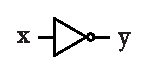
\includegraphics{not.eps}&
\begin{tabular}{c|c}
$x$ & $y$\\
\hline
$0$ & $1$\\
$1$ & $0$
\end{tabular}\\
(a) & (b) & (c)
\end{tabular}	
\caption{Logični izraz (a), logični simbol (b) in pravilnostna tabela (c) za negacijo.}
\label{fig:not}
\end{center}
\end{figure}


\subsection{Peircov operator}

Peircov operator (NE ALI, NOR) predstavlja invertirano (negirano) disjunkcijo. Operator vrne logično 1, ko so na logično 0 postavljene vse vhodne spremenljivke. V logičnem izrazu ga označujemo s simbolom $\downarrow$. Slika \ref{fig:nor} podaja logični izraz (a), logični simbol (b) in pravilnostno tabelo (c) za Peircov operator z dvema vhodnima spremenljivkama.

\begin{figure}[ht]
\begin{center}
\begin{tabular}{ccc}
$y = x_1 \downarrow x_2  = \ol{\left( x_1 \vee x_2 \right)}$&

\includegraphics{nor.eps}&
\begin{tabular}{cc|c}
$x_1$ & $x_2$ & $y$\\
\hline
$0$ & $0$ & $1$\\
$0$ & $1$ & $0$\\
$1$ & $0$ & $0$\\
$1$ & $1$ & $0$
\end{tabular}\\
(a) & (b) & (c)
\end{tabular}	
\caption{Logični izraz (a), logični simbol (b) in pravilnostna tabela (c) za Peircov operator z dvema vhodnima spremenljivkama.}
\label{fig:nor}
\end{center}
\end{figure}

Opozorilo: asociativnost za Peircov operator ne velja: $x_1 \downarrow x_2 \downarrow x_3 \neq \left( x_1 \downarrow x_2 \right) \downarrow x_3 \neq x_1 \downarrow \left(x_2 \downarrow x_3\right)$!

\subsection{Shefferjev operator}
Shefferjev operator (NE IN, NAND) predstavlja invertirano (negirano) konjunkcijo. Operator vrne logično 0, ko so na logično 1 postavljene vse vhodne spremenljivke. V logičnem izrazu ga označujemo s simbolom $\uparrow$. Slika \ref{fig:nor} podaja logični izraz (a), logični simbol (b) in pravilnostno tabelo (c) za Shefferjev operator z dvema vhodnima spremenljivkama.

\begin{figure}[ht]
\begin{center}
\begin{tabular}{ccc}
$y = x_1 \uparrow x_2 = \ol{\left( x_1 x_2 \right)}$&

\includegraphics{nand.eps}&
\begin{tabular}{cc|c}
$x_1$ & $x_2$ & $y$\\
\hline
$0$ & $0$ & $1$\\
$0$ & $1$ & $1$\\
$1$ & $0$ & $1$\\
$1$ & $1$ & $0$
\end{tabular}\\
(a) & (b) & (c)
\end{tabular}	
\caption{Logični izraz (a), logični simbol (b) in pravilnostna tabela (c) za Shefferjev operator z dvema vhodnima spremenljivkama.}
\label{fig:nand}
\end{center}
\end{figure}

Opozorilo: asociativnost za Shefferjev operator ne velja: $x_1 \uparrow x_2 \uparrow x_3 \neq \left( x_1 \uparrow x_2 \right) \uparrow x_3 \neq x_1 \uparrow \left(x_2 \uparrow x_3\right)$!

\subsection{Ekskluzivni ali}
Ekskluzivni ali (XOR, tudi vsota po modulu 2) dveh vhodnih spremenljivk vrne logično 1, ko logično vrednost 1 ekskluzivno zavzema ena vhodna spremenljivka. Pri več vhodnih spremenljivkah funkcija vrne logično 1, ko je na logično vrednost 1 postavljenih liho število vhodnih spremenljivk, kar si lahko interpretiramo tudi kot vsota po modulu 2 (opozorilo: v Logisimu XOR privzeto ne deluje na tak način -- pod lastnostmi XOR vrat moramo nastaviti polje \emph{Multiple-Input Behavior} na vrednost \emph{When an odd number are on}). V logičnem izrazu ekskluzivni ALI označujemo s simbolom $\nabla$ ali $\oplus$. Slika \ref{fig:xor} podaja logični izraz (a), logični simbol (b) in pravilnostno tabelo (c) za ekskluzivni ali z dvema vhodnima spremenljivkama.

\begin{figure}[ht]
\begin{center}
\begin{tabular}{ccc}
$y = x_1 \nabla x_2 =  \ol x_1 x_2 \vee x_1 \ol x_2$&

\includegraphics{xor.eps}&
\begin{tabular}{cc|c}
$x_1$ & $x_2$ & $y$\\
\hline
$0$ & $0$ & $0$\\
$0$ & $1$ & $1$\\
$1$ & $0$ & $1$\\
$1$ & $1$ & $0$
\end{tabular}\\
(a) & (b) & (c)
\end{tabular}	
\caption{Logični izraz (a), logični simbol (b) in pravilnostna tabela (c) za ekskluzivni ali z dvema vhodnima spremenljivkama.}
\label{fig:xor}
\end{center}
\end{figure}

\subsection{Ekvivalenca}
Ekvivalenca (XNOR) dveh vhodnih spremenljivk vrne logično 1, ko sta vhoda enaka in je tako enaka negiranemu ekskluzivnemu ali. Enakost pa ne velja za več vhodnih spremenljivk. V logičnem izrazu ekvivalenco označujemo s simbolom $\equiv$. Slika \ref{fig:xnor} podaja logični izraz (a), logični simbol (b) in pravilnostno tabelo (c) za ekvivalenco z dvema vhodnima spremenljivkama.

\begin{figure}[ht]
\begin{center}
\begin{tabular}{ccc}
$y = x_1 \equiv x_2 = \ol x_1 \ol x_2 \vee x_1 x_2$&

\includegraphics{xnor.eps}&
\begin{tabular}{cc|c}
$x_1$ & $x_2$ & $y$\\
\hline
$0$ & $0$ & $1$\\
$0$ & $1$ & $0$\\
$1$ & $0$ & $0$\\
$1$ & $1$ & $1$
\end{tabular}\\
(a) & (b) & (c)
\end{tabular}	
\caption{Logični izraz (a), logični simbol (b) in pravilnostna tabela (c) za ekvivalenco z dvema vhodnima spremenljivkama.}
\label{fig:xnor}
\end{center}
\end{figure}

\subsection{Implikacija }

Implikacija (IMP) dveh vhodnih spremenljivk, tj. $x_1 \rightarrow x_2$  vrne logično 0 le v primeru, da je operand na levi strani (tj. $x_1$) enak 1, operator na desni strani (tj. $x_2$) pa enak 0. Implikacija nima elektronske implementacije znotraj družine 7400. Prav tako operator nima logičnega simbola. Slika \ref{fig:imp} podaja logični izraz (a), in pravilnostno tabelo (b) za implikacijo.

\begin{figure}[ht]
\begin{center}
\begin{tabular}{cc}
$y = x_1 \rightarrow x_2 = \ol x_1 \vee x_2$&
\begin{tabular}{cc|c}
$x_1$ & $x_2$ & $y$\\
\hline
$0$ & $0$ & $1$\\
$0$ & $1$ & $1$\\
$1$ & $0$ & $0$\\
$1$ & $1$ & $1$
\end{tabular}\\
(a) & (b) 
\end{tabular}	
\caption{Logični izraz (a) in pravilnostna tabela (b) za implikacijo.}
\label{fig:imp}
\end{center}
\end{figure}

Opozorilo: komutativnost za implikacijo ali ne velja: $x_1 \rightarrow x_2 \neq x_2 \rightarrow x_1$!


\section{Analitično reševanje preklopnih funkcij}

Pri analitičnemu reševanju preklopnih funkcij preko postulatov in lastnosti Boolove algebre funkcijo podano z logičnim izrazom preoblikujemo v želeno obliko. Kadar želimo določeno lastnost formalno dokazati, se moramo pri spreminjanju oblike analitičnega izraza striktno držati postulatov Boolove algebre, pri čemer uporabimo le en postulat naenkrat, pri vsakem koraku izpeljave pa pripišemo postulat, ki smo ga uporabili. 

%\begin{zgled}
%Z uporabo postulatov Boolove algebre poenostavi izraz $xy(z \vee \ol y) \vee x \ol y$.	
%\end{zgled}
%\begin{resitev}
%\begin{align*}
%& xy(z \vee \ol y) \vee x \ol y  & \qquad (P4^*) \\
% = & xyz \vee xy \ol y \vee x \ol y & \qquad (P5^*) \\
% = & xyz \vee x0 \vee x \ol y & \qquad (P4^*) \\
% = & xyz \vee x(0 \vee \ol y) & \qquad (P3) \\
% = & xyz \vee x(\ol y \vee 0) & \qquad (P2) \\
% = & xyz \vee x \ol y
%\end{align*}
%\end{resitev}

\begin{zgled}
Z uporabo postulatov dokaži enakost $x \vee x = x$!
\end{zgled}

\begin{resitev}
\begin{align*}
& x \vee x = (x \vee x) \cdot 1  & \qquad (P2^*) \\
 = & (x \vee x) \cdot (x \vee \ol x) & \qquad (P5) \\
 = & x \vee (x \cdot \ol x)& \qquad (P4^*) \\
 = & x \vee 0 & \qquad (P5^*) \\
 = & x\qquad & (P2)
\end{align*}
\end{resitev}

Navadno pri poenostavljanju izrazov korake izpuščamo in nad izrazom neposredno uporabljamo lastnosti, ki sledijo iz postulatov. Če naloga od nas eksplicitno ne zahteva uporabe postulatov, jo rešujemo na tak način. Ker so postulati in lastnosti definirani nad osnovnimi logičnimi operatorji (konjunkcija, disjunkcija in negacija), vse funkcije v izrazu najprej izrazimo s temi.

\begin{zgled}
Poenostavi izraz $x_2 \rightarrow \left( \ol{\left( x_1 \vee \ol x_3 \right) \left( \ol x_1 \vee \ol x_3\right)}\right)$!
\end{zgled}
\begin{resitev}
\begin{align*}
&  x_2 \rightarrow \ol{\left( x_1 \vee \ol x_3 \right) \left( \ol x_1 \vee \ol x_3\right)}\\
 = & \ol x_2 \vee \ol{\left( x_1 \vee \ol x_3 \right) \left( \ol x_1 \vee \ol x_3\right)}\\
 = & \ol x_2 \vee \ol{\left( x_1 \vee \ol x_3 \right)} \vee \ol{\left( \ol x_1 \vee \ol x_3\right)}\\
 = & \ol x_2 \vee \ol x_1 x_3 \vee x_1 x_3\\
 = & \ol x_2 \vee (\ol x_1 \vee x_1) x_3\\
 = & \ol x_2 \vee x_3
\end{align*}
\end{resitev}




%\section{Logisim}
%\begin{itemize}
%\item Spletna stran, kjer lahko brezplačno snamemo program: http://ozark.hendrix.edu/~burch/logisim/
%\item Vrata in konfiguracija vrat.
%\item Vhodi in izhodi.
%\item Povezovanje.
%\item Simulacija.
%\end{itemize}

%Delo s protoboardi:
%\begin{itemize}
%\item Vrata vgrajena v čip, oznaka čipov, shema čipov, branje sheme.
%\item Vstavljanje čipa na protoboard in povezovanje priključkov (Opozorilo: pravilna lega čipa in priključitev napetosti!).
%\item Stikala in indikatorji.
%\item Napetost priključimo šele, ko je vezje dokončano in preverjeno.
%\item Iskanje napak s pomočjo indikatorja.
%\end{itemize}

%\section*{Laboratorijske vaje}
%\begin{figure}[ht]
%\centering
%\includegraphics[width=0.5\linewidth]{slika_v1.eps}
%\end{figure}

%\begin{itemize}
%\item Realiziraj zgornjo shemo v programu Logisim. S pomočjo simulacije vezja zapiši pravilnostno tabelo.
%\item Na protoborad priključi AND vrata in preveri pravilnost delovanja.
%\item Na protoboardu realiziraj zgornje vezje ter s pomočjo pravilnostne tabele ugotovi pravilnost delovanja vezja.
%\end{itemize}



\chapter{Priprava na 2. laboratorijske vaje}

\section{Zapis preklopnih funkcij}

%Za $n$ vhodnih spremenljivk obstaja $2^{2^n}$ preklopnih funkcij. Preklopno funkcijo lahko podamo na štiri načine:
%\begin{enumerate}
%\item tabelarični zapis (pravilnostna tabela),
%\item analitični zapis (z logičnim izrazom),
%\item matrični zapis (Veitchevi diagrami),
%\item logična shema (grafično).
%\end{enumerate}

Analitični zapis podajamo z logičnim izrazom oziroma logično enačbo. Pogosto se uporabljajo tri posebne oblike analitičnega zapisa, in sicer normalna, popolna in minimalna. Preklopna funkcija je podana v normalni obliki, če je sestavljena iz največ dveh nivojev logičnih operatorjev. Oblika je popolna, če na prvem nivoju logičnih operatorjev v vseh izrazih nastopajo vse vhodne spremenljivke. Minimalna oblika je najkrajša možna oblika zapisa preklopne funkcije.

\section{Analitični zapis in popolne normalne oblike zapisa preklopnih funkcij}

Pogledali si bomo popolno disjunktivno normalno obliko (PDNO) in popolno konjunktivno normalno obliko (PKNO) zapisa preklopne funkcije.

\subsection{Popolna disjunktivna normalna oblika (PDNO)}
\begin{itemize}
\item Disjunktivna: operator 2. nivoja je disjunkcija ($\vee$).
\item $f(x_1,x_2,...,x_n)=\vee_{i=0}^{2^{n}-1}m_i f(\vec{w}_i)$
\item $f(\vec{w}_i)$ ... vrednost funkcije pri $i$-tem vhodnem vektorju (vrstici)
\item minterm je konjunktiven izraz - vse vhodne spremenljivke so povezane preko konjunkcije
\item $m_i$ ... minterm $i$; $m_i = x_1^{w_{1,i}} \cdot x_2^{w_{2,i}} \cdot ... \cdot x_n^{w_{n,i}}; i=0,1,2,...,2^n-1$
\item $x^w = \left\{\begin{array}{clcr}
 x, w=1 \\ \ol x, w=0 \end{array} \right.$
\item $w_{j,i}$...$j$-ti bit binarnega zapisa števila $i$
\item PDNO lahko zapišemo v krajši obliki kot $f(x_1,x_2,...,x_n)=\vee^n(i_1,i_2,...,i_k)$, kjer $i_1,i_2,...,i_k$ določajo indekse mintermov, ki nastopajo v PDNO.
\end{itemize}

Recept: pri določanju PDNO disjunktivno vežemo tiste minterme, pri katerih je funkcijska vrednost 1. Pri tem se $i$-ti minterm nanaša na funkcijsko vrednost $f(\vec{w}_i)$ (glej tabelo \ref{tab:mintermi}).

\begin{table}[ht]
\centering
\begin{tabular}{ccc|c|c}
$x_1$ & $x_2$ & $x_3$ & f($x_1$,$x_2$,$x_3$) & minterm\\
\hline
0 & 0 & 0 & $f(\vec{w}_0)$ & $m_0$ \\
0 & 0 & 1 & $f(\vec{w}_1)$ & $m_1$ \\
0 & 1 & 0 & $f(\vec{w}_2)$ & $m_2$ \\
0 & 1 & 1 & $f(\vec{w}_3)$ & $m_3$ \\
1 & 0 & 0 & $f(\vec{w}_4)$ & $m_4$ \\
1 & 0 & 1 & $f(\vec{w}_5)$ & $m_5$ \\
1 & 1 & 0 & $f(\vec{w}_6)$ & $m_6$ \\
1 & 1 & 1 & $f(\vec{w}_7)$ & $m_7$ 
\end{tabular}
\caption{Primer pravilnostne tabele in zaporedja mintermov za preklopno funkcijo treh vhodnih spremenljivk.}
\label{tab:mintermi}
\end{table}

\begin{zgled}
Zapiši minterm 9, pri 4-ih vhodnih spremenljivkah:
\end{zgled}

\begin{resitev}
Velja torej:
\begin{itemize}
\item $n=4$,
\item $i = 9_{[10]} = 1001_{[2]}$,
\item $m_9 = x_1^1 x_2^0 x_3^0 x_4^1 = x_1 \ol x_2 \ol x_3 x_4$.
\end{itemize}
\end{resitev}

\subsection{Popolna konjunktivna normalna oblika (PKNO)}
\begin{itemize}
\item Konjunktivna: operator 2. nivoja je konjunkcija ($\&$).
\item $f(x_1,x_2,...,x_n)=\&_{i=0}^{2^{n}-1}\left( M_{2^{n}-1-i} \vee f(\vec{w}_i)\right)$
\item maksterm je disjunktiven izraz - vhodne spremenljivke so povezane preko disjunkcije
\item $M_{2^{n}-1-i}$ ... maksterm $2^{n}-1-i$; $M_{2^{n}-1-i} = x_1^{\ol w_{1,i}} \vee x_2^{\ol w_{2,i}} \vee ... \vee x_n^{\ol w_{n,i}}; i=0,1,2,...,2^n-1$
\item PKNO lahko zapišemo v krajši obliki: $f(x_1,x_2,...,x_n)=\&^n(i_m,i_{m-1},...,i_1)$, kjer $i_m,i_{m-1},...,i_1$ določajo indekse makstermov, ki nastopajo v PKNO.
\end{itemize}

Recept: pri določanju PKNO konjunktivno vežemo tiste maksterme, pri katerih je funkcijska vrednost 0. Pri tem se $(2^n-1-i)$-ti maksterm nanaša na funkcijsko vrednost $f(\vec{w}_i)$ (glej tabelo \ref{tab:makstermi}).


\begin{table}[ht]
\centering
\begin{tabular}{ccc|c|c}
$x_1$ & $x_2$ & $x_3$ & f($x_1$,$x_2$,$x_3$) & maksterm\\
\hline
0 & 0 & 0 & $f(\vec{w}_0)$ & $M_7$ \\
0 & 0 & 1 & $f(\vec{w}_1)$ & $M_6$ \\
0 & 1 & 0 & $f(\vec{w}_2)$ & $M_5$ \\
0 & 1 & 1 & $f(\vec{w}_3)$ & $M_4$ \\
1 & 0 & 0 & $f(\vec{w}_4)$ & $M_3$ \\
1 & 0 & 1 & $f(\vec{w}_5)$ & $M_2$ \\
1 & 1 & 0 & $f(\vec{w}_6)$ & $M_1$ \\
1 & 1 & 1 & $f(\vec{w}_7)$ & $M_0$ \\
\end{tabular}
\caption{Primer pravilnostne tabele in zaporedja makstermov za preklopno funkcijo treh vhodnih spremenljivk.}
\label{tab:makstermi}
\end{table}

\begin{zgled}
Zapiši maksterm 9 pri 4-ih vhodnih spremenljivkah.
\end{zgled}
\begin{resitev}
Velja torej:
\begin{itemize}
\item $n=4$,
\item $i = 2^n-1 - 9=15-9=6$,
\item $6_{[10]} = 0110_{[2]}$,
\item $M_9 = x_1^{\ol 0} \vee x_2^{\ol 1} \vee x_3^{\ol 1} \vee x_4^{\ol 0} = x_1 \vee \ol x_2 \vee \ol x_3 \vee x_4$.
\end{itemize}
\end{resitev}

\begin{zgled}
Podano funkcijo pretvori v popolno disjunktivno normalno obliko na dva načina:
\begin{itemize}
\item{s pomočjo pravilnostne tabele},
\item{analitično z razširitvijo}.
\end{itemize}
\end{zgled}
\begin{resitev}
Funkcija:
$$
f(x_1,x_2,x_3) = x_1 \vee x_1 \ol x_2 \vee \ol x_2 \ol x_3
$$
je že zapisana v \textit{disjunktivni normalni obliki}, ki pa ni popolna. 

\bigskip

\textbf{Pretvorba s pomočjo pravilnostne tabele}

Zapišimo pravilnostno tabelo, s pomočjo katere lahko zapišemo PDNO, tako da prepišemo tiste minterme, pri katerih je vrednost funkcije enaka 1.\\
\begin{table}[ht]
\centering
\begin{tabular}{ccc|c|c|c}
$x_1$ & $x_2$ & $x_3$ & f($x_1$,$x_2$,$x_3$) & minterm & maksterm\\
\hline
0 & 0 & 0 & 1 & $m_0$ & $M_7$ \\
0 & 0 & 1 & 0 & $m_1$ & $M_6$ \\
0 & 1 & 0 & 0 & $m_2$ & $M_5$ \\
0 & 1 & 1 & 0 & $m_3$ & $M_4$ \\
1 & 0 & 0 & 1 & $m_4$ & $M_3$ \\
1 & 0 & 1 & 1 & $m_5$ & $M_2$ \\
1 & 1 & 0 & 1 & $m_6$ & $M_1$ \\
1 & 1 & 1 & 1 & $m_7$ & $M_0$ \\
\end{tabular}
\caption{Pravilnostna tabela funkcije $f(x_1,x_2,x_3) = x_1 \vee x_1 \ol x_2 \vee \ol x_2 \ol x_3$.}
\end{table}


Če izpišemo samo indekse teh mintermov, dobimo skrajšano obliko PDNO:\\
\hspace*{5mm} $f(x_1,x_2,x_3)=\vee^3(0,4,5,6,7)$. \\

\bigskip
Zapišimo PDNO še v eksplicitni obliki: \\
\hspace*{5mm} $f(x_1,x_2,x_3)=\ol x_1 \ol x_2 \ol x_3 \vee x_1 \ol x_2 \ol x_3 \vee x_1 \ol x_2 x_3 \vee x_1 x_2 \ol x_3 \vee x_1 x_2 x_3$. \\

\textbf{Analitična pretvorba z razširitvijo}

Funkcijo razširimo v popolno (na prvem nivoju morajo nastopati vse vhodne spremenljivke):
\begin{align*}
&x_1 \vee x_1 \ol x_2 \vee \ol x_2 \ol x_3 \\
= & x_1(x_2 \vee \ol x_2)(x_3 \vee \ol x_3) \vee x_1 \ol x_2 (x_3 \vee \ol x_3) \vee (x_1 \vee \ol x_1)\ol x_2 \ol x_3 \\
= & x_1 x_2 x_3 \vee x_1 x_2 \ol x_3 \vee x_1 \ol x_2 x_3 \vee x_1 \ol x_2 \ol x_3 \vee \hsout{x_1 \ol x_2 x_3} \vee \hsout{x_1 \ol x_2 \ol x_3} \vee \hsout{x_1 \ol x_2 \ol x_3} \vee \ol x_1 \ol x_2 \ol x_3\\
= & x_1 x_2 x_3 \vee x_1 x_2 \ol x_3 \vee x_1 \ol x_2 x_3 \vee x_1 \ol x_2 \ol x_3 \vee \ol x_1 \ol x_2 \ol x_3 \\
= & \vee^3(7,6,5,4,0) \\
= & \vee^3(0,4,5,6,7) \\
\end{align*}

\end{resitev}

\subsection{Relaciji med makstermi in mintermi}
Med mintermi in makstermi zaradi DeMorganovega pravila veljata sledeči relaciji: 
\begin{itemize}
\item $\ol m_i = M_{2^n-1-i},$ 
\item $\ol M_i = m_{2^n-1-i}.$
\end{itemize}

Relaciji lahko uporabimo pri pretvarjanju funkcije iz PDNO v PKNO in obratno. Pri podanem zapisu najprej pogledamo kateri termi manjkajo:
\begin{itemize}
\item Če je funkcija podana v PDNO, izpišemo manjkajoče minterme - v pravilnostni tabeli so soležni z enicami.
\item Če je funkcija podana v PKNO, izpišemo manjkajoče maksterme - v pravilnostni tabeli so soležni z ničlami.
\end{itemize}
S tem smo dobili pozicije termov, ki nastopajo v iskani obliki zapisa preklopne funkcije. Indekse iskanih termov dobimo tako, da nad izpisanimi mintermi oziroma makstermi uporabimo zgoraj navedeni relaciji.

\subsection{Pretvarjanje med PDNO in PKNO}
Dva možna načina reševanja:
\begin{enumerate}
\item zapišemo pravilnostno tabelo in iz nje razberemo rešitev,
\item z upoštevanjem relacij med mintermi in makstermi.
\end{enumerate}

\begin{zgled}
Funkcijo podano v PDNO pretvori v PKNO:
\begin{itemize}
\item s pomočjo pravilnostne tabele,
\item z upoštevanjem relacij med mintermi in makstermi.
\end{itemize}
\end{zgled}
\begin{resitev}
Demonstrirajmo oba načina pretvorbe.

\textbf{Pretvorba iz PDNO v PKNO: s pomočjo pravilnostne tabele} \\
Glej tabelo v prejšnjem zgledu!

Prepišemo maksterme, pri katerih je vrednost funkcije enaka 0.

\hspace*{5mm} PKNO: $\&^3(6,5,4)$

Eksplicitna PKNO: \\
\hspace*{5mm} PKNO: $(x_1 \vee x_2 \vee \ol x_3) (x_1 \vee \ol x_2 \vee x_3) (x_1 \vee \ol x_2 \vee \ol x_3)$.\\

\textbf{Pretvorba iz PDNO v PKNO: z upoštevanjem relacij med mintermi in makstermi}

Pretvorimo $\vee^3(0,4,5,6,7)$ v PKNO:
\begin{enumerate}
\item zapišemo manjkajoče minterme: $m_1,m_2,m_3$.
\item izračunamo indekse makstermov: $M_6, M_5, M_4$.
\item rešitev: $\&^3(6,5,4)$.
\end{enumerate}

Na podoben način, bi lahko pretvarjali tudi iz PKNO v PDNO.

\end{resitev}


%\section*{Laboratorijske vaje}
%S programom \textit{Logisim} realiziraj preklopno funkcijo
%$$
%f(x_1,x_2,x_3) = \&^3(6,4,1,0)
%$$
%in s simulacijo preveri pravilnost sheme.
%
%\bigskip
%Eksplicitna 
%Minimalna oblika: $f(x_1,x_2,x_3) = \ol x_1 \ol x_3 \vee x_1 \ol x_2$.\\
%Pravilnostna tabela: \\
%\begin{table}[ht]
%\centering
%\begin{tabular}{ccc|c}
%$x_1$ & $x_2$ & $x_3$ & f($x_1$,$x_2$,$x_3$) \\
%\hline
%0 & 0 & 0 & 1 \\
%0 & 0 & 1 & 0 \\
%0 & 1 & 0 & 1 \\
%0 & 1 & 1 & 0 \\
%1 & 0 & 0 & 1 \\
%1 & 0 & 1 & 1 \\
%1 & 1 & 0 & 0 \\
%1 & 1 & 1 & 0 \\
%\end{tabular}
%\end{table}
%
%Shema:\\
%\begin{figure}[ht]
%\centering
%\includegraphics[width=0.5\linewidth]{slika_v2_2.eps}
%\end{figure}
%\end{itemize}

%\subsection*{Popolna konjunktivna normalna oblika (PKNO)}
%\begin{itemize}
%\item Konjunktivna: operator 2. nivoja je konjunkcija($ \&$).
%\item $f(x_1,x_2,...,x_n)=\&_0^{2^{n}-1} \left( M_{2^{n}-1-i} \vee f(\vec{w}_i) \right)$

\chapter{Priprava na 3. laboratorijske vaje}

\section{Zapis preklopnih funkcij z Veitchevim diagramom}

Veitchevi diagrami igrajo pomembno vlogo pri minimizaciji preklopnih funkcij. Veitchev diagram pri $n$ vhodnih spremenljivkah je sestavljen iz $2^n$ polj, pri čemer posamezno polje vsebuje funkcijsko vrednost pri posameznem mintermu. Postopek zapisovanja Veitchevega diagrama je razmeroma preprost, in sicer izhajamo iz diagrama za eno spremenljivko (glej sliko \ref{fig:Veitch}(a)). Diagram za dve spremenljivki dobimo tako, da podvojimo diagram za eno spremenljivko. Označiti je potrebno tudi pokritja, in sicer tako, da posamezna spremenljivka pokriva polovico Veitchevega diagrama. Pokritja lahko izbiramo na različne načine. V splošnem dobimo diagram za $n$ spremenljivk tako, da podvojimo diagram za $n-1$ spremenljivk in na novo dodani del pokrijemo z dodano spremenljivko.

\begin{figure}[ht]
\begin{center}
	\begin{tabular}{ccc}
		
\includegraphics{veitch-1.eps} & 
\includegraphics{veitch-2.eps} & 
\includegraphics{veitch-3.eps}\\
		(a) & (b) & (c)\\
	\end{tabular}		
	\begin{tabular}{cc}
		
\includegraphics{veitch-4.eps} & 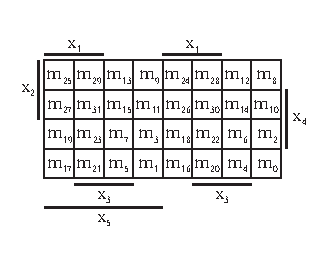
\includegraphics{veitch-5.eps}\\
		(d) & (e)\\
	\end{tabular}	
	
\end{center}
\caption{Slika (a) prikazuje Veitchev diagram za eno vhodno spremenljivko, slika (b) za dve, slika (c) za tri, slika (d) za štiri, slika (e) pa za pet.}
\label{fig:Veitch}
\end{figure}

\begin{zgled}
Funkcijo $f(x_1,x_2,x_3,x_4) = \vee^4(5, 7, 9, 11, 13, 15)$ zapiši v Veitchev diagram. 
\end{zgled}
\begin{resitev}
V polja, ki se nanašajo na minterme, pri katerih je funkcijska vrednost enaka 1, vpišemo enice, ostala polja pa pustimo prazna (glej sliko \ref{fig:Veitch-zgled}).

\begin{figure}[ht]
\begin{center}
	
\includegraphics{veitch-zgled.eps} 
\end{center}
\caption{Veitchev diagram funkcije $f(x_1,x_2,x_3,x_4) = \vee^4(5, 7, 9, 11, 13, 15)$.}
\label{fig:Veitch-zgled}
\end{figure}

\end{resitev}

\section{Funkcijsko poln sistem}

Funkcijsko poln sistem je nabor logičnih funkcij, s katerimi lahko izrazimo katerokoli logično funkcijo. Iz definicije Boolove algebre sledi, da je $\{\vee,\cdot,\neg\}$ funkcijsko poln sistem (operator $\neg\ $ predstavlja negacijo).

Funkcijsko polnost ugotavljamo na dva načina:
\begin{itemize}
\item s pretvorbo na nek znan funkcijsko poln sistem,
\item s preverjanjem pripadnosti osnovnim zaprtim razredom.
\end{itemize}

\begin{zgled}
S pretvorbo na negacijo, konjunkcijo in disjunkcijo pokaži, da je Shefferjev operator funkcijsko poln sistem.
\end{zgled}
\begin{resitev}

S Shefferjevim operatorjem izrazimo negacijo.

\begin{align*}
\ol x & = \ol x \ol x  = x \uparrow x\\
\end{align*}
S Shefferjevim operatorjem izrazimo konjunkcijo.
\begin{align*}
x_1 x_2 & = \ol{\ol{x_1 x_2}} = \ol{x_1 \uparrow x_2} = (x_1 \uparrow x_2) \uparrow (x_1 \uparrow x_2) \\
\end{align*}
S Shefferjevim operatorjem izrazimo disjunkcijo.
\begin{align*}
x_1 \vee x_2 & = \ol{\ol{x_1 \vee x_2}} = \ol{\ol x_1 \ol x_2} = (x_1 \uparrow x_1) \uparrow (x_2 \uparrow x_2)
\end{align*}
\end{resitev}
Podobno bi se dalo pokazati za Peircov operator.



\chapter{Priprava na 4. laboratorijske vaje}

\section{Zaprti razredi in preverjanje funkcijske polnosti sistema}
%Naj bo $P_n$ množica vseh preklopnih funkcij nad $n$ vhodnimi spremenljivkami in naj bo $M \subset P_n$ njena podmnožica. Naj bo $f \in M$ poljubna funkcija. Če z $f$ ne moremo izraziti nobene funkcije $g \notin M$, je $M$ zaprt razred.

Funkcijo polnost nabora logičnih funkcij lahko preverjamo s pripadnostjo nabora osnovnim zaprtim razredom logičnih funkcij (Postov teorem funkcijske polnosti). Osnovni zaprti razredi so sledeči:
\begin{itemize}
%\item $P_n$ -- univerzalna množica
\item $T_0$ -- razred preklopnih funkcij, ki ohranjajo ničlo ($f(0,0,\ldots,0) = 0$)
\item $T_1$ -- razred preklopnih funkcij, ki ohranjajo enico ($f(1,1,\ldots,1) = 1$)
\item $S$ -- razred sebidualnih funkcij ($\ol f (\ol x_1,\ol x_2,\ldots,\ol x_n) = f(x_1,x_2,\ldots,x_n)$)
\item $L$ -- razred linearnih funkcij ($f(x_1, x_2,...,x_n) \in L$, $f(x_1,x_2,...,x_n)$ $=$ \\= $a_0 \nabla a_1 x_2 \nabla ... \nabla a_n x_n$)
\item $M$ -- razred monotonih funkcij ($f(x_1, x_2,...,x_n) \in M, \forall i,j: $ \\$\vec{w}_i < \vec{w}_j \rightarrow f(\vec{w}_i) \leq f(\vec{w}_j)$)
\end{itemize}
Če nabor odpira vse osnovne razrede, je poln. Nabor odpira nek osnovni razred, če vsaj ena izmed funkcij v podanem naboru ne pripada izbranemu razredu. 


\begin{zgled}
S pomočjo zaprtih razredov preveri funkcijsko polnost nabora $\{\vee,\rightarrow,1\}$.
\end{zgled}
\begin{resitev}
Cilj: Pri vsakem osnovnem razredu želimo najti vsaj eno funkcijo iz podanega nabora, ki temu razredu ne pripada.

\begin{enumerate}
\item Razred $T_0$:
\begin{itemize}
\item $\vee: f(0,0) = 0 \vee 0 = 0$; pripada razredu.
\item $1: 1 \neq 0$; ne pripada razredu.
\end{itemize}

\item Razred $T_1$:
\begin{itemize}
\item $\vee: f(1,1) = 1 \vee 1 = 1$; pripada razredu.
\item $\rightarrow: f(1,1) = 1 \rightarrow 1 = 1$; pripada razredu.
\item $1: 1 = 1$; pripada razredu
\end{itemize}
Nabor $\{\vee,\rightarrow,1\}$ ne odpira razreda $T_1$, torej nabor ni poln. Vseeno nadaljujmo s postopkom.

\item Razred $S$:

Pripadnost lahko dokazujemo na dva načina:
\begin{itemize}
\item analitično: ali velja $f(x_1,x_2,...,x_n) = \ol f(\ol x_1, \ol x_2,...,\ol x_n)$,
\item tabelarično: ali velja $f(\vec{w}_i) \neq f(\vec{w}_{2^n-1-i})$.
\end{itemize}

Postopek:
\begin{itemize}
\item $1:$ (analitično)\\
\begin{align*}
\ol 1 & = 1\\
0 & = 1 \quad \text{protislovje}
\end{align*}
Funkcija ne pripada razredu $S$. Vseeno nadaljujmo.

\item $\vee:$ (analitično)\\
\begin{align*}
\ol f (\ol x_1, \ol x_2) & = f(x_1,x_2)\\
\ol{\ol x_1 \vee \ol x_2} & = x_1 \vee x_2 \quad \text{(desno stran dopolnimo do PDNO)} \\
x_1 x_2 & = x_1(x_2 \vee \ol x_2) \vee x_2 (x_1 \vee \ol x_1)\\
x_1 x_2 & = x_1 x_2 \vee x_1 \ol x_2 \vee x_1 x_2 \vee \ol x_1 x_2\\
x_1 x_2 & = \ol x_1 x_2 \vee x_1 \ol x_2 \vee x_1 x_2\\
\vee^2(3) & \neq \vee^2(1,2,3) \qquad \rightarrow \vee \notin S
\end{align*}

\item $\rightarrow:$ (tabelarično)\\
\begin{table}[ht]
\centering
\begin{tabular}{cc|c}
$x_1$ & $x_2$ & $x_1 \rightarrow x_2$\\
\hline
0 & 0 & 1\\
0 & 1 & 1\\
\hline
1 & 0 & 0\\
1 & 1 & 1
\end{tabular}
\end{table}

$f(w_0) = f(w_3)$ -- funkcija ne pripada $S$.
\end{itemize}

\item Razred $L:$\\
Funkcija $f(x_1,x_2,\ldots,x_n)$ spada v razred linearnih funkcij, če jo lahko zapišemo kot
$$
f(x_1,x_2,\ldots,x_n) = a_0 \nabla a_1 x_1 \nabla a_2 x_2 \nabla \cdots \nabla a_n x_n.
$$
Pripadnost lahko preverjamo:
\begin{itemize}
\item analitično,
\item z Veitchevim diagramom.
\end{itemize}

Analitično preverjanje:
\begin{itemize}
\item predpostavimo, da funkcija $f(x_1,x_2,\ldots,x_n)$ spada v razred linearnih funkcij,
\item določimo koeficiente $a_0,a_1,\cdots,a_n$,
\item preverimo, če se dobljena funkcija $a_0 \nabla a_1 x_1 \nabla a_2 x_2 \nabla \cdots \nabla a_n x_n$ ujema s podano funkcijo $f(x_1,x_2,\ldots,x_n)$.
\end{itemize}

Postopek:
\begin{itemize}
\item $\vee:$\\
Predpostavimo, da je disjunkcija linearna funkcija, tedaj jo lahko zapišemo kot:
\begin{align*}
f(x_1,x_2)_L & = x_1 \vee x_2 = a_0 \nabla a_1 x_1 \nabla a_2 x_2\\
\hspace{5mm}\\
f(0,0)_L & = a_0 \nabla a_1 0 \nabla a_2 0 = a_0 = 0 \nabla 0 = 0 \quad (a_0 = 0)\\
f(0,1)_L & = 0 \nabla a_1 0 \nabla a_2 1 = a_2 = 0 \nabla 1 = 1 \quad (a_2 = 1)\\
f(1,0)_L & = 0 \nabla a_1 1 \nabla a_2 0 = a_1 = 1 \nabla 0 = 1 \quad (a_1 = 1)\\
f(x_1,x_2)_L &= 0 \nabla 1 x_1 \nabla 1 x_2 = x_1 \nabla x_2
\end{align*}
Preverimo za vse preostale vhodne vektorje (v primeru protislovja postopek ustavimo):
\begin{align*}
f(1,1) &= 1 \vee 1 = 1 \\
f(1,1)_L &= x_1 \nabla x_2 = 1 \nabla 1 = 0
\end{align*}
Protislovje. Funkcija ne pripada razredu.
\end{itemize}

Preverjanje z Veitchevim diagramom:
\begin{itemize}
\item Preklopna funkcija spada v razred $L$, če pri primerjavi pokritij velja popolna enakost ali popolna različnost vrednosti funkcije.
\end{itemize}

Postopek:
\begin{itemize}
\item $\vee:$\\
Preverimo pokritja:
\begin{figure}[!htb]
	\centering
	
\includegraphics{veitch_OR.eps}
	\label{f1}
\end{figure}

\begin{itemize}
\item $\ol x_1 x_2 : \ol x_1 \ol x_2$ (popolnoma različna), \\
\item $x_1 : \ol x_1$ (niti popolnoma različna niti popolnoma enaka).
\end{itemize}
Funkcija ne pripada razredu.
\end{itemize}

\item Razred $M$:
Funkcija pripada $M$, če pri vseh vhodnih vektorjih velja, da je pri manjšem vektorju vrednost funkcije manjša ali enaka vrednosti pri večjem vektorju. Relacija \emph{je manjši} je definirana na sledeči način:
\begin{itemize}
\item Za vhodna vektorja $w_i$ in $w_j$ velja $w_i < w_j$, če za vsako mesto $k$ velja $w_{k,i} \leq w_{k,j}$. Primer: $(1,0,0,1,0,1,0,0) < (1,1,0,1,0,1,0,1)$.
\end{itemize}
Pri preverjanju pripadnosti je dovolj, da preverimo le sosedne vhodne vektorje. Vhodna vektorja sta sosedna, če se razlikujeta le na enem mestu. Primer: $(1,0,0,1,0)$ in $(1,0,1,1,0)$.

Postopek:
\begin{itemize}
\item $\rightarrow:$\\
\begin{table}[ht]
\centering
\begin{tabular}{cc|c}
$x_1$ & $x_2$ & $x_1 \rightarrow x_2$\\
\hline
0 & 0 & 1\\
0 & 1 & 1\\
1 & 0 & 0\\
1 & 1 & 1
\end{tabular}
\end{table}

Preverjamo samo sosedne vektorje. Sosedni vhodni vektorji so $(w_0,w_1)$, $(w_0,w_2)$, $(w_1,w_3)$ in $(w_2,w_3)$. Hitro najdemo protislovje, in sicer $w_0 < w_2, f(w_0) > f(w_2)$. Funkcija torej ne pripada $M$.
\end{itemize}
\end{enumerate}
\end{resitev}

\begin{zgled}
Analitično preveri ali preklopna funkcija $f(x_1,x_2,x_3,x_4)=\&^4(0,1,6,8,9,14)$ pripada razredu linearnih funkcij.\\
\end{zgled}
\begin{resitev}
Postopek:

\begin{table}[ht]
\centering
\begin{tabular}{cccc|c|c}
$x_1$ & $x_2$ & $x_3$ & $x_4$ & $f(x_1,x_2,x_3,x_4)$ & $f(x_1,x_2,x_3,x_4)_L$\\
\hline
0 & 0 & 0 & 0 & 1 & 1\\
0 & 0 & 0 & 1 & 0 & 0\\
0 & 0 & 1 & 0 & 1 & 1\\
0 & 0 & 1 & 1 & 1 & 0\\
0 & 1 & 0 & 0 & 1 & 1\\
0 & 1 & 0 & 1 & 1 & 0\\
0 & 1 & 1 & 0 & 0 & 1\\
0 & 1 & 1 & 1 & 0 & 0\\
1 & 0 & 0 & 0 & 1 & 1\\
1 & 0 & 0 & 1 & 0 & 0\\
1 & 0 & 1 & 0 & 1 & 1\\
1 & 0 & 1 & 1 & 1 & 0\\
1 & 1 & 0 & 0 & 1 & 1\\
1 & 1 & 0 & 1 & 1 & 0\\
1 & 1 & 1 & 0 & 0 & 1\\
1 & 1 & 1 & 1 & 0 & 0\\
\end{tabular}
\end{table}
Predpostavimo, da dana funkcija pripada razredu linearnih funkcij, tedaj jo lahko zapišemo kot:
\begin{align*}
f(x_1,x_2,x_3,x_4)_L & = a_0 \nabla a_1 x_1 \nabla a_2 x_2 \nabla a_3 x_3 \nabla a_4 x_4\\
\hspace{5mm}\\
f(0,0,0,0)_L & = a_0 \nabla a_1 0 \nabla a_2 0 \nabla a_3 0 \nabla a_4 0 = 1 \quad (a_0 = 1)\\
f(0,0,0,1)_L & = 1 \nabla a_1 0 \nabla a_2 0 \nabla a_3 0 \nabla a_4 1 = 1 \nabla a_4 = 0 \quad (a_4 = 1)\\
f(0,0,1,0)_L & = 1 \nabla a_1 0 \nabla a_2 0 \nabla a_3 1 \nabla a_4 0 = 1 \nabla a_3 = 1 \quad (a_3 = 0)\\
f(0,1,0,0)_L & = 1 \nabla a_1 0 \nabla a_2 1 \nabla a_3 0 \nabla a_4 0 = 1 \nabla a_2 = 1 \quad (a_2 = 0)\\
f(1,0,0,0)_L & = 1 \nabla a_1 1 \nabla a_2 0 \nabla a_3 0 \nabla a_4 0 = 1 \nabla a_1 = 1 \quad (a_1 = 0)\\
f(x_1,x_2, x_3, x_4)_L &= 1 \nabla 0 x_1 \nabla 0 x_2 \nabla 0 x_3 \nabla 1 x_4 = 1 \nabla x_4 = \ol x_4
\end{align*}
Preverimo za vse preostale vhodne vektorje (v primeru protislovja postopek ustavimo):
\begin{align*}
f(0,0,1,1) &= 1 \\
f(0,0,1,1)_L &= 1 \nabla 1 = 0
\end{align*}
Protislovje. Funkcija ne pripada razredu.
\end{resitev}

\chapter{Priprava na 5. laboratorijske vaje}
\section{Minimalne oblike zapisa preklopnih funkcij}

Minimalna oblika zapisa preklopne funkcije podaja najkrajši možen zapis te funkcije. Poznamo več minimalnih oblik zapisa. Pogledali si bomo sledeče:
\begin{itemize}
\item minimalna disjunktivna normalna oblika (MDNO): določa najkrašo disjunktivno normalno obliko zapisa preklopne funkcije,
\item minimalna konjunktivna normalna oblika (MKNO): določa najkrašo konjunktivno normalno obliko zapisa preklopne funkcije,
\item minimalna normalna oblika (MNO): določa nakrajšo normalno obliko zapisa preklopne funkcije.
\end{itemize}

Pri določanju minimalne disjunktivne normalne oblike (MDNO) izhajamo iz iskanja \emph{glavnih vsebovalnikov}. Glavni vsebovalnik predstavlja najkrajši konjunktivni izraz, ki je skupen podmnožici mintermov, ki sestavljajo PDNO podane funkcije. Najmanjša množica glavnih vsebovalnikov, ki skupaj pokrijejo celotno množico mintermov v PDNO, predstavlja minimalno disjunktivno normalno obliko.\\

Pri določanju minimalne konjunktivne normalne oblike (MKNO) izhajamo iz določanja MDNO negirane funkcije, ki jo z uporabo DeMorganovega pravila pripeljemo do konjunktivne oblike.\\

Pri določanju minimalne normalne oblike (MNO) upoštevamo dejstvo, da MNO predstavlja krajšo izmed MDNO in MKNO.\\

Glavne vsebovalnike iščemo na podlagi \emph{sosednosti} med konjunktivni izrazi. Dva konjunktivna izraza sta sosedna, če se razlikujeta po natanko eni negaciji:
\begin{itemize}
\item izraza $x_{1}^{w_1} \cdot x_{2}^{w_2} \cdot ... \cdot x_{i}^{w_i} \cdot ... \cdot x_{n}^{w_n}$ in $x_{1}^{w_1} \cdot x_{2}^{w_2} \cdot ... \cdot x_{i}^{\ol w_i} \cdot ... \cdot x_{n}^{w_n}$ sta sosedna, ker se razlikujeta le po negaciji nad vhodno spremenljivko z indeksom $i$.
\end{itemize}
V splošnem velja, da ima izraz, ki vsebuje $n$ vhodnih spremenljivk, $n$ sosednih izrazov.

\begin{zgled}
Zapiši vse izraze, ki so sosedni izrazu $x_1 \ol x_2 x_4$.\\
\end{zgled}
\begin{resitev}
V sosednih izrazih nastopajo enake spremenljivke kot v izhodiščnem izrazu. Od izhodiščnega izraza se sosedni razlikujejo po natanko eni negaciji. Sosedni izrazi so torej:
\begin{itemize}
\item $\ol x_1 \ol x_2 x_4$,
\item $x_1 x_2 x_4$ in
\item $x_1 \ol x_2 \ol x_4$.
\end{itemize}

\end{resitev}

Glavni vsebovalnik dveh sosednih izrazov določimo z upoštevanjem lastnosti, da je disjunkcija dveh termov, ki se razlikujeta natanko po negaciji nad eno spremenljivko, neodvisna od vrednosti te spremenljivke. Glavni vsebovalnik dveh sosednih izrazov $x_{1}^{w_1} \cdot x_{2}^{w_2} \cdot ... \cdot x_{i-1}^{w_{i-1}} \cdot x_{i}^{w_i} \cdot x_{i+1}^{w_{i+1}} \cdot ... \cdot x_{n}^{w_n}$ in $x_{1}^{w_1} \cdot x_{2}^{w_2} \cdot ... \cdot x_{i-1}^{w_{i-1}} \cdot x_{i}^{\ol w_i} \cdot x_{i+1}^{w_{i+1}} \cdot ... \cdot x_{n}^{w_n}$ je torej izraz $x_{1}^{w_1} \cdot x_{2}^{w_2} \cdot ... \cdot x_{i-1}^{w_{i-1}} \cdot x_{i+1}^{w_{i+1}} \cdot ... \cdot x_{n}^{w_n}$. 

\begin{zgled}
Določi glavni vsebovalnik izrazov $\ol x_1 \ol x_2 \ol x_3 x_4$ in $x_1 \ol x_2 \ol x_3 x_4$.\\
\end{zgled}
\begin{resitev}
Izraza se razlikujeta le po negaciji nad spremenljivko $x_1$. Disjunkcija med izrazoma je torej neodvisna od vrednosti te spremenljivke, zato je njun glavni vsebovalnik $\ol x_2 \ol x_3 x_4$.

\end{resitev}



\section{Veitchev postopek minimizacije}
Veitchev postopek minimizacije izkorišča lastnosti Veitchevega diagrama. Sosednost mintermov je namreč neposredno povezana s sosednostjo celic v diagramu. Pri celicah, ki se nahajajo na robovih diagrama se sosednost prenaša na zrcalno stran (glej sliko \ref{fig:Veitch_sosednost}).

\begin{figure}[ht]
\begin{center}
	\begin{tabular}{ccc}
		
\includegraphics{veitch_sosednost-1.eps} & 
\includegraphics{veitch_sosednost-2.eps} & 
\includegraphics{veitch_sosednost-3.eps}\\
		(a) & (b) & (c)\\
	\end{tabular}		
	\begin{tabular}{cc}
		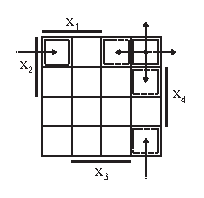
\includegraphics{veitch_sosednost-4.eps} & 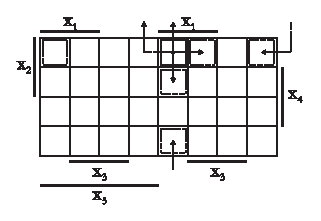
\includegraphics{veitch_sosednost-5.eps}\\
		(d) & (e)\\
	\end{tabular}	
	
\end{center}
\caption{Slika (a) prikazuje sosednost v Veitchevem diagramu za 1 vhodno spremenljivko, slika (b) za 2, slika (c) za 3, slika (d) za 4, slika (e) pa za 5.}
\label{fig:Veitch_sosednost}
\end{figure}

\begin{zgled}
V Veitchevem diagramu za 4 spremenljivke označi izraze, ki so sosednji izrazu $m_{14} \vee m_{15}$.\\
\end{zgled}
\begin{resitev}
Izraz zapišimo v razširjeni obliki: 
$$ m_{14} \vee m_{15} = x_1 x_2 x_3 \ol x_4 \vee x_1 x_2 x_3 x_4 = x_1 x_2 x_3$$

Sosedni izrazi so torej:
\begin{itemize}
\item $\ol x_1 x_2 x_3 = \ol x_1 x_2 x_3 \ol x_4\vee \ol x_1 x_2 x_3 x_4 = m_{6} \vee m_7$ 
\item $x_1 x_2 \ol x_3 = x_1 x_2 \ol x_3 \ol x_4 \vee x_1 x_2 \ol x_3 x_4 = m_{12} \vee m_{13}$
\item $x_1 \ol x_2 x_3 = x_1 \ol x_2 x_3 \ol x_4 \vee x_1 \ol x_2 x_3 x_4= m_{10} \vee m_{11}$ 
\end{itemize}

Veitchev diagram z označemi sosednimi izrazi prikazuje slika \ref{fig:Veitch_sosednost_zgled_4}.

\begin{figure}[ht]
\begin{center}
	
\includegraphics{veitch_sosednost-zgled-4.eps}
\end{center}
\caption{Izrazi, ki so sosedni izrazu $m_{14} \vee m_{15}$.}
\label{fig:Veitch_sosednost_zgled_4}
\end{figure}

\end{resitev}

\begin{zgled}
V Veitchevem diagramu za 5 spremenljivk označi izraze, ki so sosednji izrazu $m_{22} \vee m_{30}$.\\
\end{zgled}
\begin{resitev}
Izraz zapišimo v razširjeni obliki: 
$$ m_{22} \vee m_{30} = x_1 \ol x_2 x_3 x_4 \ol x_5 \vee x_1 x_2 x_3 x_4 \ol x_5 = x_1 x_3 x_4 \ol x_5$$

Sosedni izrazi so torej:
\begin{itemize}
\item $\ol x_1 x_3 x_4 \ol x_5$
\item $x_1 \ol x_3 x_4 \ol x_5$
\item $x_1 x_3 \ol x_4 \ol x_5$
\item $x_1 x_3 x_4 x_5$
\end{itemize}

Veitchev diagram z označemi sosednimi izrazi prikazuje slika \ref{fig:Veitch_sosednost_zgled_5}.

\begin{figure}[ht]
\begin{center}
	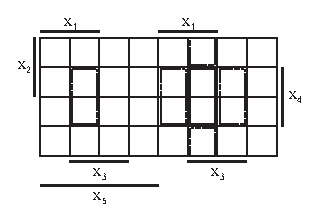
\includegraphics{veitch_sosednost-zgled-5.eps}
\end{center}
\caption{Izrazi, ki so sosedni izrazu $m_{22} \vee m_{30}$.}
\label{fig:Veitch_sosednost_zgled_5}
\end{figure}

\end{resitev}


\subsection{Določanje minimalne normalne oblike z Veitchevim diagramom}

Za minimalno normalno obliko (MNO) velja, da predstavlja krajšo izmed minimalne disjunktivne normalne oblike (MDNO) in minimalne konjunktivne normalne oblike (MKNO). Za določitev MNO moramo torej najprej določiti MDNO in MKNO.

\subsubsection{Določanje minimalne disjunktivne normalne oblike z Veitchevim diagramom}
Postopek določanja je sledeč:
\begin{enumerate}
\item Funkcijo predstavimo z Veitchevim diagramom.
\item Poiščemo glavne vsebovalnike, tako da med seboj združujemo čim večje število sosednih mintermov, pri katerih je funkcijska vrednost enaka 1. Združujemo lahko 1,2,4,8,16,... mintermov. Iščemo najmanjši nabor pokritij, s katerim pokrijemo vse enice. V vsakem koraku poskušamo dobiti čim večje pokritje, saj s tem izločimo večje število vhodnih spremenljivk.
\item Zapišemo MDNO na podlagi glavnih vsebovalnikov.
\end{enumerate}

\subsubsection{Določanje minimalne konjunktivne normalne oblike z Veitchevim diagramom}
\begin{enumerate}
\item Negirano funkcijo predstavimo z Veitchevim diagramom.
\item Poiščemo MDNO negirane funkcije.
\item Negiramo MDNO negirane funkcije, s čimer dobimo izhodiščno funkcijo.
\item Z upoštevanjem DeMorganovega pravila funkcijo prevedemo v MKNO.
\end{enumerate}

\subsubsection{Določanje minimalne normalne oblike}
\begin{enumerate}
\item Določimo število operatorjev (logičnih vrat) in operandov (vhodov) za MDNO in za MKNO posebej. Negacij ne štejemo.
\item Minimalna oblika je tista, ki ima manjše število operatorjev. Če je število operatorjev pri obeh enako, je minimalna tista, ki ima manjše število operandov.
\end{enumerate}

\begin{zgled}
Za funkcijo $f(x_1,x_2,x_3,x_4) = \vee^4(0,4,8,9,10,11,12)$ določi minimalno normalno obliko.\\
\end{zgled}
\begin{resitev}
Najprej določimo MDNO:

\begin{enumerate}
\item Narišemo Veitchev diagram funkcije in označimo glavne vsebovalnike (Slika \ref{fig:Veitch_MDNO}).

\begin{figure}[ht]
\begin{center}
	
\includegraphics{veitch_MDNO.eps}
\end{center}
\caption{Glavni vsebovalniki funkcije $\vee^4(0,4,8,9,10,11,12)$.}
\label{fig:Veitch_MDNO}
\end{figure}

\item Izpišemo glavne vsebovalnike in s tem MDNO:
$$f(x_1,x_2,x_3,x_4)=x_1 \ol x_2 \vee \ol x_3 \ol x_4$$
\end{enumerate}

Potem določimo MKNO:
\begin{enumerate}
\item Narišemo Veitchev diagram negirane funkcije $\ol{f(x_1,x_2,x_3,x_4)}$= \\$\vee^4(1,2,3,5,6,7,13,14,15)$ in označimo glavne vsebovalnike (Slika \ref{fig:Veitch_MKNO}). 
\begin{figure}[ht]
\begin{center}
	\begin{tabular}{cccc}
		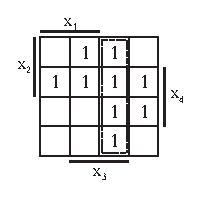
\includegraphics{veitch_MKNO1.eps} & 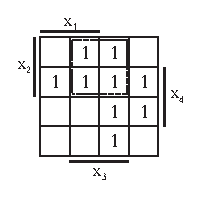
\includegraphics{veitch_MKNO2.eps} & 
\includegraphics{veitch_MKNO3.eps} & 
\includegraphics{veitch_MKNO4.eps}\\
		(a) & (b) & (c) & (d)\\
	\end{tabular}		 	
\end{center}
\caption{Glavni vsebovalniki funkcije $\vee^4(1,2,3,5,6,7,13,14,15)$. Slika (a) prikazuje glavni vsebovalnik $\ol x_1 x_3$, slika (b) $x_2 x_3$, slika (c) $\ol x_1 x_4$, slika (d) pa $x_2 x_4$.}
\label{fig:Veitch_MKNO}
\end{figure}

\item Izpišemo glavne vsebovalnike, ki določajo negirano funkcijo: $\ol{f(x_1,x_2,x_3,x_4)} = \ol x_1 x_3 \vee x_2 x_3 \vee \ol x_1 x_4 \vee x_2 x_4$. S tem dobimo MDNO negirane funkcije.
\item Dobljeno MDNO negiramo, uporabimo DeMorganovo pravilo in dobimo MKNO:  $f(x_1,x_2,x_3,x_4) = \ol{\ol x_1 x_3 \vee x_2 x_3 \vee \ol x_1 x_4 \vee x_2 x_4} = (x_1 \vee \ol x_3)(\ol x_2 \vee \ol x_3)(x_1 \vee \ol x_4)(\ol x_2 \vee \ol x_4)$.
\end{enumerate}

Sedaj lahko določimo MNO:
\begin{enumerate}
\item Določimo število operatorjev pri MDNO (za realizacijo potrebujemo dvoja AND vrata in ena OR vrata): $2+1=3$.
\item Določimo število operandov pri MDNO (2 vhoda v prva AND vrata, 2 vhoda v druga AND vrata, 2 vhoda v OR vrata): $2+2+2=6$.
\item Zapišemo par število operatorjev/število operandov za MDNO: $[3,6]$.
\item Določimo število operatorjev pri MKNO (za realizacijo potrebujemo ena AND vrata in štiri OR vrata): $1+4=5$.
\item Določimo število operandov pri MKNO (AND vrata so 4-vhodna, vsa OR vrata pa 2-vhodna): $4+4 \cdot 2=12$.
\item Zapišemo par število operatorjev/število operandov za MKNO: $[5,12]$.
\item Para leksikografsko primerjam med seboj. Ker ima MDNO manjše število operatorjev predstavlja MNO funkcije. MNO je torej $f(x_1,x_2,x_3,x_4)=x_1 \ol x_2 \vee \ol x_3 \ol x_4$.
\end{enumerate}
\end{resitev}

\begin{zgled}
Minimiziraj nepopolno preklopno funkcijo $f^4 = \vee^4(5,7,9,13) \vee^4_? (8,11,12,15)$.\\

\textbf{Opomba}: preklopna funkcija je nepopolna, če funkcijskih vrednosti nima določenih pri vseh vhodnih vektorjih.\\
\end{zgled}
\begin{resitev}

Določimo MDNO:

\begin{enumerate}
\item Narišemo Veitchev diagram funkcije in označimo glavne vsebovalnike (slika \ref{fig:Veitch_nepopolna_MDNO}) Pri tem vprašaje pokrijemo po potrebi.
\begin{figure}[ht]
\begin{center}
	
\includegraphics{veitch_nepopolna_MDNO.eps}
\end{center}
\caption{Glavni vsebovalniki funkcije $f^4 = \vee^4(5,7,9,13) \vee^4_? (8,11,12,15)$.}
\label{fig:Veitch_nepopolna_MDNO}
\end{figure}
\item Izpišemo MDNO: $f^4=x_1 x_4 \vee x_2 x_4$.
\item  Določimo število operatorjev in operandov: $[3,6]$.
\end{enumerate}

Določimo MKNO:
\begin{enumerate}
\item Narišemo Veitchev diagram negirane funkcije (kjer so bila prej prazna polja pišemo enice, kjer so bile prej enice pustimo prazno, kjer so bili prej vprašaji, pustimo vprašaje - slika \ref{fig:Veitch_nepopolna_MKNO}). Označimo glavne vsebovalnike.
\begin{figure}[ht]
\begin{center}
	
\includegraphics{veitch_nepopolna_MKNO.eps}
\end{center}
\caption{Glavni vsebovalniki funkcije $f^4 = \vee^4(0,1,2,3,4,6,10,14) \vee^4_? (8,11,12,15)$.}
\label{fig:Veitch_nepopolna_MKNO}
\end{figure}
\item Izpišemo MDNO negirane funkcije: $\ol{f^4}=\ol x_4 \vee \ol x_1 \ol x_2$.
\item Določimo MKNO: $f^4=\ol{\ol x_4 \vee \ol x_1 \ol x_2}=x_4(x_1 \vee x_2)$.
\item Določimo število operatorjev in operandov: $[2,4]$.
\end{enumerate}

Določimo MNO:
\begin{itemize}
\item Ker ima MKNO manjše število operandov je MNO zapis:$f^4=x_4(x_1 \vee x_2)$.
\end{itemize}

\end{resitev}
\chapter{Priprava na 6. laboratorijske vaje}
\section{Simetrične preklopne funkcije}

\bigskip
Funkcija je popolnoma simetrična, če lahko zamenjamo poljubni dve vhodni spremenljivki in se funkcijska vrednost ne spremeni. Naj ima funkcija $f$ izhodno vrednost 1 pri vsakem tistem vhodnem vektorju, pri katerem ima natanko $a$ vhodnih spremenljivk vrednost 1. Število $a$ tedaj imenujemo \textit{simetrijsko število} funkcije $f$. Če za funkcijo $f$ obstaja neprazna množica simetrijskih števil, je funkcija \textit{popolnoma simetrična}.

\bigskip
\begin{zgled} Zapiši PDNO funkcije $f_{\{0,2\}}(x_1,x_2,x_3)$.
\end{zgled}
\begin{resitev} 
Pomagamo si s pravilnostno tabelo:

\begin{tabular}{ccc|c}
$x_1$ & $x_2$ & $x_3$ & $f_{\{0,2\}}(x_1,x_2,x_3)$ \\
\hline
0 & 0 & 0 & 1 \\
0 & 0 & 1 & 0 \\
0 & 1 & 0 & 0 \\
0 & 1 & 1 & 1 \\
1 & 0 & 0 & 0 \\
1 & 0 & 1 & 1 \\
1 & 1 & 0 & 1 \\
1 & 1 & 1 & 0 \\
\end{tabular}

PDNO lahko preberemo neposredno iz tabele:
$$f(x_1,x_2,x_3) = \vee^3(0,3,5,6).$$
\end{resitev}

\bigskip
\begin{zgled} 
Zapiši PDNO funkcije $f_{\{0,2\}}(x_1,\ol x_2,x_3)$.
\end{zgled}
\begin{resitev}
Pomagamo si s pravilnostno tabelo:

\begin{tabular}{ccc|ccc|c}
$x_1$ & $x_2$ & $x_3$ & $x_1$ & $\ol x_2$ & $x_3$ & $f_{\{0,2\}}(x_1,\ol x_2,x_3)$ \\
\hline
0 & 0 & 0 & 0 & 1 & 0 & 0 \\
0 & 0 & 1 & 0 & 1 & 1 & 1 \\
0 & 1 & 0 & 0 & 0 & 0 & 1 \\
0 & 1 & 1 & 0 & 0 & 1 & 0 \\
1 & 0 & 0 & 1 & 1 & 0 & 1 \\
1 & 0 & 1 & 1 & 1 & 1 & 0 \\
1 & 1 & 0 & 1 & 0 & 0 & 0 \\
1 & 1 & 1 & 1 & 0 & 1 & 1 \\
\end{tabular}

PDNO lahko preberemo neposredno iz tabele:
$$f(x_1,x_2,x_3) = \vee^3(1,2,4,7).$$
\end{resitev}


\section{Quineova metoda minimizacije}
Medtem, ko so Veitchevi diagrami zelo primerni za ročno minimizacijo funkcij z manjšim številom vhodnih spremenljivk (do vključno 5), je za večje število vhodnih spremenljivk zelo zaželena avtomatizacija iskanja minimalne oblike. Pri tem se zelo dobro obnese Quineova (tudi Quine–McCluskey) metoda, ki za minimizacijo uporablja tabelaričen postopek, ki ga je enostavno sprogramirati. Metoda temelji na iskanju potrebnih glavnih vsebovalnikov na podalgi podobnega postopka kot Veitcheva metoda, le da pri tem uporablja drugačna orodja.

\subsection{Določanje MDNO}
\begin{itemize}
\item Preklopno funkcijo zapišemo v popolni disjunktivni normalni obliki (PDNO).
\item Poiščemo vse sosednje minterme in njihove glavne vsebovalnike:
\begin{enumerate}
\item Narišemo tabelo z $n$ stolpci, pri čemer je $n$ število vhodnih spremenljivk. V prvega vpišemo vse minterme, ki določajo preklopno funkcijo.
\item Izraze v stolpcu medsebojno primerjamo in ugotavljamo sosednost. Primerjamo vsakega z vsakim.
\item Sosedna izraza prečrtamo in v naslednji stolpec vpišemo njun glavni vsebovalnik.
\item Ponavljamo koraka 2 in 3, dokler ne gremo čez vse kombinacije. Pri tem upoštevamo tudi že prečrtane izraze.
\item Če v predhodnem koraku nismo našli nobenega vsebovalnika ali pa smo prišli v zadnji stolpec zaključimo.
\end{enumerate}
\item Izpišemo samo potrebne glavne vsebovalnike:
\begin{enumerate}
\item Narišemo tabelo pokritij z vrsticami, ki predstavljajo glavne vsebovalnike (samo tiste, ki niso prečrtani) in stolpci, ki predstavljajo minterme.
\item Za vsak glavni vsebovalnik označimo minterme, ki jih pokriva.
\item Poiščemo najmanjšo množico glavnih vsebovalnikov, ki skupaj pokrijejo vse minterme.
\end{enumerate}
\end{itemize}

\begin{zgled}
\label{MDNO}
Preklopno funkcijo
$
f = \vee^4(1,4,6,7,8,9,10,11,15)
$
zapiši v MDNO s Quineovo metodo minimizacije.
\end{zgled}
\begin{resitev}

S pomočjo Quineove metode zgradimo sledečo tabelo:

\begin{tabular}{cc|cc|cc|c}
& 4 & & 3 & & 2 & 1 \\
\hline
(1) & \sout{$\ol x_1 \ol x_2 \ol x_3 x_4$} & (1,6) & $\ol x_2 \ol x_3 x_4$ & (5,8) & $x_1 \ol x_2$ \\
(2) & \sout{$\ol x_1 x_2 \ol x_3 \ol x_4$} & (2,3) & $\ol x_1 x_2 \ol x_4$ & (6,7) & \\
(3) & \sout{$\ol x_1 x_2 x_3 \ol x_4$} & (3,4) & $\ol x_1 x_2 x_3$ & & \\
(4) & \sout{$\ol x_1 x_2 x_3 x_4$} & (4,9) & $x_2 x_3 x_4$ & & \\
(5) & \sout{$x_1 \ol x_2 \ol x_3 \ol x_4$} & (5,6) & \sout{$x_1 \ol x_2 \ol x_3$} & & \\
(6) & \sout{$x_1 \ol x_2 \ol x_3 x_4$} & (5,7) & \sout{$x_1 \ol x_2 \ol x_4$} & & \\
(7) & \sout{$x_1 \ol x_2 x_3 \ol x_4$} & (6,8) & \sout{$x_1 \ol x_2 x_4$} & & \\
(8) & \sout{$x_1 \ol x_2 x_3 x_4$} & (7,8) & \sout{$x_1 \ol x_2 x_3$} & & \\
(9) & \sout{$x_1 x_2 x_3 x_4$} & (8,9) & $x_1 x_3 x_4$ & & &
\end{tabular}

\bigskip
Zgradimo tabelo pokritij:


\begin{tabular}{cc|ccccccccc}
& & $m_1$ & $m_4$ & $m_6$ & $m_7$ & $m_8$ & $m_9$ & $m_{10}$ & $m_{11}$ & $m_{15}$ \\
\hline
$\checkmark$ & $\ol x_2 \ol x_3 x_4$ & $\checkmark$ & & & & & $\checkmark$ & & & \\
\hline
$\checkmark$ & $\ol x_1 x_2 \ol x_4$ & & $\checkmark$ & $\checkmark$ & & & & & & \\
\hline
& $\ol x_1 x_2 x_3$ & & & $\checkmark$ & $\checkmark$ & & & & & \\
\hline
$\checkmark$ & $x_2 x_3 x_4$ & & & & $\checkmark$ & & & & & $\checkmark$ \\
\hline
& $x_1 x_3 x_4$ & & & & & & & & $\checkmark$ & $\checkmark$ \\
\hline
$\checkmark$ & $x_1 \ol x_2$ & & & & & $\checkmark$ & $\checkmark$ & $\checkmark$ & $\checkmark$ & \\
\hline
\end{tabular}

\bigskip
Iz tabele določimo potrebne glavne vsebovalnike:
\bigskip
$f_{\text{MDNO}}(x_1,x_2,x_3,x_4) = x_1 \ol x_2 \vee x_2 x_3 x_4 \vee \ol x_1 x_2 \ol x_4 \vee \ol x_2 \ol x_3  x_4.$
\end{resitev}

\subsection{Določanje MKNO}
Postopek je podoben kot pri Veitchevi minimizaciji:
\begin{enumerate}
\item funkcijo negiramo,
\item s Quineovo metodo izračunamo MDNO negirane funkcije,
\item rezultat negiramo in z DeMorganovim pravilom pretvorimo v MKNO.
\end{enumerate}

\begin{zgled}
Preklopno funkcijo
$
f = \vee^4(1,4,6,7,8,9,10,11,15)
$
zapiši v MKNO s Quineovo metodo minimizacije.
\end{zgled}

\begin{resitev}
Funkcijo najprej negiramo:
$\ol f = \vee^4(0,2,3,5,12,13,14)$.

\bigskip
S Quineovo metodo zgradimo sledečo tabelo:

\begin{tabular}{c|c|cc}
& 4 & & 3 \\
\hline
(1) & \sout{$\ol x_1 \ol x_2 \ol x_3 \ol x_4$} & (1,2) & $\ol x_1 \ol x_2 \ol x_4$ \\
(2) & \sout{$\ol x_1 \ol x_2 x_3 \ol x_4$} & (2,3) & $\ol x_1 \ol x_2 x_3$ \\
(3) & \sout{$\ol x_1 \ol x_2 x_3 x_4$} & (4,6) & $x_2 \ol x_3 x_4$ \\
(4) & \sout{$\ol x_1 x_2 \ol x_3 x_4$} & (5,6) & $x_1 x_2 \ol x_3$ \\
(5) & \sout{$x_1 x_2 \ol x_3 \ol x_4$} & (5,7) & $x_1 x_2 \ol x_4$ \\
(6) & \sout{$x_1 x_2 \ol x_3 x_4$} && \\
(7) & \sout{$x_1 x_2 x_3 \ol x_4$} && \\
\end{tabular}

\bigskip
Zgradimo tabelo pokritij:

\begin{tabular}{cc|ccccccc}
& & $m_0$ & $m_2$ & $m_3$ & $m_5$ & $m_{12}$ & $m_{13}$ & $m_{14}$ \\
\hline
$\checkmark$ & $\ol x_1 \ol x_2 \ol x_4$ & $\checkmark$ & $\checkmark$ & & & & &  \\
\hline
$\checkmark$ & $\ol x_1 \ol x_2 x_3$ & & $\checkmark$ & $\checkmark$ & & & &  \\
\hline
$\checkmark$ & $x_2 \ol x_3 x_4$ & & & & $\checkmark$ & & $\checkmark$ &  \\
\hline
& $x_1 x_2 \ol x_3$ & & & & & $\checkmark$ & $\checkmark$ & \\
\hline
$\checkmark$ & $x_1 x_2 \ol x_4$ & & & & & $\checkmark$ & & $\checkmark$ \\
\hline
\end{tabular}

\bigskip
Iz tabele določimo potrebne glavne vsebovalnike:

$\ol f_{\text{MDNO}}(x_1,x_2,x_3,x_4) = \ol x_1 \ol x_2 \ol x_4 \vee \ol x_1 \ol x_2 x_3 \vee x_2 \ol x_3 x_4 \vee x_1 x_2 \ol x_4$

\bigskip
Funkcijo ponovno negiramo in jo preko DeMorganovega pravila pretvorimo v konjunktivno normalno obliko:
\begin{align*}
\ol{\ol f}_{\text{MDNO}}(x_1,x_2,x_3,x_4) &= f_{\text{MKNO}}(x_1,x_2,x_3,x_4) = \ol{\ol x_1 \ol x_2 \ol x_4 \vee \ol x_1 \ol x_2 x_3 \vee x_2 \ol x_3 x_4 \vee x_1 x_2 \ol x_4}  \\ &= (x_1 \vee x_2 \vee x_4)(x_1 \vee x_2 \vee \ol x_3)(\ol x_2 \vee x_3 \vee \ol x_4)(\ol x_1 \vee \ol x_2 \vee x_4)
\end{align*}


\end{resitev}

%\section*{Laboratorijske vaje}
%Z uporabo Quineove metode minimizacije zapišite funkcijo $f$ v MDNO in jo realizirajte (Logisim) s poljubnimi znanimi elementi.
%\begin{enumerate}
%\item[a)] $f_{\{0,1\}}(x_1,\ol x_2,x_3)$
%
%\begin{tabular}{ccc|c}
%$x_1$ & $x_2$ & $x_3$ & $f_{\{0,1\}}(x_1,\ol x_2,x_3)$\\
%\hline
%0 & 0 & 0 & 1 \\
%0 & 0 & 1 & 0 \\
%0 & 1 & 0 & 1 \\
%0 & 1 & 1 & 1 \\
%1 & 0 & 0 & 0 \\
%1 & 0 & 1 & 0 \\
%1 & 1 & 0 & 1 \\
%1 & 1 & 1 & 0 \\
%\end{tabular}
%
%\begin{tabular}{ccc|ccc|c}
%& 3 & & & 2 & & 1 \\
%\hline
%(1) & $\ol x_1 \ol x_2 \ol x_3$ & x & (1,2) & $\ol x_1 \ol x_3$ & &\\
%(2) & $\ol x_1 x_2 \ol x_3$ & x & (2,3) & $\ol x_1 x_2$ & &\\
%(3) & $\ol x_1 x_2 x_3$ & x & (2,4) & $x_2 \ol x_3$ & &\\
%(4) & $x_1 x_2 \ol x_3$ & x & & & &
%\end{tabular}
%
%\bigskip
%\begin{tabular}{cc|cccc}
%& & $m_0$ & $m_2$ & $m_3$ & $m_6$\\
%\hline
%$\checkmark$ & $\ol x_1 \ol x_3$ & $\checkmark$ & $\checkmark$ & & \\
%\hline
%$\checkmark$ & $\ol x_1 x_2$ & & $\checkmark$ & $\checkmark$ & \\
%\hline
%$\checkmark$ & $x_2 \ol x_3$ & & $\checkmark$ & & $\checkmark$ \\
%\hline
%\end{tabular}
%
%\bigskip
%$f_{\text{MDNO}} = \ol x_1 \ol x_3 \vee \ol x_1 x_2 \vee x_2 \ol x_3$
%
%\item[b)] $f_{\{0,1\}}(\ol x_1,x_2,\ol x_3)$
%
%\begin{tabular}{ccc|c}
%$x_1$ & $x_2$ & $x_3$ & $f_{\{0,1\}}(\ol x_1,x_2,\ol x_3)$\\
%\hline
%0 & 0 & 0 & 0 \\
%0 & 0 & 1 & 1 \\
%0 & 1 & 0 & 0 \\
%0 & 1 & 1 & 0 \\
%1 & 0 & 0 & 1 \\
%1 & 0 & 1 & 1 \\
%1 & 1 & 0 & 0 \\
%1 & 1 & 1 & 1 \\
%\end{tabular}
%
%\begin{tabular}{ccc|ccc|c}
%& 3 & & & 2 & & 1 \\
%\hline
%(1) & $\ol x_1 \ol x_2 x_3$ & x & (1,3) & $\ol x_2 x_3$ & &\\
%(2) & $x_1 \ol x_2 \ol x_3$ & x & (2,3) & $x_1 \ol x_2$ & &\\
%(3) & $x_1 \ol x_2 x_3$ & x & (3,4) & $x_1 x_3$ & &\\
%(4) & $x_1 x_2 x_3$ & x & & & &
%\end{tabular}
%
%\bigskip
%\begin{tabular}{cc|cccc}
%& & $m_1$ & $m_4$ & $m_5$ & $m_7$\\
%\hline
%$\checkmark$ & $\ol x_2 x_3$ & $\checkmark$ & & $\checkmark$ &\\
%\hline
%$\checkmark$ & $x_1 \ol x_2$ & & $\checkmark$ & $\checkmark$ &\\
%\hline
%$\checkmark$ & $x_1 x_3$ & & & $\checkmark$ & $\checkmark$\\
%\hline
%\end{tabular}
%
%\bigskip
%$f_{\text{MDNO}} = \ol x_2 x_3 \vee x_1 \ol x_2 \vee x_1 x_3$
%
%\end{enumerate}
\chapter{Priprava na 7. laboratorijske vaje}
\section{Ločenje preklopnih funkcij}

Ločenje preklopne funkcije po spremenljivki $x_i$ je definirano z izrazom

\begin{align*}
&f(x_1, x_2,..., x_{i-1}, x_i, x_{i+1},..., x_n) = \\ &f(x_1, x_2,..., x_{i-1}, 0, x_{i+1},..., x_n) \ol x_i \vee f(x_1, x_2,..., x_{i-1}, 1, x_{i+1},..., x_n) x_i 
\end{align*}

za ločenje konjunktivnih izrazov in z izrazom

\begin{align*}
&f(x_1, x_2,..., x_{i-1}, x_i, x_{i+1},..., x_n) = \\ &(f(x_1, x_2,..., x_{i-1}, 0, x_{i+1},..., x_n) \vee x_i) (f(x_1, x_2,..., x_{i-1}, 1, x_{i+1},..., x_n) \vee \ol x_i) 
\end{align*}

za ločenje disjunktivnih izrazov. Pri tem funkcijama, ki nastopata v izrazu, pravimo \emph{funkcijska ostanka}:

$$
f_0(x_1, x_2,..., x_{i-1}, x_{i+1},..., x_n) = f(x_1, x_2,..., x_{i-1}, 0, x_{i+1},..., x_n),
$$

$$
f_1(x_1, x_2,..., x_{i-1}, x_{i+1},..., x_n) = f(x_1, x_2,..., x_{i-1}, 1, x_{i+1},..., x_n).
$$

Za realizacijo preklopnih funkcij z multiplekserji uporabljamo konjunktivno ločevanje izrazov, zato bomo
v nadaljevanju obravnavali le tega.

\begin{zgled}
\label{zgled:ostanki}
Funkcijo $f(x_1, x_2, x_3) = \vee^3(0, 2, 5, 6, 7)$ loči preko spremenljivke $x_1$.
\end{zgled}
\begin{resitev}

Funkcijo lahko zapišemo kot:

\begin{align*}
	f(x_1, x_2, x_3)& = &\ol x_1 \ol x_2 \ol x_3 \vee \ol x_1 x_2 \ol x_3 \vee x_1 \ol x_2 x_3 \vee x_1 x_2 \ol x_3 \vee x_1 x_2 x_3\\
	 & = &(\ol 0 \ol x_2 \ol x_3 \vee \ol 0 x_2 \ol x_3 \vee 0 \ol x_2 x_3 \vee 0 x_2 \ol x_3 \vee 0 x_2 x_3) \ol x_1 \vee\\
	&    &\vee (\ol 1 \ol x_2 \ol x_3 \vee \ol 1 x_2 \ol x_3 \vee 1 \ol x_2 x_3 \vee 1 x_2 \ol x_3 \vee 1 x_2 x_3) x_1 \\
	& = &(\ol x_2 \ol x_3 \vee x_2 \ol x_3)\ol x_1 \vee (\ol x_2 x_3 \vee x_2 \ol x_3 \vee x_2 x_3) x_1
\end{align*}

\bigskip

Pri tem dobimo funkcijska ostanka:
\begin{align*}
&f_0(x_2,x_3)=\ol x_2 \ol x_3 \vee x_2 \ol x_3\\
&f_1(x_2,x_3)=\ol x_2 x_3 \vee x_2 \ol x_3 \vee x_2 x_3
\end{align*}

\bigskip

Ločimo funkcijski ostanek $f_0(x_2, x_3)$ še po $x_2$:
\begin{align*}
f_0(x_2,x_3)&=(\ol 0 \ol x_3 \vee 0 \ol x_3)\ol x_2 \vee (\ol 1 \ol x_3 \vee 1 \ol x_3) x_2\\
&=\ol x_3\ol x_2 \vee \ol x_3 x_2
\end{align*}

\bigskip

Pri tem dobimo funkcijska ostanka:
\begin{align*}
&f_{00}(x_3)=\ol x_3\\
&f_{01}(x_3)=\ol x_3
\end{align*}

\bigskip

Ločimo funkcijski ostanek $f_1(x_2, x_3)$ še po $x_2$:
\begin{align*}
f_1(x_2,x_3)&=(\ol 0 x_3 \vee 0 \ol x_3 \vee 0 x_3)\ol x_2 \vee (\ol 1 x_3 \vee 1 \ol x_3 \vee 1 x_3) x_2\\
&=x_3\ol x_2 \vee (\ol x_3 \vee x_3) x_2\\
&=x_3\ol x_2 \vee 1x_2
\end{align*}

\bigskip

Pri tem dobimo funkcijska ostanka:
\begin{align*}
&f_{10}(x_3)=x_3\\
&f_{11}(x_3)=1
\end{align*}

\end{resitev}

\section{Multiplekser}
Multiplekser spada v družino strukturalnih preklopnih vezij. Multiplekser ima dva niza vhodnih spremenljivk, in sicer \emph{naslovne spremenljivke} na naslovnih vhodih ($A_n,A_{n-1},...,A_0$) in \emph{podatkovne spremenljivke} na podatkovnih vhodih ($I_0, I_1,..., I_{2^n-1}$). Na podlagi vrednosti naslovnih spremenljivk se izbere podatkovni vhod, ki se bo preslikal na izhod multiplekserja. Multiplekser v kombinaciji s konstanto 0 ali 1 predstavlja funkcijsko poln sistem - z njim oziroma s kombinacijo več multiplekserjev lahko realiziramo poljubno logično funkcijo.\\

Multiplekser v odvisnosti od vrednosti naslovnih vhodov na izhod preslika enega izmed podatkovnih vhodov. Natančneje, na izhod se preslika podatkovni vhod z indeksom, ki je enak desetiškemu zapisu vrednosti na naslovnih vhodih. Splošno delovanje multiplekserja prikazuje tabela \ref{tab:mux_2n1}.\\

\begin{table}[h]
\begin{center}
\begin{tabular}{cccc|c}
$A_{n-1}$ & $A_{n-2}$ & $...$ & $A_{0}$ &  $f$ \\
\hline
0 & 0 & ... & 0 & $I_0$  		\\
0 & 0 & ... & 1 & $I_1$  		\\
. & . & ... & . & .						\\
. & . & ... & . & .						\\
. & . & ... & . & .						\\
1 & 1 & ... & 0 & $I_{2^n-2}$ \\
1 & 1 & ... & 1 & $I_{2^n-1}$ \\
\end{tabular}
\caption{Splošno delovanje multiplekserja MUX $2^n/1$.}
\label{tab:mux_2n1}
\end{center}
\end{table}

Multiplekser z $n$ naslovnimi spremenljivkami označujemo kot MUX $2^n/1$. Realizacijo funkcije z multiplekserjem praviloma podajamo z logično shemo. Splošno logično shemo za multiplekser MUX $2^n/1$
prikazuje slika \ref{fig:mux_2n1}.

\begin{figure}[ht]
\centering
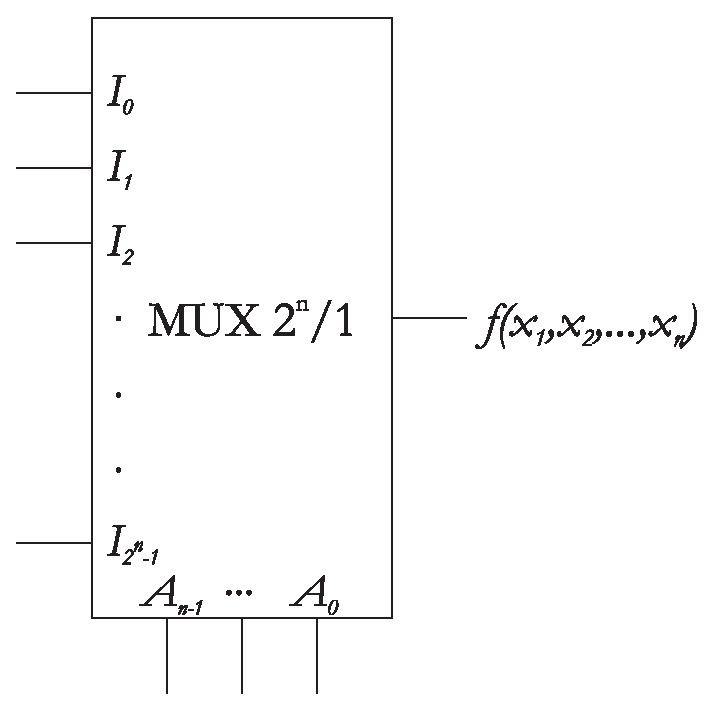
\includegraphics[width=0.5\linewidth]{mux-1.eps}
\caption{Splošna logična shema za multiplekser MUX $2^n/1$.}
\label{fig:mux_2n1}
\end{figure}

\section{Realizacija preklopnih funkcij z multiplekserji}

Z uporabo konstant 0 in 1 in multiplekserja MUX $2^n/1$ lahko realiziramo poljubno preklopno funkcijo z $n+1$ vhodnimi spremenljivkami. Realizacija funkcij z uporabo multiplekserjev z manjšim številom naslovnih vhodov poteka z drevesno oziroma kaskadno vezavo multiplekserjev.\\

Realizacija preklopnih funkcij z multiplekserji poteka na podlagi ločenja. Funkcijo ločimo preko vhodnih spremenljivk, ki jih vežemo na naslovne vhode, na podatkovnih vhodih pa realiziramo funkcijske ostanke.\\

V nadaljevanju bomo demonstrirali realizacijo funkcije $f(x_1, x_2, x_3) = \vee^3(0, 2, 5, 6, 7)$ z multiplekserji različnih velikosti.

\subsection{Število vhodnih spremenljivk je enako številu naslovnih vhodov multiplekserja}

Na razpolago imamo konstanti 0 in 1 in multiplekser, ki ima enako število naslovnih vhodov, kot je število vhodnih spremenljivk preklopne funkcije. V tem primeru na podatkovne vhode vežemo funkcijske vrednosti v enakem vrstnem redu kot ti nastopajo v pravilnostni tabeli, na naslovne vhode pa vhodne spremenljivke - prav tako v enakem vrstnem redu kot nastopajo v pravilnostni tabeli. Funkcijo torej ločimo preko vseh vhodnih spremenljivk, zato lahko vse funkcijske ostanke izrazimo s konstantami 0 in 1.

\begin{zgled}
Realiziraj funkcijo $\vee^3(0,2,5,6,7)$ z MUX $8/1$.
\end{zgled}
\begin{resitev}
V prvem koraku zapišemo pravilnostno tabelo funkcije.

\begin{center}
\begin{tabular}{ccc|c}
$x_1$ & $x_2$ & $x_3$ &  $f(x_1,x_2,x_3)$ \\
\hline
0 & 0 & 0 & 1 \\
0 & 0 & 1 & 0 \\
0 & 1 & 0 & 1 \\
0 & 1 & 1 & 0 \\
1 & 0 & 0 & 0 \\
1 & 0 & 1 & 1 \\
1 & 1 & 0 & 1 \\
1 & 1 & 1 & 1 \\
\end{tabular}
\end{center}

\bigskip

V drugem koraku na podatkovne vhode vežemo funkcijske vrednosti v enakem vrstnem redu kot ti nastopajo v pravilnostni tabeli, na naslovne vhode pa vhodne spremenljivke - prav tako v enakem vrstnem redu kot nastopajo v pravilnostni tabeli (glej sliko \ref{fig:mux_zgled_1}).

\bigskip
\begin{figure}[ht]
\centering
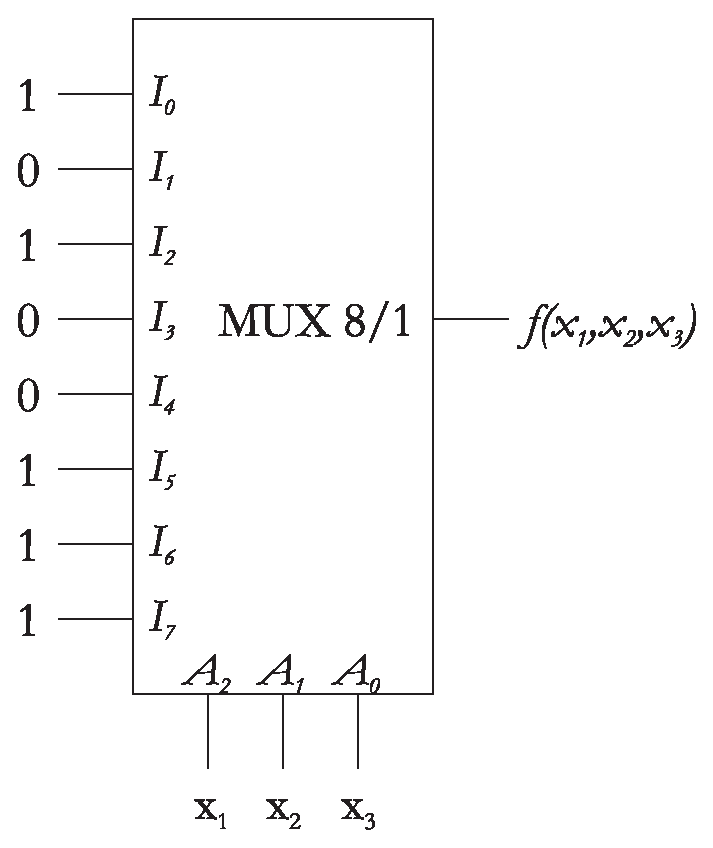
\includegraphics[width=0.5\linewidth]{mux-2.eps}
\caption{Realizacija 3-vhodne funkcije z multiplekserjem MUX $8/1$.}
\label{fig:mux_zgled_1}
\end{figure}

\end{resitev}

\subsection{Število vhodnih spremenljivk je za 1 večje od števila naslovnih vhodov multiplekserja}

Na razpolago imamo konstanti 0 in 1 in  multiplekser, ki ima število naslovnih vhodov za 1 manjše, kot je število vhodnih spremenljivk preklopne funkcije. Funkcijo ločimo po spremenljivkah glede na njihov vrstni red od leve proti desni. Iz tega sledi, da skrajno leve vhodne spremenljivke vežemo na naslovne vhode multiplekserja (najbolj levo spremenljivko na naslovni vhod z najvišjim indeksom). Na podatkovnih vhodih realiziramo funkcijski ostanek, ki ga lahko vedno izrazimo z najmanj pomembno vhodno spremenljivko, njeno negacijo, konstanto 0 in konstanto 1.

\begin{zgled}
Realiziraj funkcijo $\vee^3(0,2,5,6,7)$ z MUX $4/1$.\\
\end{zgled}
\begin{resitev}

V prvem koraku zapišemo pravilnostno tabelo funkcije.

\bigskip
\begin{center}
\begin{tabular}{ccc|cc}
$x_1$ & $x_2$ & $x_3$ &  $f(x_1,x_2,x_3)$ \\
\hline
0 & 0 & 0 & 1 &\multirow{2}{*}{$I_0=\ol x_3$}\\
0 & 0 & 1 & 0 &\\ 
\hline
0 & 1 & 0 & 1 &\multirow{2}{*}{$I_1=\ol x_3$}\\
0 & 1 & 1 & 0 &\\
\hline
1 & 0 & 0 & 0 &\multirow{2}{*}{$I_2=x_3$}\\
1 & 0 & 1 & 1 &\\
\hline
1 & 1 & 0 & 1 &\multirow{2}{*}{$I_3=1$}\\
1 & 1 & 1 & 1 &\\
\end{tabular}
\end{center}

\bigskip

V drugem koraku na naslovne vhode vežemo najpomembnejše spremenljivke (v našem primeru $x_1$ in $x_2$). V našem primeru na vhod $A_1$ vežemo $x_1$, na vhod $A_2$ pa $x_2$. S tem funkcijo ločimo preko spremenljivk $x_1$ in $x_2$. S pomočjo spremenljivke, ki je ostala, uporabe negacij, konstante 0 in 1, realiziramo funkcijske ostanke ločenja, ki jih vežemo na podatkovne vhode (glej sliko \ref{fig:mux_zgled_2}).

\end{resitev}


\bigskip
\begin{figure}[ht]
\centering
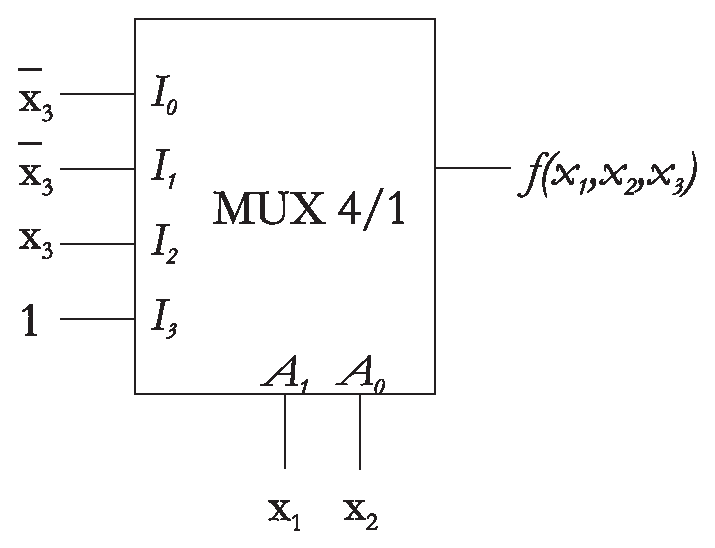
\includegraphics[width=0.5\linewidth]{mux-3.eps}
\caption{Realizacija 3-vhodne funkcije z multiplekserjem MUX $4/1$.}
\label{fig:mux_zgled_2}
\end{figure}

\subsection{Število vhodnih spremenljivk je za več kot 1 večje od števila naslovnih vhodov multiplekserja}

Če je število vhodnih spremenljivk funkcije za več kot za 1 večje od števila naslovnih vhodov multiplekserja, moramo za realizacijo uporabiti večje število multiplekserjev, ki jih med seboj vežemo v drevesno (kaskadno) vezavo. Ponavadi funkcijo ločimo po najpomembnejših spremenljivkah, ni pa to pravilo. V tem primeru začnemo z vezavo najpomembnejših spremenljivk na naslovne vhode zadnjega multiplekserja v kaskadi.

\begin{zgled}

Realiziraj funkcijo $\vee^3(0,2,5,6,7)$ z MUX $2/1$.\\

\end{zgled}
\begin{resitev}

V prvem koraku zapišemo pravilnostno tabelo in funkcijo
\begin{itemize}
\item najprej ločimo po $x_1$,
\item zgornji del (funkcijski ostanek pri $x_1=0$) lahko izrazimo z $\ol x_3$,
\item spodnji del (funkcijski ostanek pri $x_1=1$) ločimo še po $x_2$ (zgornji del, t.j. funkcijski ostanek pri $x_2 = 0$, lahko izrazimo z $x_3$, spodnji del, t.j. funkcijski ostanek pri $x_2 = 1$, pa s konstanto 1).
\end{itemize}

\bigskip

Ostanke pri ločenju smo izračunali že v zgledu \ref{zgled:ostanki}.

\begin{center}
\begin{tabular}{ccc|cc}
$x_1$ & $x_2$ & $x_3$ &  $f(x_1,x_2,x_3)$ \\
\hline
0 & 0 & 0 & 1 & \multirow{4}{*}{$\ol x_3$}\\
0 & 0 & 1 & 0 &\\ 
0 & 1 & 0 & 1 &\\
0 & 1 & 1 & 0 &\\
\hline
1 & 0 & 0 & 0 & \multirow{2}{*}{$x_3$}\\
1 & 0 & 1 & 1 &\\
\hline
1 & 1 & 0 & 1 & \multirow{2}{*}{$1$}\\
1 & 1 & 1 & 1 &\\
\end{tabular}
\end{center}

\bigskip

V drugem koraku narišemo shemo realizacije. Ker smo tabelo najprej ločili po $x_1$, $x_1$ uporabimo kot naslovni vhod zadnjega multiplekserja v kaskadi. Funkcijski ostanek $f_0$ po $x_1$ lahko izrazimo z $x_3$ -- $\ol x_3$ vežemo na podatkovni vhod $I_0$ multiplekserja. Spodnjega dela, ki predstavlja funkcijski ostanek $f_1$ po $x_1$, ne moremo izraziti na enostaven način, zato ga ločimo še po spremenljivki $x_2$ in za njegovo realizacijo uporabimo dodaten multiplekser MUX $2/1$. Le-tega vežemo na vhod $I_1$ zadnjega multiplekserja v kaskadi. Na naslovni vhod dodatnega multiplekserja vežemo spremenljivko $x_2$. Funkcijski ostanek $f_0$ ločenja po $x_2$ lahko izrazimo z $x_3$, ostanek $f_1$ pa s konstanto $1$ - razvidno iz tabele. Na podatkovni vhod $I_0$ dodatnega multiplekserja torej vežemo $x_3$, na vhod $I_1$ pa konstanto $1$. Realizacijo prikazuje slika \ref{fig:mux_zgled_3}.

\begin{figure}[ht]
\centering
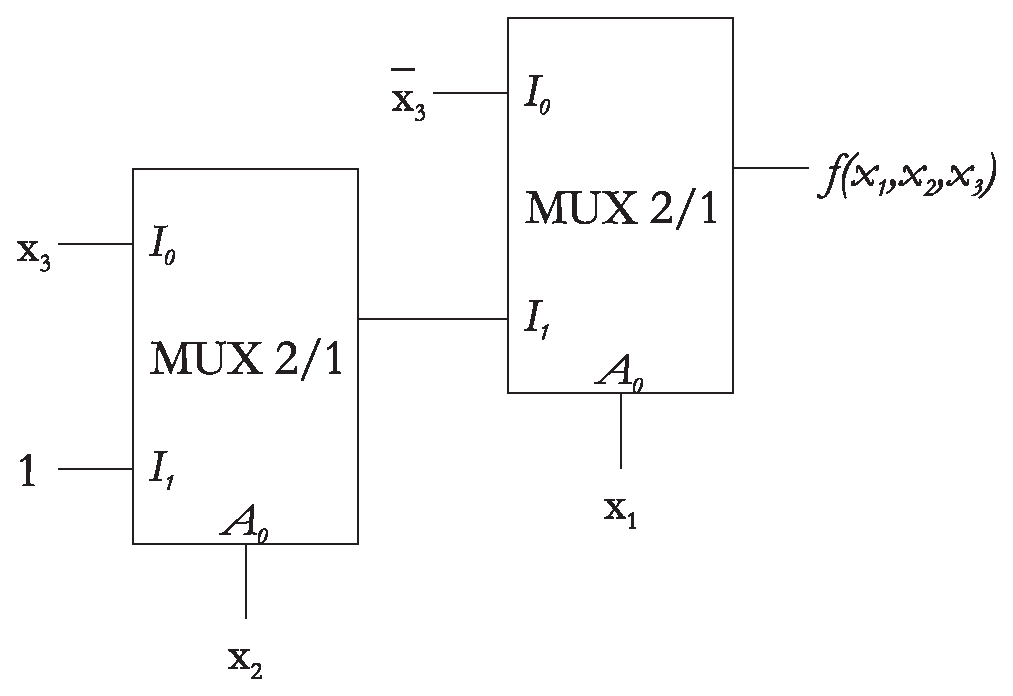
\includegraphics[width=0.75\linewidth]{mux-4.eps}
\caption{Realizacija 3-vhodne preklopne funkcije z dvema multiplekserjema MUX $2/1$.}
\label{fig:mux_zgled_3}
\end{figure}

\end{resitev}

%\section*{Laboratorijske vaje}
%Z uporabo multiplekserjev MUX 4/1 in MUX 2/1 v Logisimu realiziraj preklopno funkcijo $f(x_1,x_2,x_3,x_4) = x_1 \overline x_2 \rightarrow x_3 x_4$.
%
%\bigskip
%\begin{tabular}{cccc|c|c}
%$x_1$ & $x_2$ & $x_3$ & $x_4$ & $f$ & I\\
%\hline
%0 & 0 & 0 & 0 & 1 & \multirow{2}{*}{1}\\
%0 & 0 & 0 & 1 & 1 &\\
%\hline
%0 & 0 & 1 & 0 & 1 & \multirow{2}{*}{1}\\
%0 & 0 & 1 & 1 & 1 &\\
%\hline
%0 & 1 & 0 & 0 & 1 & \multirow{2}{*}{1}\\
%0 & 1 & 0 & 1 & 1 &\\
%\hline
%0 & 1 & 1 & 0 & 1 & \multirow{2}{*}{1}\\
%0 & 1 & 1 & 1 & 1 &\\
%\hline\hline
%1 & 0 & 0 & 0 & 0 & \multirow{2}{*}{0}\\
%1 & 0 & 0 & 1 & 0 &\\
%\hline
%1 & 0 & 1 & 0 & 0 & \multirow{2}{*}{$x_4$}\\
%1 & 0 & 1 & 1 & 1 &\\
%\hline
%1 & 1 & 0 & 0 & 1 & \multirow{2}{*}{1}\\
%1 & 1 & 0 & 1 & 1 &\\
%\hline
%1 & 1 & 1 & 0 & 1 & \multirow{2}{*}{1}\\
%1 & 1 & 1 & 1 & 1 &\\
%\end{tabular}
%
%
%
%\bigskip
%\begin{figure}[ht]
%\centering
%\includegraphics[width=0.75\linewidth]{slika_v7_1.eps}
%\end{figure}
\chapter{Priprava na 8. laboratorijske vaje}
\section{Sekvenčna vezja}
Do zdaj smo obravnavali \emph{kombinatorna vezja}, ki ne omogočajo pomnjenja. Pomnjenje je (običajno) realizirano z uporabo sinhronih pomnilnih celic (z uporabo $n$ pomnilnih celic lahko realiziramo pomnjenje $2^n$ različnih vrednosti). Izhod sinhronih pomnilnih celic se spreminja ob določeni (pozitivni ali negativni) fronti \emph{urinega signala} (angl. \emph{clock}) -- sinhronizacija z urinim signalom (glej sliko \ref{fig:urin_signal}). \emph{Sekvenčna vezja} so vezja, ki so sestavljena iz kombinatornega dela in pomnilnih celic (glej sliko \ref{fig:sekvencna}). 


\bigskip
\begin{figure}[!ht]
\centering

\includegraphics[width=0.5\linewidth]{urin.eps}
\caption{Časovni potek vzorčnega primera urinega signala. Puščica navzgor označuje pozitivno (prehod iz 0 v 1), puščica navzdol pa negativno fronto (prehod iz 1 v 0). Slika prikazuje tri periode urinega signala.}
\label{fig:urin_signal}
\end{figure}

\bigskip
\begin{figure}[!ht]
\centering
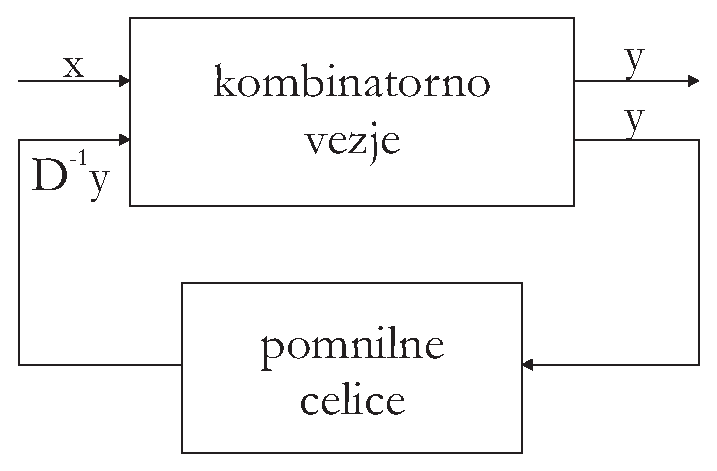
\includegraphics[width=0.3\linewidth]{sekvencna.eps}
\caption{Struktura sekvenčnih vezij.}
\label{fig:sekvencna}
\end{figure}


\section{Splošna pomnilna enačba}
Vsako sekvenčno vezje lahko zapišemo s splošno pomnilno enačbo:

$$
D^1q_i = q_i g_{i,1} \vee \ol q_i g_{i,2},
$$

pri čemer je
\begin{itemize}
\item $q_i$: ena izmed preklopnih spremenljivk, ki opisuje notranje stanje sekvenčnega vezja
\item $D^k q_i$: vrednost spremenljivke $q_i$ po $k$ časovnih korakih
\item $g_{i,1}$ in $g_{i,2}$: preklopni funkciji, odvisni od vhodnih spremenljivk $\textbf{x}=\{ x_1, x_2, ... , x_n\}$.
\end{itemize}

Novo notranje stanje sekvenčnega vezja je torej določeno s trenutnim notranjim stanjem vezja in s stanjem zunanjih vhodov. Notranje stanje se spremeni ob pozitivni ali negativni fronti urinega signala. Izbrana fronta je za celotno vezje vedno enaka, s čimer sekvenčne komponente v vezju med seboj sinhroniziramo.

\section{Enostavne pomnilne celice}
\subsection{RS pomnilna celica (\emph{Reset Set})}

RS pomnilna celica je najenostavnejša celica, katere delovanje lahko opišemo z enačbo

$$
D^1q = q \ol r \vee s,
$$
pri čemer $r$ in $s$ predstavljata zunanja vhoda v celico. Kot nakažejo že imena vhodov, vhod $r$ (\emph{reset}) izhod pomnilne celice postavi na 0, vhod $s$ ($set$) pa na 1. Če sta oba vhoda enaka 0, se izhod pomnilne celice ohranja (pomni). Za pravilno delovanje celice mora veljati pogoj $rs=0$ (vhoda ne smeta biti istočasno 1). Delovanje RS pomnilne celice lahko ponazorimo s Tabelo \ref{tab:RS}.

\begin{table}[!ht]
\begin{center}
\begin{tabular}{cc}
	\begin{tabular}{cc|c}
		$r$ & $s$ & $D^1 q$\\
		\hline
		0 & 0 & $q$\\
		0 & 1 & 1\\
		1 & 0 & 0\\
		1 & 1 & x
	\end{tabular} \hspace{1cm}
	&
	\begin{tabular}{cc|cc}
		$q$& $D^1 q$ & $r$ & $s$\\
		\hline
		0 & 0 & ? & 0\\
		0 & 1 & 0 & 1\\
		1 & 0 & 1 & 0\\
		1 & 1 & 0 & ?
	\end{tabular}
	\bigskip
	\\
	(a) & (b)
\end{tabular}
\caption{Tabela (a) prikazuje izhod RS pomnilne celice v naslednjem časovnem koraku v odvisnosti od trenutnih vhodov, (b) pa stanja vhodov, s katerimi pridemo do želenega izhoda v naslednjem časovnem koraku (vzbujevalna tabela). Pri tem x prikazuje nedefiniran izhod oziroma nedovoljeno kombinacijo vhodov.}
\label{tab:RS}
\end{center}
\end{table}

Logična simbola RS pomnilne celice sta prikazana na sliki \ref{fig:RS_shema}. 

\begin{figure}[!ht]
\begin{center}
\begin{tabular}{cc}
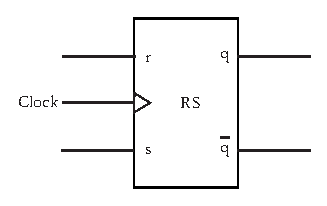
\includegraphics{RS_pos.eps} &
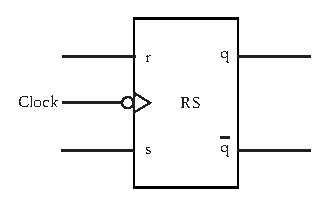
\includegraphics{RS_neg.eps} \bigskip \\
(a) & (b)
\end{tabular}
\caption{Logična simbola RS pomnilne celice, pri čemer je celica na sliki (a) sinhronizirana s pozitivno fronto urinega signala, celica na sliki (b) pa z negativno fronto.}
\label{fig:RS_shema}
\end{center}
\end{figure}


\subsection{JK pomnilna celica (\emph{Jump Kill})}
JK pomnilna celica predstavlja razširitev RS pomnilne celice. Njeno delovanje lahko opišemo z enačbo
$$
D^1q = q\ol k \vee \ol q j,
$$
kjer sta $j$ in $k$ zunanja vhoda. Če je vsaj eden izmed vhodnih signalov $j$ in $k$ enak 0, je njeno delovanje enako delovanju RS pomnilne celice. Pri tem ima signal $j$ (\emph{jump}) enako vlogo kot signal $s$, signal $k$ (\emph{kill}) pa enako vlogo kot signal $r$ RS pomnilne celice. Pri JK pomnilni celici je kombinacija vhodov $jk=1$ dovoljena. Če postavimo oba vhoda na 1, se izhod pomnilne celice ($q$) ob urini fronti zamenja ($\ol q$). Delovanje JK pomnilne celice lahko ponazorimo s Tabelo \ref{tab:JK}.

\begin{table}[!ht]
\begin{center}
\begin{tabular}{cc}
	\begin{tabular}{cc|c}
		$k$ & $j$ & $D^1 q$\\
		\hline
		0 & 0 & $q$\\
		0 & 1 & 1\\
		1 & 0 & 0\\
		1 & 1 & $\ol q$
	\end{tabular} \hspace{1cm}	&
	\begin{tabular}{cc|cc}
		$q$& $D^1 q$ & $k$ & $j$\\
		\hline
		0 & 0 & ? & 0\\
		0 & 1 & ? & 1\\
		1 & 0 & 1 & ?\\
		1 & 1 & 0 & ?
	\end{tabular}	\bigskip \\
	(a) & (b)
\end{tabular}
\caption{Tabela (a) prikazuje izhod JK pomnilne celice v naslednjem časovnem koraku v odvisnosti od trenutnih vhodov, (b) pa stanja vhodov, s katerimi pridemo do želenega izhoda v naslednjem časovnem koraku (vzbujevalna tabela).}
\label{tab:JK}
\end{center}
\end{table}

Logična simbola JK pomnilne celice sta prikazana na sliki \ref{fig:JK_shema}. 

\begin{figure}[!ht]
\begin{center}
\begin{tabular}{cc}
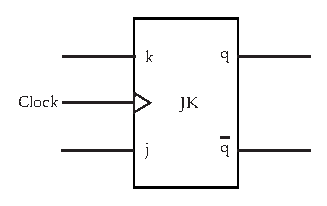
\includegraphics{JK_pos.eps} &
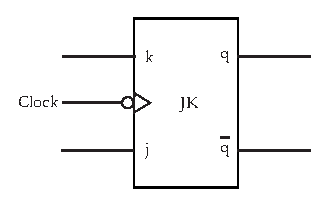
\includegraphics{JK_neg.eps} \bigskip \\
(a) & (b)
\end{tabular}
\caption{Logična simbola JK pomnilne celice, pri čemer je celica na sliki (a) sinhronizirana s pozitivno fronto urinega signala, celica na sliki (b) pa z negativno fronto.}
\label{fig:JK_shema}
\end{center}
\end{figure}

\subsection{T pomnilna celica (\emph{Trigger})}
T pomnilna celica ob fronti urinega signala spreminja izhod v primeru, da je zunanji vhod $t$ postavljen na 1, sicer pa se vrednost izhoda ohranja. Njeno delovanje lahko opišemo z enačbo
$$
D^1q = q\ol t \vee \ol q t,
$$ 
kjer je $t$ zunanji vhod. Delovanje T pomnilne celice lahko ponazorimo s Tabelo \ref{tab:T}.


\begin{table}[!ht]
\begin{center}
\begin{tabular}{cc}
	\begin{tabular}{c|c}
		$t$ & $D^1 q$\\
		\hline
		0 & $q$\\
		1 & $\ol q$
	\end{tabular} \hspace{1cm}	&
	\begin{tabular}{cc|c}
		$q$& $D^1 q$ & $t$\\
		\hline
		0 & 0 & 0\\
		0 & 1 & 1\\
		1 & 0 & 1\\
		1 & 1 & 0\\
	\end{tabular} \bigskip\\
	(a)&(b)	
\end{tabular}
\caption{Tabela (a) prikazuje notranje izhod T pomnilne celice v naslednjem časovnem koraku v odvisnosti od vrednosti vhoda, (b) pa vrednost vhoda, s katero pridemo do želenega izhoda v naslednjem časovnem koraku (vzbujevalna tabela).}
\label{tab:T}
\end{center}
\end{table}

Logična simbola T pomnilne celice sta prikazana na sliki \ref{fig:T_shema}. 

\begin{figure}[!ht]
\begin{center}
\begin{tabular}{cc}
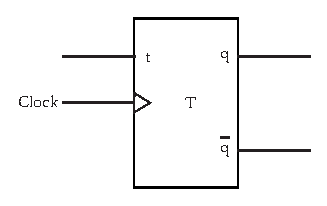
\includegraphics{T_pos.eps} &
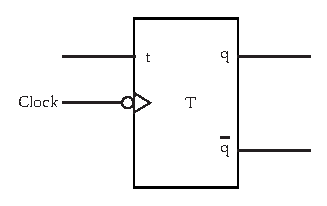
\includegraphics{T_neg.eps} \bigskip \\
(a) & (b)
\end{tabular}
\caption{Logična simbola T pomnilne celice, pri čemer je celica na sliki (a) sinhronizirana s pozitivno fronto urinega signala, celica na sliki (b) pa z negativno fronto.}
\label{fig:T_shema}
\end{center}
\end{figure}

\newpage

\subsection{D pomnilna celica (Delay)}
D pomnilna celica ob fronti urinega signala postavi svoj izhod na vrednost vhodnega signala. Njeno delovanje si lahko torej interpretiramo kot zakasnitev vhodnega signala $d$. Opišemo ga lahko z enačbo
$$
D^1q = d.
$$
Delovanje D pomnilne celice lahko ponazorimo s Tabelo \ref{tab:D}.


\begin{table}[!ht]
\begin{center}
\begin{tabular}{cc}
	\begin{tabular}{c|c}
		$d$ & $D^1 q$\\
		\hline
		0 & 0\\
		1 & 1
	\end{tabular} \hspace{1cm} &
	\begin{tabular}{cc|c}
		$q$& $D^1 q$ & $d$\\
		\hline
		0 & 0 & 0\\
		0 & 1 & 1\\
		1 & 0 & 0\\
		1 & 1 & 1\\
	\end{tabular} \bigskip\\
	(a)&(b)	
\end{tabular}
\caption{Tabela (a) prikazuje izhod D pomnilne celice v naslednjem časovnem koraku v odvisnosti od vrednosti vhoda, (b) pa vrednost vhoda, s katero pridemo do želenega izhoda v naslednjem časovnem koraku (vzbujevalna tabela).}
\label{tab:D}
\end{center}
\end{table}

Logična simbola D pomnilne celice sta prikazana na sliki \ref{fig:D_shema}. 

\begin{figure}[!ht]
\begin{center}
\begin{tabular}{cc}
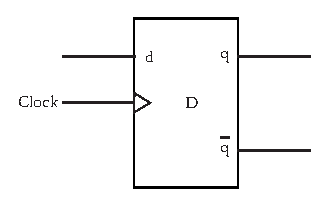
\includegraphics{D_pos.eps} &
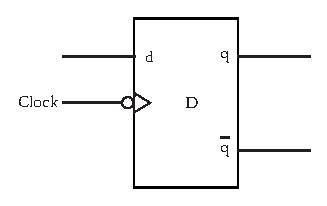
\includegraphics{D_neg.eps} \bigskip \\
(a) & (b)
\end{tabular}
\caption{Logična simbola D pomnilne celice, pri čemer je celica na sliki (a) sinhronizirana s pozitivno fronto urinega signala, celica na sliki (b) pa z negativno fronto.}
\label{fig:D_shema}
\end{center}
\end{figure}


\section{Realizacija sekvenčnih vezij s pomnilnimi celicami}

Podano imamo sekvenčno vezje in tip pomnilnih celic, ki jih lahko uporabimo za njegovo realizacijo. Naš cilj je določitev kombinatornega dela vezja, ki bo vhodne spremenljivke prilagodil delovanju danih pomnilnih celic na tak način, da bo izhod pomnilnih celic odražal delovanje podanega sekvenčnega vezja. Postopek realizacije bomo demonstirali na zgledu.

\begin{zgled}
S pomočjo JK pomnilne celice realiziraj M celico, ki deluje po enačbi $D^1 q = q(x \equiv y) \vee \ol q \; \ol y$.
\end{zgled}
\begin{resitev}
Osnutek sheme realizacije prikazuje slika \ref{fig:celica_M}. Določiti je torej potrebno kombinatorni del vezja: $k(x,y,q)$  in $j(x,y,q)$.\\

\begin{figure}[ht]
\centering
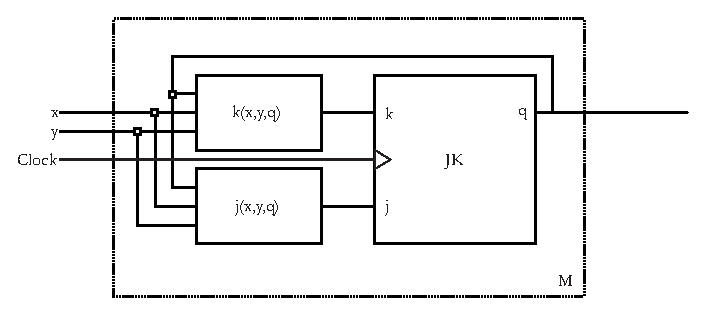
\includegraphics[width=0.75\linewidth]{sekvencna_M.eps}
\caption{Shema realizacije celice M, pri čemer $k(x,y,q)$ določa kombinatorno vezje na vhodu $k$, $j(x,y,q)$ pa kombinatorno vezje na vhodu $j$ JK pomnilne celice.}
\label{fig:celica_M}
\end{figure}

\bigskip

V prvem koraku v tabeli zapišemo funkcijo, ki določa delovanje sekvenčnega vezja. Pri tem so neodvisne spremenljivke $x$, $y$ in $q$, odvisna spremenljivka pa je $D^1 q$:

\begin{center}
\begin{tabular}{ccc|c}
$x$ & $y$ & $q$ & $D^1 q$ \\
\hline
0 & 0 & 0 & 1 \\
0 & 0 & 1 & 1 \\
0 & 1 & 0 & 0 \\
0 & 1 & 1 & 0 \\
1 & 0 & 0 & 1 \\
1 & 0 & 1 & 0 \\
1 & 1 & 0 & 0 \\
1 & 1 & 1 & 1 
\end{tabular}
\end{center}


Na podlagi prehodov iz $q$ v $D^1 q$ in na podlagi vzbujevalne tabele JK pomnilne celice (glej Tabelo \ref{tab:JK} (b)) lahko določimo vrednosti, ki morajo biti na vhodih $k$ in $j$ pri posamezni kombinaciji:

\begin{center}
\begin{tabular}{ccc|c|cc}
$x$ & $y$ & $q$ & $D^1 q$ &$k$ & $j$\\
\hline
0 & 0 & 0 & 1 & ? & 1\\
0 & 0 & 1 & 1 & 0 & ?\\
0 & 1 & 0 & 0 & ? & 0\\
0 & 1 & 1 & 0 & 1 & ?\\
1 & 0 & 0 & 1 & ? & 1\\
1 & 0 & 1 & 0 & 1 & ?\\
1 & 1 & 0 & 0 & ? & 0\\
1 & 1 & 1 & 1 & 0 & ?
\end{tabular}
\end{center}


Funkciji $k(x,y,q)$  in $j(x,y,q)$ izrazimo z vhodnimi spremenljivkami $x$, $y$ in $q$. Pri tem si lahko pomagamo z Veitchevim diagramom:

\begin{figure}[!ht]
\begin{center}
\begin{tabular}{cc}

\includegraphics{veitch_k.eps} &

\includegraphics{veitch_j.eps} \\
$k(x,y,q) = \ol x \; y \vee x \; \ol y$ & $j(x,y,q) = \ol y$\\
\end{tabular}
\end{center}
\end{figure}

\bigskip

Funkciji realiziramo v shemi, ki jo prikazuje slika \ref{fig:celica_M}.
\end{resitev}


\chapter{Priprava na 9. laboratorijske vaje}
\section{Moorov in Mealyjev končni avtomat}
Končni avtomat \angl{Finite State Machine} je določen s peterico 
$$A = \{X,S,Z,\delta,\lambda\},$$
kjer je
\begin{itemize}
\item $X$ -- vhodna abeceda: končna neprazna množica možnih vhodov v avtomat oziroma množica vhodnih črk,
\item $S$ -- notranja abeceda: končna neprazna množica možnih stanj avtomata,
\item $Z$ -- izhodna abeceda: končna neprazna množica možnih izhodov avtomata oziroma izhodnih črk,
\item $\delta$ -- funkcija prehajanja notranjih stanj: funkcija, ki v odvisnosti od trenutnega stanja in vhodne črke določa naslednje stanje avtomata,
\item $\lambda$ -- izhodna funkcija: funkcija, ki določa izhodno črko avtomata v odvisnosti od trenutnega stanja avtomata (Moorov avtomat) oziroma v odvisnosti od trenutnega stanja in vhodne črke avtomata (Mealyjev avtomat).
\end{itemize}

Avtomate navadno podajamo tabelarično s \emph{tabelo prehajanja stanj} ali grafično z \emph{diagramom prehajanja stanj}. V tabeli prehajanja stanj podajamo naslednje stanje in izhodno črko avtomata v odvisnosti od trenutnega stanja (zgornja vrstica tabele) in vhodne črke avtomata (levi stolpec tabele) kot prikazuje spodnja tabela.

\bigskip

\begin{center}
\begin{tabular}{c|c}
 & izhodna črka (Moore)\\
\hline
 & trenutno stanje\\
\hline
\multirow{6}{*}{\rottext{vhodna črka}}& \multirow{3}{*}{naslednje stanje}\\
& \\
& \\
& +\\
& \\
& izhodna črka (Mealy)\\
& 
\end{tabular}	
\end{center}

\bigskip

Diagram prehajanja stanj je podan z usmerjenim grafom, katerega vozlišča določajo stanja avtomata, povezave med vozlišči pa opisujejo prehode med stanji ob prisotnosti vhodnih črk. V primeru Moorovega avtomata stanjem pripišemo izhodno črko, ki pa je v primeru Mealyjevega avtomata vezana na prehode med stanji.

\begin{zgled}
\label{Moore_basic}
Nariši diagram prehajanja stanj za Moorov avtomat, ki je podan s sledečo tabelo prehajanja stanj

\begin{center}
\begin{tabular}{c|ccc}
 & $z_1$ & $z_1$ & $z_2$\\
 & $S_1$ & $S_2$ & $S_3$\\
\hline
$x_1$ & $S_1$ & $S_2$ & $S_1$\\
$x_2$ & $S_2$ & $S_3$ & $S_1$
\end{tabular}
\end{center}

Kakšno je zaporedje izhodnih črk (izhodna beseda), ki jo avtomat vrne pri zaporedju vhodnih črk (vhodni besedi) $x_1 x_1 x_2 x_2 x_2 x_2 x_1$ in začetnem stanju $S_1$?


\bigskip

\end{zgled}

\begin{resitev}
\hfill \break
Najprej zapišimo vse tri abecede avtomata:
\begin{itemize}
\item $X=\{x_1,x_2\}$,
\item $S=\{S_1,S_2,S_3\}$,
\item $Z=\{z_1,z_2\}$.
\end{itemize}

Diagram prehajanja stanj ima torej tri vozlišča, iz vsakega vozlišča pa vodita največ dve povezavi (za vsako vhodno črko ena):

\begin{center}
\begin{tikzpicture}[scale=0.2]
\tikzstyle{every node}+=[inner sep=0pt]
\draw [black] (16.9,-12.5) circle (3);
\draw (16.9,-12.5) node {$S_1$};
\draw (16.9,-16.7) node {$z_1$};
\draw [black] (35.9,-12.5) circle (3);
\draw (35.9,-12.5) node {$S_2$};
\draw (35.9,-16.7) node {$z_1$};
\draw [black] (26.1,-25.1) circle (3);
\draw (26.1,-25.1) node {$S_3$};
\draw (26.1,-29.2) node {$z_2$};
\draw [black] (19.9,-12.5) -- (32.9,-12.5);
\fill [black] (32.9,-12.5) -- (32.1,-12) -- (32.1,-13);
\draw (26.4,-13) node [below] {$x_2$};
\draw [black] (34.974,-15.35) arc (-22.43455:-53.31541:19.391);
\fill [black] (28.63,-23.5) -- (29.57,-23.42) -- (28.98,-22.62);
\draw (32.92,-21.27) node [right] {$x_2$};
\draw [black] (23.619,-23.419) arc (-128.64006:-159.08918:18.965);
\fill [black] (17.75,-15.38) -- (17.56,-16.3) -- (18.5,-15.94);
\draw (19.56,-21.17) node [left] {$x_1,x_2$};
\draw [black] (13.97,-13.089) arc (309.10321:21.10321:2.25);
\draw (9.61,-10.26) node [left] {$x_1$};
\fill [black] (14.65,-10.53) -- (14.53,-9.6) -- (13.76,-10.23);
\draw [black] (38.133,-10.515) arc (159.3696:-128.6304:2.25);
\draw (43.17,-10.18) node [right] {$x_1$};
\fill [black] (38.83,-13.06) -- (39.41,-13.81) -- (39.76,-12.88);
\end{tikzpicture}
\end{center}

%\begin{center}
%\begin{tikzpicture}[scale=0.2]
%\tikzstyle{every node}+=[inner sep=0pt]
%%\node[draw] at (0,0) {some text};
%\draw [black] (20.5,-17.8) circle (3);
%\draw (20.5,-17.8) node {$S_1$};
%\draw (20.5,-22) node {$z_1$};
%\draw [black] (39.7,-17.8) circle (3);
%\draw (39.7,-17.8) node {$S_2$};
%\draw (39.7,-22) node {$z_2$};
%\draw [black] (22.769,-15.848) arc (124.12588:55.87412:13.067);
%\fill [black] (37.43,-15.85) -- (37.05,-14.99) -- (36.49,-15.81);
%\draw (30.1,-13.1) node [above] {$x_2$};
%\draw [black] (37.402,-19.718) arc (-56.63019:-123.36981:13.275);
%\fill [black] (22.8,-19.72) -- (23.19,-20.58) -- (23.74,-19.74);
%\draw (30.1,-22.41) node [below] {$x_1$};
%\draw [black] (17.82,-19.123) arc (-36:-324:2.25);
%\draw (13.25,-17.8) node [left] {$x_1$};
%\fill [black] (17.82,-16.48) -- (17.47,-15.6) -- (16.88,-16.41);
%\draw [black] (42.38,-16.477) arc (144:-144:2.25);
%\draw (46.95,-17.8) node [right] {$x_2$};
%\fill [black] (42.38,-19.12) -- (42.73,-20) -- (43.32,-19.19);
%\draw [black] (42.38,-16.477) arc (144:-144:2.25);
%\fill [black] (42.38,-19.12) -- (42.73,-20) -- (43.32,-19.19);
%\end{tikzpicture}
%\end{center}

%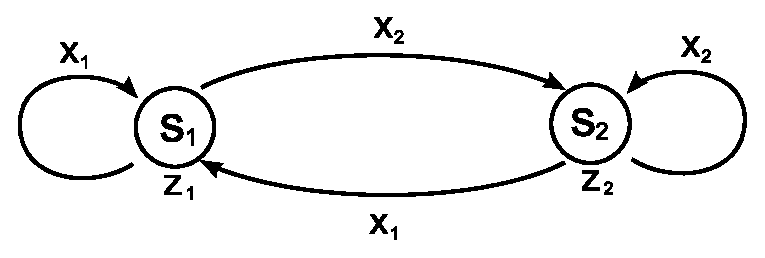
\includegraphics[width=0.5\linewidth]{slika_v9_2.eps}

\bigskip

Simulirajmo še delovanje avtomata pri vhodni besedi $x_1 x_1 x_2 x_2 x_2 x_2 x_1$ in začetnem stanju $S_1$ z uporabo spodnje tabele:

\bigskip

\begin{center}
\begin{tabular}{c|cccccccc}
vhodna črka 	&				& $x_1$ & $x_1$ & $x_2$ & $x_2$ & $x_2$ & $x_2$ & $x_1$ \\
\hline
stanje 				& $S_1$ & $S_1$ & $S_1$ & $S_2$ & $S_3$ & $S_1$ & $S_2$ & $S_2$ \\
\hline
izhodna črka	&				& $z_1$ & $z_1$ & $z_1$ & $z_2$ & $z_1$ & $z_1$ & $z_1$ 
\end{tabular}
\end{center}
\end{resitev}

\bigskip

Izhodna beseda je torej $z_1z_1z_1z_2z_1z_1z_1$.

\begin{zgled}
\label{Moore_door}
Nariši diagram prehajanja stanj in zapiši tabelo prehajanja stanj Moorovega avtomata, ki nadzira odpiranje krožnih vrat. Mehanizem drži vrata zaprta, dokler avtomat ne zazna, da je bil vstavljen kovanec. V tem primeru avtomat mehanizmu javi, da lahko sprosti zaporo vrat. Ko avtomat zazna prehod skozi vrata, ta javi mehanizmu, naj zapre vrata.
\end{zgled}

\begin{resitev}

Avtomat bo imel dve stanji, in sicer stanje, v katerem drži vrata zaprta ($S_1$) in ima tako izhodno črko $close$, in stanje, v katerem so vrata odprta ($S_2$) in ima tako izhodno črko $open$. Prehod iz $S_1$ v $S_2$ bomo izvedli, ko avtomat detektira, da je bil vstavljen kovanec (vhodna črka $coin$), prehod iz $S_2$ v $S_1$ pa, ko avtomat detektira prehod skozi vrata (vhodna črka $push$). 

\begin{center}
\begin{tikzpicture}[scale=0.2]
\tikzstyle{every node}+=[inner sep=0pt]
\draw [black] (20.5,-17.8) circle (3);
\draw (20.5,-17.8) node {$S_1$};
\draw (20.5,-22) node {$close$};
\draw [black] (39.7,-17.8) circle (3);
\draw (39.7,-17.8) node {$S_2$};
\draw (39.7,-22) node {$open$};
\draw [black] (22.769,-15.848) arc (124.12588:55.87412:13.067);
\fill [black] (37.43,-15.85) -- (37.05,-14.99) -- (36.49,-15.81);
\draw (30.1,-13.1) node [above] {$coin$};
\draw [black] (37.402,-19.718) arc (-56.63019:-123.36981:13.275);
\fill [black] (22.8,-19.72) -- (23.19,-20.58) -- (23.74,-19.74);
\draw (30.1,-22.41) node [below] {$push$};
\draw [black] (17.82,-19.123) arc (-36:-324:2.25);
\draw (13.25,-17.8) node [left] {$push$};
\fill [black] (17.82,-16.48) -- (17.47,-15.6) -- (16.88,-16.41);
\draw [black] (42.38,-16.477) arc (144:-144:2.25);
\draw (46.95,-17.8) node [right] {$coin$};
\fill [black] (42.38,-19.12) -- (42.73,-20) -- (43.32,-19.19);
\draw [black] (42.38,-16.477) arc (144:-144:2.25);
\fill [black] (42.38,-19.12) -- (42.73,-20) -- (43.32,-19.19);
\end{tikzpicture}
\end{center}

\bigskip

Zapišimo še tabelo prehajanja stanj avtomata:

\bigskip
\begin{center}
\begin{tabular}{c|cc}
&	$close$ & $open$\\
& $S_1$ & $S_2$\\
\hline
$coin$ & $S_2$ & $S_2$\\
$push$ & $S_1$ & $S_1$\\
\end{tabular}
\end{center}
\end{resitev}


\begin{zgled}
Za Mealyjev avtomat podan z diagramom prehajanja stanj zapiši tabelo prehajanja stanj. 

\bigskip

\begin{center}
\begin{tikzpicture}[scale=0.2]
\tikzstyle{every node}+=[inner sep=0pt]
\draw [black] (16.9,-12.5) circle (3);
\draw (16.9,-12.5) node {$S_1$};
\draw [black] (35.9,-12.5) circle (3);
\draw (35.9,-12.5) node {$S_2$};
\draw [black] (26.1,-25.1) circle (3);
\draw (26.1,-25.1) node {$S_3$};
\draw [black] (19.9,-12.5) -- (32.9,-12.5);
\fill [black] (32.9,-12.5) -- (32.1,-12) -- (32.1,-13);
\draw (26.4,-13) node [below] {$x_2/z_1$};
\draw [black] (34.974,-15.35) arc (-22.43455:-53.31541:19.391);
\fill [black] (28.63,-23.5) -- (29.57,-23.42) -- (28.98,-22.62);
\draw (32.92,-21.27) node [right] {$x_2/z_2$};
\draw [black] (23.619,-23.419) arc (-128.64006:-159.08918:18.965);
\fill [black] (17.75,-15.38) -- (17.56,-16.3) -- (18.5,-15.94);
\draw (19.56,-21.17) node [left] {$x_1/z_1,x_2/z_1$};
\draw [black] (13.972,-13.097) arc (309.25644:21.25644:2.25);
\draw (9.61,-10.29) node [left] {$x_1/z_1$};
\fill [black] (14.65,-10.54) -- (14.53,-9.6) -- (13.75,-10.24);
\draw [black] (38.128,-10.509) arc (159.52411:-128.47589:2.25);
\draw (43.17,-10.15) node [right] {$x_1/z_1$};
\fill [black] (38.84,-13.06) -- (39.41,-13.81) -- (39.76,-12.87);
\end{tikzpicture}
\end{center}

\bigskip

Kakšno je zaporedje izhodnih črk (izhodna beseda), ki jo avtomat vrne pri zaporedju vhodnih črk (vhodni besedi) $x_1 x_1 x_2 x_2 x_2 x_2 x_1$ in začetnem stanju $S_1$?

\end{zgled}

\begin{resitev}

Abecede avtomata so enake kot pri Moorovem avtomatu iz zgleda \ref{Moore_basic}. Zapišimo tabelo prehajanja stanj:

\begin{center}
\begin{tabular}{c|ccc}
& $S_1$ & $S_2$ & $S_3$\\
\hline
$x_1$ & $S_1/z_1$ & $S_2/z_1$ & $S_1/z_1$\\
$x_2$ & $S_2/z_1$ & $S_3/z_2$ & $S_1/z_1$
\end{tabular}
\end{center}


\bigskip

Simulirajmo še delovanje avtomata pri vhodni besedi $x_1 x_1 x_2 x_2 x_2 x_2 x_1$ in začetnem stanju $S_1$ z uporabo spodnje tabele:

\bigskip

\begin{center}
\begin{tabular}{c|cccccccc}
vhodna črka 	&				& $x_1$ & $x_1$ & $x_2$ & $x_2$ & $x_2$ & $x_2$ & $x_1$ \\
\hline
stanje 				& $S_1$ & $S_1$ & $S_1$ & $S_2$ & $S_3$ & $S_1$ & $S_2$ & $S_2$ \\
\hline
izhodna črka	&				& $z_1$ & $z_1$ & $z_1$ & $z_2$ & $z_1$ & $z_1$ & $z_1$ 
\end{tabular}
\end{center}

\bigskip

Izhodna beseda je torej $z_1z_1z_1z_2z_1z_1z_1$.

\bigskip

Avtomat pri enakih pogojih generira enako izhodno abecedo kot Moorov avtomat iz zgleda \ref{Moore_basic}. Podrobnejša analiza bi pokazala, da sta si avtomata ekvivalentna.

\bigskip

\end{resitev}


\begin{zgled}
Nariši še Mealyjev avtomat v skladu z navodili iz zgleda \ref{Moore_door}.

%Mealyjev avtomat, ki kontrolira vklop in izklop luči.\\
%$X=\{push\}$\\
%$S=\{S_{on},S_{off}\}$\\
%$Z=\{Z_{on},Z_{off}\}$\\

%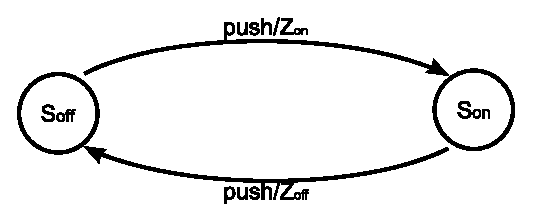
\includegraphics[width=0.5\linewidth]{slika_v9_luc_mealy.eps}

\end{zgled}

\begin{resitev}
V primeru Mealyjevega avtomata lahko avtomat z enim samim stanjem generira obe izhodni črki (\emph{open} in \emph{close}). Diagram prehajanja stanj ima tako sledečo obliko:

\begin{center}
\begin{tikzpicture}[scale=0.2]
\tikzstyle{every node}+=[inner sep=0pt]
\draw [black] (23.5,-15.1) circle (3);
\draw (23.5,-15.1) node {$S_1$};
\draw [black] (26.18,-13.777) arc (144:-144:2.25);
\draw (30.75,-15.1) node [right] {$push/close$};
\fill [black] (26.18,-16.42) -- (26.53,-17.3) -- (27.12,-16.49);
\draw [black] (20.82,-16.423) arc (-36:-324:2.25);
\draw (16.25,-15.1) node [left] {$coin/open$};
\fill [black] (20.82,-13.78) -- (20.47,-12.9) -- (19.88,-13.71);
\end{tikzpicture}
\end{center}

Zapišimo še tabelo prehajanja stanj avtomata:

\begin{center}
\begin{tabular}{c|c}
& $S_1$ \\
\hline
$coin$ & $S_1/open$ \\
$push$ & $S_1/close$
\end{tabular}
\end{center}

\end{resitev}


%%
%%
%% Pretvorbe
%%
%%

\section{Pretvorbe med avtomati}

Kot smo videli že v prejšnjih zgledih imata lahko dva avtomata različnega tipa (Moore in Mealy) popolnoma enako delovanje in sta si tako ekvivalentna (izjema je začetna izhodna črka, saj Mealyjev avtomat le-to zgenerira šele pri prvem prehodu, pri Moorovem avtomatu pa je izhodna črka vedno prisotna). V splošnem velja, da za vsak Moorov avtomat obstaja vsaj en njegov Melyjev ekvivalent in obratno. 

Pretvorbo iz Melyjevega avtomata v Moorovega lahko izvedemo po sledečem postopku:
\begin{enumerate}
\item Mealyjev avtomat zapišemo tabelarično.
\item Zapišemo vse tri abecede Moorovega avtomata, pri čemer se vhodna in izhodna abecedi ohranjata, notranjo abeceda pa tvorimo s pari notranje stanje/izhodna črka, ki se pojavijo znotraj tabele Mealyjevega avtomata.
\item Zapišemo tabelo Moorovega avtomata, v kateri nastopajo vsa stanja, ki smo jih definirali v prejšnjem koraku. Izhodna črka za stanje je določena z izhodno črko, katere oznaka nastopa pri posameznem stanju. Prehodi med stanji so določeni s prehodi med ekvivalentimi stanji v Mealyjevem avtomatu,
\end{enumerate}

\begin{zgled}
Mealyjev avtomat, podan s spodnjim diagramom, pretvori v Moorov avtomat.

\begin{center}
\begin{tikzpicture}[scale=0.2]
\tikzstyle{every node}+=[inner sep=0pt]
\draw [black] (20.5,-17.8) circle (3);
\draw (20.5,-17.8) node {$S_1$};
\draw [black] (39.7,-17.8) circle (3);
\draw (39.7,-17.8) node {$S_2$};
\draw [black] (22.769,-15.848) arc (124.12588:55.87412:13.067);
\fill [black] (37.43,-15.85) -- (37.05,-14.99) -- (36.49,-15.81);
\draw (30.1,-13.1) node [above] {$x_2/z_1$};
\draw [black] (37.402,-19.718) arc (-56.63019:-123.36981:13.275);
\fill [black] (22.8,-19.72) -- (23.19,-20.58) -- (23.74,-19.74);
\draw (30.1,-22.41) node [below] {$x_1/z_2$};
\draw [black] (17.82,-19.123) arc (-36:-324:2.25);
\draw (13.25,-17.8) node [left] {$x_1/z_1$};
\fill [black] (17.82,-16.48) -- (17.47,-15.6) -- (16.88,-16.41);
\draw [black] (42.38,-16.477) arc (144:-144:2.25);
\draw (46.95,-17.8) node [right] {$x_2/z_1$};
\fill [black] (42.38,-19.12) -- (42.73,-20) -- (43.32,-19.19);
\draw [black] (42.38,-16.477) arc (144:-144:2.25);
\fill [black] (42.38,-19.12) -- (42.73,-20) -- (43.32,-19.19);
\end{tikzpicture}
\end{center}

%\bigskip
%\includegraphics[width=0.5\linewidth]{slika_v9_3.eps}

\end{zgled}

\begin{resitev}

\bigskip
Podan Mealyjev avtomat zapišemo tabelarično:

\begin{center}
\begin{tabular}{c|cc}
 & $S_1$ & $S_2$\\
\hline
$x_1$ & $S_1/z_1$ & $S_1/z_2$\\
$x_2$ & $S_2/z_1$ & $S_2/z_1$
\end{tabular}
\end{center}

\bigskip
Notranjo abecedo Moorovega avtomata tvorijo pari naslednje stanje/izhodna črka Mealyjevega avtomata, ki se pojavijo znotraj tabele prehajanja stanj. Notranja abeceda je torej: $S_1/z_1$, $S_1/z_2$, $S_2/z_1$ (opomba: stanje $S_2/z_2$ lahko izpustimo, ker se v tabeli ne pojavi -- predpostavljamo, da to stanje ni začetno stanje avtomata). Zaradi lažjega zapisa stanja preimenujemo v: $S_{11}$, $S_{12}$, $S_{21}$. Vhodna in izhodna abeceda ostaneta enaki.

\bigskip
Na podlagi delovanja Melyjevega avtomata lahko tako zapišemo tabelo Moorovega avtomata:

\begin{center}
\begin{tabular}{c|ccc}
 & $z_1$ & $z_2$ & $z_1$\\
 & $S_{11}$ & $S_{12}$ & $S_{21}$\\
\hline
$x_1$ & $S_{11}$ & $S_{11}$ & $S_{12}$\\
$x_2$ & $S_{21}$ & $S_{21}$ & $S_{21}$
\end{tabular}
\end{center}
\bigskip
In ga narišemo.

%\includegraphics[width=0.4\linewidth]{slika_v9_4.eps}
\begin{center}
\begin{tikzpicture}[scale=0.2]
\tikzstyle{every node}+=[inner sep=0pt]
\draw [black] (19.5,-25.7) circle (3);
\draw (19.5,-25.7) node {$S_{12}$};
\draw (19.5,-29.9) node {$z_2$};
\draw [black] (39.8,-25.7) circle (3);
\draw (39.8,-25.7) node {$S_{21}$};
\draw (39.8,-29.8) node {$z_1$};
\draw [black] (29.6,-9.9) circle (3);
\draw (29.6,-9.9) node {$S_{11}$};
\draw (29.6,-14) node {$z_1$};
\draw [black] (21.827,-23.816) arc (123.00949:56.99051:14.359);
\fill [black] (37.47,-23.82) -- (37.07,-22.96) -- (36.53,-23.8);
\draw (29.65,-21) node [above] {$x_2$};
\draw [black] (37.446,-27.551) arc (-57.7201:-122.2799:14.597);
\fill [black] (21.85,-27.55) -- (22.26,-28.4) -- (22.8,-27.56);
\draw (29.65,-30.31) node [below] {$x_1$};
\draw [black] (42.48,-24.377) arc (144:-144:2.25);
\draw (47.05,-25.7) node [right] {$x_2$};
\fill [black] (42.48,-27.02) -- (42.83,-27.9) -- (43.42,-27.09);
\draw [black] (42.48,-24.377) arc (144:-144:2.25);
\fill [black] (42.48,-27.02) -- (42.83,-27.9) -- (43.42,-27.09);
\draw [black] (28.277,-7.22) arc (234:-54:2.25);
\draw (29.6,-2.65) node [above] {$x_1$};
\fill [black] (30.92,-7.22) -- (31.8,-6.87) -- (30.99,-6.28);
\draw [black] (18.272,-22.974) arc (-164.06157:-261.11516:10.332);
\fill [black] (26.61,-9.93) -- (25.74,-9.56) -- (25.9,-10.55);
\draw (18.88,-13.26) node [left] {$x_1$};
\draw [black] (32.563,-9.511) arc (88.71632:-23.0262:9.813);
\fill [black] (41.37,-23.16) -- (42.15,-22.62) -- (41.23,-22.23);
\draw (41.21,-12.68) node [right] {$x_2$};
\end{tikzpicture}
\end{center}

\bigskip
\end{resitev}

Po podobnem postopku lahko izvedemo pretvorbo Moorovega v Mealyjev avtomat:
\begin{enumerate}
\item Moorov avtomat zapišemo tabelarično.
\item Zapišemo vse tri abecede Mealyjevega avtomata, ki so kar enake abecedam Moorovega avtomata.
\item Zapišemo tabelo Mealyjevega avtomata, pri čemer je naslednje stanje enako kot pri Moorovem avtomatu, izhodna črka pa je določena z izhodno črko stanja Moorovega avtomata, v katerega bo avtomat z določeno kombinacijo stanje/vhodna črka prišel.
\end{enumerate}



\begin{zgled}

Moorov avtomat, ki predstavlja rešitev prejšnjega zgleda, pretvori v Mealyjev avtomat.

\end{zgled}

\begin{resitev}

Pretvorimo dobljeni Moorov avtomat nazaj v Mealyjevega. Vse tri abecede se ohranjajo. Zapišimo tabelo prehajanja stanj:

\begin{center}
\begin{tabular}{c|ccc}
 & $S_{11}$ & $S_{12}$ & $S_{21}$\\
\hline
$x_1$ & $S_{11}/z_1$ & $S_{11}/z_1$ & $S_{12}/z_2$\\
$x_2$ & $S_{21}/z_1$ & $S_{21}/z_1$ & $S_{21}/z_1$
\end{tabular}
\end{center}


Dobili smo avtomat s tremi notranji stanji, ki je enakovreden prvotnemu Mealyjevemu avtomatu z dvema stanjema. Stanji $S_{11}$ in $S_{12}$ sta enaki tako po izhodnih črkah kot tudi po prehodih. Stanji lahko tako zakodiramo zgolj z enim notranjim stanjem -- recimo mu stanje $S_1$. Stanje $S_{21}$ preimenujmo, da bo zapis avtomata bolj pregleden -- recimo mu stanje $S_2$. Nad stanji avtomata tako izvedemo sledečo preslikavo:
$S_{11} \rightarrow S_1$\\
$S_{12} \rightarrow S_1$\\
$S_{21} \rightarrow S_2$\\

\bigskip

Tako dobimo avtomat, ki je enak izhodiščnemu:

\begin{center}
\begin{tabular}{c|cc}
 & $S_1$ & $S_2$\\
\hline
$x_1$ & $S_1/z_1$ & $S_1/z_2$\\
$x_2$ & $S_2/z_1$ & $S_2/z_1$
\end{tabular}
\end{center}

\bigskip

\end{resitev}
\chapter{Priprava na 10. laboratorijske vaje}
\section{Realizacija končnih avtomatov s pomnilnimi celicami (Moorov avtomat)}

Z uporabo logičnih vrat in pomnilnih celic želimo realizirati Moorov avtomat. Postopek realizacije je sestavljen iz sledečih korakov:
\begin{enumerate}
\item \emph{Zapis kodirnih tabel}: vhodna abeceda, notranja abeceda in izhodna abeceda so predstavljene z abstraktnim zapisom. Za realizacijo s preklopnimi funkcijami moramo le-te predstaviti s preklopnimi spremenljivkami. Pri tem upoštevamo dejstvo, da lahko z $i$ vhodnimi spremenljivkami zakodiramo $2^i$ vhodnih črk, z $j$ izhodnimi spremenljivkami $2^j$ izhodnih črk, s $k$ pomnilnimi celicami pa $2^k$ notranjih stanj. S kodiranimi tabelami povežemo posamezne spremenljivke oziroma notranja stanja pomnilnih celic s posameznimi črkami oziroma stanji avtomata.
\item \emph{Zapis pravilnostne tabele avtomata}: na podlagi diagrama prehajanja stanj oziroma tabele prehajanja stanj in kodirnih tabel, lahko zapišemo pravilnostno tabelo avtomata. Pri tem na levi strani tabele nastopajo spremenljivke, ki določajo vhodne črke in trenutna notranja stanja avtomata (neodvisne spremenljivke), na desni strani pa spremenljivke, ki določajo notranje stanje avtomata v naslednjem časovnem koraku in spremenljivke, ki določajo izhodne črke avtomata (odvisne spremenljivke).
\item \emph{Določitev vhodov v pomnilne celice}: na podlagi prehodov med spremenljivkami, ki določajo trenutno stanje avtomata in stanje avtomata v naslednjem časovnem koraku ter vzbujevalnih tabel pomnilnih celic, ki jih imamo na razpolago, lahko določimo potrebne vhode v pomnilne celice v posamezni vrstici (tabelo dopolnimo na podoben način kot smo jo pri realizaciji sekvenčnih vezij s pomnilnimi celicami). 
\item \emph{Izpis in minimizacija izhodne funkcije in funkcije prehajanja stanj}: na podlagi pravilnostne tabele lahko s pomočjo Veitchevega diagrama izpišemo preklopne funkcije, ki določajo izhodne črke avtomata (izhodna funkcija) in preklopne funkcije, ki nastopajo na vhodih pomnilnih celic in tako določajo prehode med stanji avtomata (funkcija prehajanja stanj)
\end{enumerate}

\bigskip

\begin{zgled}

Z uporabo T pomnilnih celic in poljubnih logičnih vrat realiziraj Moorov avtomat, ki je podan z diagramom prehajanja stanj.

%\begin{center}
%\includegraphics[width=0.5\linewidth]{slika_v10_1.eps}
%\end{center}

\begin{center}
\begin{tikzpicture}[scale=0.2]
\tikzstyle{every node}+=[inner sep=0pt]
%\node[draw] at (0,0) {some text};
\draw [black] (20.5,-17.8) circle (3);
\draw (20.5,-17.8) node {$S_1$};
\draw (20.5,-22) node {$z_2$};
\draw [black] (39.7,-17.8) circle (3);
\draw (39.7,-17.8) node {$S_2$};
\draw (39.7,-22) node {$z_1$};
\draw [black] (22.769,-15.848) arc (124.12588:55.87412:13.067);
\fill [black] (37.43,-15.85) -- (37.05,-14.99) -- (36.49,-15.81);
\draw (30.1,-13.1) node [above] {$x_1$};
\draw [black] (37.402,-19.718) arc (-56.63019:-123.36981:13.275);
\fill [black] (22.8,-19.72) -- (23.19,-20.58) -- (23.74,-19.74);
\draw (30.1,-22.41) node [below] {$x_2$};
\draw [black] (17.82,-19.123) arc (-36:-324:2.25);
\draw (13.25,-17.8) node [left] {$x_2$};
\fill [black] (17.82,-16.48) -- (17.47,-15.6) -- (16.88,-16.41);
\draw [black] (42.38,-16.477) arc (144:-144:2.25);
\draw (46.95,-17.8) node [right] {$x_1$};
\fill [black] (42.38,-19.12) -- (42.73,-20) -- (43.32,-19.19);
\draw [black] (42.38,-16.477) arc (144:-144:2.25);
\fill [black] (42.38,-19.12) -- (42.73,-20) -- (43.32,-19.19);
\end{tikzpicture}
\end{center}

\end{zgled}

\begin{resitev}

Postopek je sledeč:

\begin{enumerate} 

\item Zapišemo kodirne tabele, ki določijo kodiranje vhodne abecede, notranje abecede in izhodne abecede. Za zapis vseh črk vhodne abecede je dovolj ena vhodna spremenljivka ($x$); prav tako je za zapis vseh črk izhodne abecede dovolj ena izhodna spremenljivka ($y$). Ker imamo zgolj dve notranji stanji avtomata, je za njegovo realizacijo potrebna ena pomnilna celica T z notranjim stanjem $q$. Kodirne tabele so torej

\begin{table}[ht]
\begin{center}
\begin{tabular}{ccc}
	\begin{tabular}{c|c}
	 & $x$ \\ 
		\hline
		$x_1$ & $0$\\
		$x_2$ & $1$\\
	\end{tabular}
	&
	\begin{tabular}{c|c}
		 & $q$ \\ 
		\hline
		$S_1$ & $0$\\
		$S_2$ & $1$\\
	\end{tabular}
	&
	\begin{tabular}{c|c}
		 & $y$ \\ 
		\hline
		$z_1$ & $0$\\
		$z_2$ & $1$\\
	\end{tabular}
\end{tabular}
\end{center}
\end{table}

\bigskip

\item Na podlagi kodirnih tabel in podanega diagrama prehajanja stanj lahko zapišemo pravilnostno tabelo avtomata. Pri tem na levi strani tabele nastopajo spremenljivke, ki določajo trenutno notranje stanje avtomata ($q$) in vhodno črko ($x$), na desni pa spremenljivke, ki določajo notranje stanje avtomata v naslednjem časovnem koraku ($D^1q$) in izhodno črko ($y$):

\begin{center}
\begin{tabular}{cc|cc}
 $q$ & $x$ & $D^1 q$ & $y$\\
 \hline
 0 & 0 & 1 & 1\\		 
 0 & 1 & 0 & 1\\
 1 & 0 & 1 & 0\\
 1 & 1 & 0 & 0\\
\end{tabular}
\end{center}

\bigskip

\item Na podlagi prehodov med spremenljivkami $q$ in $D^1q$ in vzbujevalne tabele za T pomnilno celico, lahko določimo vrednosti, ki morajo biti na vhodu $t$ pri posamezni kombinaciji vhodnih spremenljivk:

\begin{center}
\begin{tabular}{cc|cc|c}
 $q$ & $x$ & $D^1 q$ & $y$ & $t$\\
 \hline
 0 & 0 & 1 & 1 & 1 \\		 
 0 & 1 & 0 & 1 & 0 \\
 1 & 0 & 1 & 0 & 0 \\
 1 & 1 & 0 & 0 & 1 \\
\end{tabular}
\end{center}

\bigskip

\item Na podlagi pravilnostne tabele lahko s pomočjo Veitchevega diagrama izpišemo funkcijo, ki nastopa na vhodu T pomnilne celice in izhodno funkcijo avtomata:


\begin{figure}[!ht]
\begin{center}
\begin{tabular}{cc}
\includegraphics{veitch_moore_t.eps} &
\includegraphics{veitch_moore_y.eps} \\
$t = \ol x\ \ol q \vee x q = x \equiv q$ & $y = \ol q$\\
\end{tabular}
\end{center}
\end{figure}


Če funkcijo na vhodu T pomnilne celice vstavimo v enačbo T pomnilne celice ($D^1 q = t \ol q \vee \ol t q$), dobimo \emph{funkcijo prehajanja stanj} avtomata:
$$
D^1q = (x \equiv q) \ol q \vee \ol{(x \equiv q)} q = (x \equiv q) \ol q \vee (x \nabla q) q 
$$ 

Po definiciji velja, da je izhodna črka Moorovega avtomata določena s trenutnim stanjem avtomata. Velja torej, da je izhodno črko pri Moorovem avtomatu vedno mogoče izraziti zgolj s spremenljivkami, ki določajo trenutno stanje avtomata (v našem primeru $y=\ol q$).

\end{enumerate}

\bigskip

Realizacijo avtomata v Logisimu prikazuje slika \ref{fig:logisim1}.


\begin{figure}[ht]
\begin{center}
\includegraphics[width=0.75\linewidth]{moore_logisim_1.eps}
\end{center}
\caption{Realizacija avtomata iz zgleda v Logisimu.}
\label{fig:logisim1}
\end{figure}

\end{resitev}

\newpage

\begin{zgled}

Z uporabo D pomnilnih celic realiziraj Moorov avtomat, podan s tabelo

\begin{center}
\begin{tabular}{c|ccc}
& $z_1$ & $z_2$ & $z_3$\\
& $S_1$ & $S_2$ & $S_3$\\
\hline
$x_1$ & $S_1$ & $S_1$ & $S_1$\\
$x_2$ & $S_2$ & $S_3$ & $S_2$\\
\end{tabular}
\end{center}

\end{zgled}

\begin{resitev}
Postopek je sledeč:

\begin{enumerate} 
\item Za zapis dveh črk vhodne abecede je dovolj ena vhodna spremenljivka ($x$). Ker ima izhodna abeceda tri črke, za njen zapis potrebujemo dve spremenljivki ($y_1$ in $y_2$). Ker imamo tri notranja stanja avtomata, sta za njegovo realizacijo potrebni dve pomnilni celici D z notranjimi stanji $q_1$ in $q_2$. Kodirne tabele so torej

\begin{table}[ht]
\begin{center}
\begin{tabular}{ccc}
\begin{tabular}{c|c}
& $x$\\
\hline
$x_1$ & $0$\\
$x_2$ & $1$
\end{tabular}
&
\begin{tabular}{c|cc}
& $q_1$ & $q_2$\\
\hline
$S_1$ & $0$ & $0$\\
$S_2$ & $0$ & $1$\\
$S_3$ & $1$ & $0$
\end{tabular}
&
\begin{tabular}{c|cc}
& $y_1$ & $y_2$\\
\hline
$z_1$ & $0$ & $0$\\
$z_2$ & $0$ & $1$\\
$z_3$ & $1$ & $0$
\end{tabular}
\end{tabular}
\end{center}
\end{table}

\bigskip

\item Zapišemo pravilnostno tabelo avtomata (ko je $q_1=1$ in $q_2=1$, funkcijska vrednost ni določena):

\begin{center}
\begin{tabular}{ccc|cccc}
$q_1$ & $q_2$ & $x$ & $D^1 g_1$ & $D^1 g_2$ & $y_1$ & $y_2$\\
\hline
0 & 0 & 0 & 0 & 0 & 0 & 0\\
0 & 0 & 1 & 0 & 1 & 0 & 0\\
0 & 1 & 0 & 0 & 0 & 0 & 1\\
0 & 1 & 1 & 1 & 0 & 0 & 1\\
1 & 0 & 0 & 0 & 0 & 1 & 0\\
1 & 0 & 1 & 0 & 1 & 1 & 0\\
1 & 1 & 0 & ? & ? & ? & ?\\
1 & 1 & 1 & ? & ? & ? & ?\\
\end{tabular}
\end{center}

\bigskip

\item Na podlagi prehodov iz spremenljivke $q_1$ v $D^1q_1$ ter prehodov iz spremenljivke $q_2$ v $D^1q_2$, lahko določimo vrednosti, ki morajo biti na vhodu D pomnilnih celic (pomnilna celica z vhodom $d_1$ bo hranila notranje stanje $q_1$, celica z vhodom $d_2$ pa $q_2$):

\begin{center}
\begin{tabular}{ccc|cccc|cc}
$q_1$ & $q_2$ & $x$ & $D^1 g_1$ & $D^1 g_2$ & $y_1$ & $y_2$ & $d_1$ & $d_2$\\
\hline
0 & 0 & 0 & 0 & 0 & 0 & 0 & 0 & 0\\
0 & 0 & 1 & 0 & 1 & 0 & 0 & 0 & 1\\
0 & 1 & 0 & 0 & 0 & 0 & 1 & 0 & 0\\
0 & 1 & 1 & 1 & 0 & 0 & 1 & 1 & 0\\
1 & 0 & 0 & 0 & 0 & 1 & 0 & 0 & 0\\
1 & 0 & 1 & 0 & 1 & 1 & 0 & 0 & 1\\
1 & 1 & 0 & ? & ? & ? & ? & ? & ?\\
1 & 1 & 1 & ? & ? & ? & ? & ? & ?\\
\end{tabular}
\end{center}

\bigskip

\item Določimo funkcije za realizacijo:


\begin{figure}[!ht]
\begin{center}
\begin{tabular}{cc}
\includegraphics{veitch_moore_d_1.eps} &
\includegraphics{veitch_moore_d_2.eps} \\
$d_1 = q_2 x$ & $d_2 = \ol q_2 x$\\
\end{tabular}
\end{center}
\end{figure}

\begin{figure}[!ht]
\begin{center}
\begin{tabular}{cc}
\includegraphics{veitch_moore_y_1.eps} &
\includegraphics{veitch_moore_y_2.eps} \\
$y_1 = q_1$ & $y_2 = q_2$\\
\end{tabular}
\end{center}
\end{figure}

\bigskip



Realizacijo avtomata v Logisimu prikazujejo slike \ref{fig:logisim2}, \ref{fig:logisim2_d}(a) in \ref{fig:logisim2_d}(b).

\begin{figure}[ht]
\begin{center}
\includegraphics[width=0.75\linewidth]{moore_logisim_2.eps}
\end{center}
\caption{Realizacija avtomata iz zgleda v Logisimu. Zaradi splošnosti sheme sta funkciji, ki vstopata v pomnilni celici D, umeščeni v ločena modula (glej sliki \ref{fig:logisim2_d}(a) in \ref{fig:logisim2_d}(b)).}
\label{fig:logisim2}
\end{figure}


\begin{figure}[!ht]
\begin{center}
\begin{tabular}{cc}
\includegraphics[width=0.4\linewidth]{moore_logisim_2_d1.eps} &
\includegraphics[width=0.4\linewidth]{moore_logisim_2_d2.eps} \\
(a) & (b) \\
\end{tabular}
\caption{Realizacija preklopne funkcije, ki vstopa v D pomnilno celico z vhodom $d_1$ (a) in preklopne funkcije, ki vstopa v D pomnilno celico z vhodom $d_2$ (b).}
\label{fig:logisim2_d}
\end{center}
\end{figure}

%\bigskip
%Funkcija prehajanja stanj:\\
%$t_1(g_1, g_2, x) = g_1 \vee g_2 x$\\
%$t_2(g_1, g_2, x) = q_2 \vee x$

%\bigskip
%Izhodna funkcija:\\
%$y_1(q_1, q_2) = q_1$\\
%$y_2(q_1, q_2) = q_2$

\end{enumerate}
\end{resitev}
\chapter{Priprava na 11. laboratorijske vaje}
\section{Realizacija končnih avtomatov s pomnilnimi celicami (Mealyjev avtomat)}

Obnašanje Moorovega avtomata je že v osnovi sinhrono. Stanje avtomata se v odvisnosti od vhodne črke spremeni le ob urini fronti. Ker je izhodna črka neposredno odvisna le od njegovega stanja, se ta sinhrono spremeni ob spremembi stanja avtomata.\\

%Za razliko od Moorovega avtomata je pri Mealyjevemu avtomatu izhodna črka neposredno odvisna od stanja avtomata in vhodne črke. To pomeni, da se v primeru sprembe vhodne črke, izhodna črka lahko spremeni asinhrono (spremeni se v trenutku spremembe vhodne črke in ne le ob urini fronti oziroma spremembi stanja avtomata). Tako obnašanje ni dovoljeno in zahteva eksplicitno sinhronizacijo izhodne črke. To najenostavneje dosežemo tako, da izhodno vezje (realizacijo izhodne funkcije) vežemo na vhode D pomnilnih celic (pri realizaciji Mealyjevega avtomata z $n$ izhodnimi črkami torej potrebujemo še $\left\lceil \log_2(n)\right\rceil$ dodatnih D pomnilnih celic). S tem dosežemo, da se izhodna črka spremeni ob urini fronti, torej sinhrono s spremembo stanja avtomata.

Za razliko od Moorovega avtomata je pri Mealyjevem avtomatu izhodna črka neposredno odvisna od stanja avtomata in vhodnih spremenljivk. To pomeni, da se v primeru spremembe vhodne spremenljivke, izhodna črka lahko spremeni asinhrono (spremeni se v trenutku spremembe vhodne spremenljivke in ne le ob urini fronti oziroma spremembi stanja avtomata). Tako obnašanje ni dovoljeno in zahteva eksplicitno sinhronizacijo izhodne črke. To najenostavneje dosežemo tako, da izhodno vezje (realizacijo izhodne funkcije) vežemo na vhode D pomnilnih celic (pri realizaciji Mealyjevega avtomata z $n$ izhodnimi črkami torej potrebujemo še $\left\lceil \log_2(n)\right\rceil$ dodatnih D pomnilnih celic). S tem dosežemo, da se izhodna črka spremeni ob urini fronti, torej sinhrono s spremembo stanja avtomata.

Realizacija Mealyjevega avtomata je zelo podobna realizaciji Moorovega avtomata. Ponazorili jo bomo z zgledom, ki sledi.

\bigskip

\begin{zgled}

Realiziraj Mealyjev avtomat, ki je podan s tabelo prehajanja stanj. Za realizacijo notranjih stanj imaš na voljo T pomnilne celice, za generiranje izhodne črke pa D pomnilne celice. 

\begin{center}
\begin{tabular}{c|ccc}
 & $S_1$ & $S_2$ & $S_3$\\
\hline
$x_1$ & $S_2 / z_1$ & $S_2 / z_2$ & $S_1 / z_1$\\
$x_2$ & $S_1 / z_2$ & $S_3 / z_1$ & $S_3/ z_2$ \\
\end{tabular}
\end{center}

\end{zgled}

\begin{resitev}

Postopek je sledeč:

\begin{enumerate} 

\item Zapišemo kodirne tabele, ki določijo kodiranje vhodne abecede, notranje abecede in izhodne abecede. Za zapis vseh črk vhodne abecede je dovolj 1 vhodna spremenljivka ($x$); prav tako je za zapis vseh črk izhodne abecede dovolj 1 izhodna spremenljivka ($y$). Ker imamo tri notranja stanja avtomata, za njegovo realizacijo potrebujemo 2 pomnilni celici T z notranjimi stanji $q_1$ in $q_2$. Kodirne tabele so torej

\begin{table}[ht]
\begin{center}
\begin{tabular}{ccc}
	\begin{tabular}{c|c}
	 & $x$ \\ 
		\hline
		$x_1$ & $0$\\
		$x_2$ & $1$\\
	\end{tabular}
	&
	\begin{tabular}{c|cc}
		 & $q_1$ & $q_2$ \\ 
		\hline
		$S_1$ & $0$ & $0$ \\
		$S_2$ & $0$ & $1$\\
		$S_3$ & $1$ & $0$\\
	\end{tabular}
	&
	\begin{tabular}{c|c}
		 & $y$ \\ 
		\hline
		$z_1$ & $0$\\
		$z_2$ & $1$\\
	\end{tabular}
\end{tabular}
\end{center}
\end{table}

\bigskip

\item Na podlagi kodirnih tabel in podanega diagrama prehajanja stanj lahko zapišemo pravilnostno tabelo avtomata. Pri tem na levi strani tabele nastopajo spremenljivke, ki določajo trenutno notranje stanje avtomata ($q_1$ in $q_2$) in vhodno črko ($x$), na desni pa spremenljivke, ki določajo notranje stanje  ($D^1q_1$ in $D^1q_2$) in izhodno črko ($D^1y$) v naslednjem časovnem koraku. Vrednosti izhodne črke določamo na podlagi prehodov med stanji.

\begin{center}
\begin{tabular}{ccc|ccc}
 $q_1$ & $q_2$ & $x$ & $D^1 q_1$ & $D^1 q_2$ & $D^1y$\\
  \hline
 0 & 0 & 0 & 0 & 1 & 0\\		 
 0 & 0 & 1 & 0 & 0 & 1\\		 
 0 & 1 & 0 & 0 & 1 & 1\\		 
 0 & 1 & 1 & 1 & 0 & 0\\		 
 1 & 0 & 0 & 0 & 0 & 0\\		 
 1 & 0 & 1 & 1 & 0 & 1\\		 
 1 & 1 & 0 & ? & ? & ?\\		 
 1 & 1 & 1 & ? & ? & ?\\		 
\end{tabular}
\bigskip
\bigskip
\end{center}

\item Na podlagi prehodov med spremenljivkami $q_1$ in $D^1q_1$ ter $q_2$ in $D^1q_2$ in vzbujevalne tabele za T pomnilno celico, lahko določimo vrednosti, ki morajo biti na vhodih T pomnilnih celic ($t_1$ in $t_2$). Poleg tega določimo tudi vhode v D pomnilno celico, ki služi sinhronizaciji izhodne črke.

\begin{center}
\begin{tabular}{ccc|ccc|cc|c}
 $q_1$ & $q_2$ & $x$ & $D^1 q_1$ & $D^1 q_2$ & $D^1y$ & $t_1$ & $t_2$ & $d$\\
  \hline
 0 & 0 & 0 & 0 & 1 & 0 & 0 & 1 & 0\\		 
 0 & 0 & 1 & 0 & 0 & 1 & 0 & 0 & 1\\		 
 0 & 1 & 0 & 0 & 1 & 1 & 0 & 0 & 1\\		 
 0 & 1 & 1 & 1 & 0 & 0 & 1 & 1 & 0\\		 
 1 & 0 & 0 & 0 & 0 & 0 & 1 & 0 & 0\\		 
 1 & 0 & 1 & 1 & 0 & 1 & 0 & 0 & 1\\		 
 1 & 1 & 0 & ? & ? & ? & ? & ? & ?\\		 
 1 & 1 & 1 & ? & ? & ? & ? & ? & ?\\		 
\end{tabular}
\bigskip
\end{center}

\item Na podlagi pravilnostne tabele lahko s pomočjo Veitchevega diagrama izpišemo funkciji, ki nastopata na vhodih T pomnilnih celic in D pomnilne celice avtomata:


\begin{figure}[!ht]
\begin{center}
\begin{tabular}{cc}
\includegraphics{veitch_mealy_t_1.eps} &
\includegraphics{veitch_mealy_t_2.eps} \\
$t_1 = q_1 \ol x \vee q_2 x$ & $t_2 = x q_2 \vee \ol x_{\ } \ol q_1 \ol q_2$\\
\end{tabular}
\end{center}
\end{figure}

\begin{figure}[!ht]
\begin{center}
\begin{tabular}{c}
\includegraphics{veitch_mealy_y.eps} \\
$d = x \ol q_2 \vee \ol x q_2 = x \nabla q_2$\\
\end{tabular}
\end{center}
\end{figure}

Pri tem izhod iz D pomnilne celice realizira izhodno črko avtomata. Po definiciji velja, da je izhodna črka Mealyjevega avtomata določena s trenutnim stanjem in vhodno črko avtomata. Velja torej, da za realizacijo funkcije izhodne črke (funkcija, ki vstopa na vhodu D pomnilne celice) v splošnem potrebujemo tako spremenljivke, ki določajo trenutno stanje avtomata kot tudi spremenljivke, ki določajo vhodne črke avtomata.

\end{enumerate}

\bigskip

Realizacijo avtomata v Logisimu prikazujejo slike \ref{fig:logisim}, \ref{fig:logisim_f}(a), \ref{fig:logisim_f}(b) in \ref{fig:logisim_f}(c).

\begin{figure}[ht]
\begin{center}
\includegraphics[width=0.5\linewidth]{mealy_logisim_sync.eps}
\end{center}
\caption{Realizacija avtomata v Logisimu. Zaradi preglednosti sta funkciji, ki vstopata v pomnilni celici T in izhodna funkcija realizirane v ločenih modulih (glej slike \ref{fig:logisim_f}(a), \ref{fig:logisim_f}(b) in \ref{fig:logisim_f}(c).}
\label{fig:logisim}
\end{figure}

\begin{figure}[!ht]
\begin{center}
\begin{tabular}{cc}
\includegraphics[width=0.47\linewidth]{mealy_logisim_t1.eps} &
\includegraphics[width=0.47\linewidth]{mealy_logisim_t2.eps} \\
(a) & (b) \\
\end{tabular}

\bigskip

\begin{tabular}{c}
\includegraphics[width=0.37\linewidth]{mealy_logisim_y.eps}\\
(c) \\
\end{tabular}
\caption{Realizacija preklopne funkcije, ki vstopa v T pomnilno celico z vhodom $t_1$ (a), preklopne funkcije, ki vstopa v T pomnilno celico z vhodom $t_2$ (b) in izhodne funkcije avtomata (c).}
\label{fig:logisim_f}
\end{center}
\end{figure}

\end{resitev}

%
%\subsection*{Realizacija sinhronskega Mealyjevega avtomata}
%
%Izhodno črko bomo sinhronizirali tako, da jo bomo na izhod vezali preko pomnilnih celic. V primeru, da je izhodna abeceda sestavljena iz $n$ črk, bomo torej za realizacijo sinhronskega Mealyjevega avtomata potrebovali dodatnih $n$ pomnilnih celic. Zaradi enostavnosti bomo predpostavili, da imamo za potrebe sinhronizacije izhodnih črk vedno na voljo D pomnilne celice. 
%
%\begin{zgled}
%Realiziraj sinhronski Mealyjev avtomat iz Zgleda 1, pri čemer imaš za realizacijo notranjih stanj na voljo T pomnilne celice, za sinhronizacijo izhodov pa D pomnilne celice.
%
%\bigskip
%
%Pri realizaciji sinhronskega Mealyjevega avtomata lahko izhajamo iz asinhronskega, ki mu dodamo sinhronizacijo izhodnih črk. Ker imamo asinhronsko različico že realizirano (glej Zgled 1), gremo lahko neposredno na shemo sinhronske realizacije, ki jo prikazuje slika \ref{fig:logisim_sync}.
%
%\begin{figure}[ht]
%\begin{center}
%\includegraphics[width=0.5\linewidth]{mealy_logisim_sync.eps}
%\end{center}
%\caption{Realizacija sinhronskega Mealyjevega avtomata v Logisimu. Funkciji, ki vstopata v pomnilni celici T in izhodna funkcija so enake kot v Zgledu 1 (glej slike \ref{fig:logisim_f}(a), \ref{fig:logisim_f}(b) in \ref{fig:logisim_f}(c)). Edina razlika od asinhronske realizacije je D pomnilna celica pred izhodno spremenljivko y.}
%\label{fig:logisim_sync}
%\end{figure}
%
%\end{zgled}


\chapter{Dodatna vaja}
\section{Realizacija preprostega procesorja}

Z gradniki, ki smo jih spoznali, se bomo lotili izdelave preprostega procesorja. Procesor je hipotetičen in izjemno poenostavljen, v osnovi pa je njegovo delovanje vseeno enako, kot delovanje kompleksnejših procesorjev. 

\section{Osnovno delovanje procesorja}
Predpostavljamo, da naš procesor vsak ukaz izvrši v dveh urinih periodah. Procesor torej deluje v dveh stopnjah, in sicer:
\begin{itemize}
\item \emph{prevzem ukaza} \angl{Instruction Fetch, IF},
\item \emph{izvedba ukaza} \angl{Execute, EX}.
\end{itemize}

V nadaljevanju je opisana posamezna stopnja. Procesor lahko postavimo v začetno stanje (t.j. prevzem ukaza) z \emph{Reset} vhodom.

\subsection{Prevzem ukaza}
V prvi urini periodi se iz pomnilnika, ki vsebuje sekvenco ukazov, t.i. \emph{ukaznega pomnilnika}, prebere ukaz. Pomnilnik vsebuje več ukazov, pri čemer se vsak ukaz nahaja na svojem naslovu. Naslov iz katerega se bere trenutni ukaz je shranjen v registru, ki ga imenujemo \emph{programski števec} \angl{Program Counter}. Prebrani ukaz se shrani v \emph{ukazni register} \angl{Instruction Register}, kjer počaka na izvedbo, ki se izvrši v naslednji urini periodi - v stopnji \emph{izvedba ukaza}. 

Ko je ukaz zapisan v ukazni register, se lahko programski števec poveča. S tem dosežemo, da bo v naslednji stopnji, t.j. \emph{prevzem ukaza}, prevzet naslednji ukaz iz ukaznega pomnilnika. Zaporedje ukazov v ukaznem pomnilniku tako sestavlja \emph{program}, ki ga naš procesor izvaja.

\subsection{Izvedba ukaza}
Stopnja \emph{izvedba ukaza} izvede ukaz, ki je zapisan v ukaznem registru. Pri našem procesorju je to lahko branje ali pisanje v pomnilnik ali aritmetično-logični operaciji: seštevanje in odštevanje. 

Izvedba ukaza se izvrši tako, da kontrolna enota ukaz, ki je zapisan v ukaznem registru najprej \emph{dekodira} (posamezen ukaz ima svojo kodo, ki je enolično določena s sekvenco bitov). V skladu z dekodiranim ukazom kontrolna enota določi vrednosti t.i. \emph{kontrolnih signalov}, ki služijo kot vhodi v ostale komponente, ki opravijo dejansko izvedbo ukaza. 

V našem primeru lahko kontrolno enoto predstavimo z Mealyjevim avtomatom z dvema stanjema in sedmimi različnimi prehodi med njima (glej Sliko \ref{fig:CU}). Avtomat v vsaki urini periodi preide iz stanja IF v stanje EX (razen v primeru aktivnosti vhoda $Reset$). Medtem, ko je iz stanja IF v stanje EX možen le en prehod (prevzem ukaza), lahko prehod iz stanja EX v stanje IF kontrolna enota izvede preko petih prehodov -- izbira prehoda je odvisna od ukaza, ki ga je procesor prevzel pri prehodu kontrolne enote iz stanja IF v stanje EX. 

\section{Osnovna arhitektura procesorja}
Procesor je v našem primeru sestavljen iz sledečih komponent:
\begin{itemize}
\item splošno namenski registri ($A$ in $B$),
\item programski števec \angl{Program Counter, PC},
\item ukazni register \angl{Instruction Register, IR},
\item kontrolna enota \angl{Control Unit, CU},
\item aritmetično logična enota \angl{Arithmetic Logic Unit, ALU},
\item ukazni pomnilnik \angl{Instruction Memory, IM},
\item podatkovni pomnilnik \angl{Data Memory, DM},
\item ostala kombinatorna logika.
\end{itemize}
Posamezna komponenta je podrobneje opisana v nadaljevanju.

\subsection{Splošno namenski registri}
Aritmetično logična enota izvaja aritmetično logične operacije (oziroma v našem primeru zgolj aritmetične operacije) nad podatki, ki so shranjeni v pomnilniku. Rezultati teh operacij se morajo slej ko prej zapisati nazaj v pomnilnik. Splošno namenski registri služijo kot vmesnik med pomnilnikom in aritmetično logično enoto, saj aritmetično logična enota ne more neposredno dostopati do podatkov zapisanih v pomnilniku. Splošno namenski registri se torej uporabljajo za shranjevanje vmesnih rezultatov aritmetično logičnih operacij.

V našem primeru bomo imeli 2 2-bitna splošno namenska registra. Imenujemo ju register A in register B. Aritmetične operacije (seštevanje in odštevanje) lahko torej delamo nad dvema 2-bitnima podatkoma.

\subsection{Programski števec}
V stopnji \emph{prevzem ukaza} se iz ukaznega pomnilnika prebere ukaz. Ukaz se zatem shrani v \emph{ukazni register}. Pomnilniški naslov iz katerega se prebere ukaz, je zapisan v registru, ki mu rečemo \emph{programski števec}. 

V našem primeru je programski števec 2-bitni register. Naslavljamo lahko torej 4 pomnilniške lokacije - maksimalna dolžina programa v ukaznem pomnilniku so 4 ukazi.

\subsection{Ukazni register}
V \emph{ukazni register} se shrani ukaz, ki je bil prebran iz ukaznega pomnilnika v stopnjo \emph{prevzem ukaza}. Na podlagi vsebine ukaznega registra v stopnji \emph{izvedba ukaza} kontrolna enota določi vrednosti kontrolnih signalov. Kontrolni signali služijo kot vhodi v ostale komponente, ki opravijo dejansko izvedbo ukaza.

V našem primeru je ukazni register 4-bitni register. Naš procesor torej podpira 4-bitne ukaze. 

\subsection{Kontrolna enota}
Kontrolna enota skrbi za izvedbo prevzema naslednjega ukaza in njegovo izvedbo. V skladu s trenutno stopnjo izvedbe ukaza in trenutnim ukazom določi vrednosti kontrolnih signalov, ki služijo kot vhodi v ostale komponente, ki opravijo dejanski prevzem in izvedbo ukaza. Kontrolno enoto lahko predstavimo z Mealyjevim avtomatom z dvema stanjema in sedmimi različnimi prehodi med njima (glej Sliko \ref{fig:CU}). 

%\begin{figure}%
%\begin{center}
%\begin{tikzpicture}[scale=0.2]
%\tikzstyle{every node}+=[inner sep=0pt]
%\draw [black] (67,-25.7) circle (3);
%\draw (67,-25.7) node {$EX$};
%\draw [black] (16.2,-25.7) circle (3);
%\draw (16.2,-25.7) node {$IF$};
%\draw [black] (10.1,-22.1) -- (13.62,-24.18);
%\draw (9.45,-20.85) node [left] {$Reset/-$};
%\fill [black] (13.62,-24.18) -- (13.18,-23.34) -- (12.67,-24.2);
%\draw [black] (17.821,-23.177) arc (144.34749:35.65251:29.264);
%\fill [black] (65.38,-23.18) -- (65.32,-22.24) -- (64.51,-22.82);
%\draw (41.6,-10.47) node [above] {$-/IR\leftarrow IM[PC];\mbox{ }PC\leftarrow PC+1$};
%\draw [black] (19.136,-25.084) arc (101.1181:78.8819:116.496);
%\fill [black] (19.14,-25.08) -- (20.02,-25.42) -- (19.82,-24.44);
%\draw (41.6,-22.4) node [above] {$LOAD\mbox{ }A/A\leftarrow DM[IR[1..0]]$};
%\draw [black] (64.042,-26.2) arc (-81.00822:-98.99178:143.589);
%\fill [black] (19.16,-26.2) -- (19.87,-26.82) -- (20.03,-25.83);
%\draw (41.6,-28.46) node [below] {$LOAD\mbox{ }B/B\leftarrow DM[IR[1..0]]$};
%\draw [black] (64.662,-27.579) arc (-53.42302:-126.57698:38.702);
%\fill [black] (18.54,-27.58) -- (18.88,-28.46) -- (19.48,-27.65);
%\draw (41.6,-35.7) node [below] {$STORE\mbox{ }A/DM[IR[1..0]]\leftarrow A$};
%\draw [black] (66.579,-28.669) arc (-11.44783:-168.55217:25.486);
%\fill [black] (16.62,-28.67) -- (16.29,-29.55) -- (17.27,-29.35);
%\draw (41.6,-49.6) node [below] {$SUB/A\leftarrow A-B$};
%\draw [black] (65.543,-28.321) arc (-32.10627:-147.89373:28.266);
%\fill [black] (17.66,-28.32) -- (17.66,-29.26) -- (18.51,-28.73);
%\draw (41.6,-42.06) node [below] {$ADD/A\leftarrow A+B$};
%\end{tikzpicture}
%\end{center}
%\caption{Mealyjev avtomat kontrolne enote procesorja.}%
%\label{fig:CU}%
%\end{figure}

\begin{figure}%
\begin{center}
\begin{tikzpicture}[scale=0.2]
\tikzstyle{every node}+=[inner sep=0pt]
\draw [black] (67,-25.7) circle (3);
\draw (67,-25.7) node {$EX$};
\draw [black] (16.2,-25.7) circle (3);
\draw (16.2,-25.7) node {$IF$};
\draw [black] (10.1,-22.1) -- (13.62,-24.18);
\draw (9.45,-20.85) node [left] {$Reset/-$};
\fill [black] (13.62,-24.18) -- (13.18,-23.34) -- (12.67,-24.2);
\draw [black] (17.821,-23.177) arc (144.34749:35.65251:29.264);
\fill [black] (65.38,-23.18) -- (65.32,-22.24) -- (64.51,-22.82);
\draw (41.6,-10.47) node [above] {$-/IF$};
\draw [black] (19.136,-25.084) arc (101.1181:78.8819:116.496);
\fill [black] (19.14,-25.08) -- (20.02,-25.42) -- (19.82,-24.44);
\draw (41.6,-22.4) node [above] {$IR = LOAD\mbox{ }A/LOAD\mbox{ }A$};
\draw [black] (64.042,-26.2) arc (-81.00822:-98.99178:143.589);
\fill [black] (19.16,-26.2) -- (19.87,-26.82) -- (20.03,-25.83);
\draw (41.6,-28.46) node [below] {$IR = LOAD\mbox{ }B/LOAD\mbox{ }B$};
\draw [black] (64.662,-27.579) arc (-53.42302:-126.57698:38.702);
\fill [black] (18.54,-27.58) -- (18.88,-28.46) -- (19.48,-27.65);
\draw (41.6,-35.7) node [below] {$IR = STORE\mbox{ }A/STORE\mbox{ }A$};
\draw [black] (66.579,-28.669) arc (-11.44783:-168.55217:25.486);
\fill [black] (16.62,-28.67) -- (16.29,-29.55) -- (17.27,-29.35);
\draw (41.6,-49.6) node [below] {$IR = SUB/SUB$};
\draw [black] (65.543,-28.321) arc (-32.10627:-147.89373:28.266);
\fill [black] (17.66,-28.32) -- (17.66,-29.26) -- (18.51,-28.73);
\draw (41.6,-42.06) node [below] {$IR = ADD/ADD$};
\end{tikzpicture}
\end{center}
\caption{Mealyjev avtomat kontrolne enote procesorja.}%
\label{fig:CU}%
\end{figure}

Kontrolna enota ima torej dve stanji, tj. stanje \emph{IF}, ki je aktivno, ko je procesor v stopnji \emph{prevzem ukaza} in stanje \emph{EX}, ki je aktivno, ko je procesor v stopnji \emph{izvedba ukaza}. Kot vhodne črke procesor sprejema \emph{Reset} vhod in vsebino ukaznega registra (IR). Kontrolna enota določa vrednosti izhodnih signalov, ki so hkrati njene izhodne črke, na sledeč način:
\begin{itemize}
\item \emph{IF}: izhodna črka je aktivna pri prehodu iz stanja \emph{IF} v stanje \emph{EX}. V tem primeru kontrolna enota sproži nalaganje naslednjega ukaza v ukazni register ($IR\leftarrow IM[PC]$) in povečanje vrednosti programskega števca ($PC\leftarrow PC+1$).
\item \emph{LOAD A}: izhodna črka je aktivna pri prehodu iz stanja \emph{EX} v stanje \emph{IF} pri pogoju, da je v ukaznem registru ukaz \emph{LOAD A}. V tem primeru kontrolna enota sproži nalaganje podatka iz podatkovnega pomnilnika (DM) v register $A$. Pri tem je pomnilniški naslov določen s spodnjima bitoma ukaznega pomnilnika ($A\leftarrow DM[IR[1..0]]$).
\item \emph{LOAD B}: izhodna črka je aktivna pri prehodu iz stanja \emph{EX} v stanje \emph{IF} pri pogoju, da je v ukaznem registru ukaz \emph{LOAD B}. V tem primeru kontrolna enota sproži nalaganje podatka iz podatkovnega pomnilnika (DM) v register $B$. Pri tem je pomnilniški naslov določen s spodnjima bitoma ukaznega pomnilnika ($B\leftarrow DM[IR[1..0]]$).
\item \emph{STORE A}: izhodna črka je aktivna pri prehodu iz stanja \emph{EX} v stanje \emph{IF} pri pogoju, da je v ukaznem registru ukaz \emph{STORE A}. V tem primeru kontrolna enota sproži nalaganje vsebine registra $A$ v podatkovni pomnilnik (DM), in sicer na naslov, ki je določen s spodnjima bitoma ukaznega pomnilnika ($DM[IR[1..0]]\leftarrow A$).
\item \emph{ADD}: izhodna črka je aktivna pri prehodu iz stanja \emph{EX} v stanje \emph{IF} pri pogoju, da je v ukaznem registru ukaz \emph{ADD}. V tem primeru kontrolna enota sproži seštevanje vsebine registra $A$ in vsebine registra $B$, pri čemer se rezultat shrani v register $A$ ($A\leftarrow A+B$).
\item \emph{SUB}: izhodna črka je aktivna pri prehodu iz stanja \emph{EX} v stanje \emph{IF} pri pogoju, da je v ukaznem registru ukaz \emph{SUB}. V tem primeru kontrolna enota sproži odštevanje vsebine registra $B$ od vsebine registra $A$, pri čemer se rezultat shrani v register $A$ ($A\leftarrow A-B$).
\end{itemize}


Realizacijo avtomata kontrolne enote v Logisimu prikazuje slika \ref{fig:CU_logisim}.

\begin{figure}
\begin{center}
\includegraphics[width=0.75\columnwidth]{procesor/img/CU}%
\caption{Realizacija kontrolne enote v Logisimu s T-pomnilno celico, pri čemer moduli $LDA$, $LDB$, $STA$, $ADD$ in $SUB$ predstavljajo kombinatorno logiko za določitev posameznega kontrolnega signala, $Instruction$ pa ukaz, zapisan v ukaznem registru. Simbol, ki se v shemi nahaja pred komponento $Instruction$, predstavlja komponento, ki več enobitnih signalov združi v večbitni vektor.}%
\label{fig:CU_logisim}%
\end{center}
\end{figure}



\subsection{Aritmetično logična enota}
Aritmetično logična enota \angl{Arithmetic Logic Unit, ALU} izvaja aritmetično logične operacije nad splošno namenskimi registri kot so seštevanje, množenje, deljenje, logični pomik itd. V našem primeru ALU podpira samo dve artimetični operaciji, in sicer seštevanje in odštevanje vsebine registrov A in B. Operacija, ki se bo izvedla, je določena s kontrolnim signalom, katerega vrednost na podlagi dekodiranega signala določi kontrolna enota. Realizacija ALU v Logisimu je prikazana na sliki \ref{fig:ALU}, pri čemer sta vhoda $A$ in $B$ izhoda iz splošno namenskih registrov, vhod $SUB$ pa izhod iz kontrolne enote, ki ima vrednost 1, če je trenutni ukaz odštevanje. Izhod iz aritmetično logične enote določa rezultat izvedene operacije.

\begin{figure}
\begin{center}
\includegraphics[width=0.75\columnwidth]{procesor/img/ALU}%
\caption{Realizacija aritmetično logične enote v Logisimu, pri čemer $ADD2$ predstavlja modul za izračun vsote 2-bitnih vhodov, $C2$ pa modul za izračun dvojiškega komplementa 2-bitnega vhoda (glej razdelek \ref{sec:odstevalnik}). Naslovni vhod v multiplekser ($SUB$) določi ali se bo izračunala vsota števil $A$ in $B$ ali vsota števila $A$ in dvojiškega komplementa števila $B$.}%
\label{fig:ALU}%
\end{center}
\end{figure}

\subsection{Ukazni pomnilnik}
V ukaznem pomnilniku so shranjeni ukazi za izvedbo. Na podlagi podanega naslova se iz ukaznega pomnilnika prebere ukaz za izvedbo. Na sekvenco ukazov v ukaznem pomnilniku lahko tako gledamo kot na program, ki ga bo naš procesor izvajal.

V našem primeru je ukazni pomnilnik realiziran z ROM pomnilnikom, v katerega zapišemo program pred zagonom procesorja. Na voljo imamo 4 lokacije (program je lahko dolg 4 ukaze). Pomnilnik torej naslavljamo z 2-bitnim naslovom. Ukazi v pomnilniku so dolgi 4 bite. 

\subsection{Podatkovni pomnilnik}
Podatkovni pomnilnik vsebuje podatke nad katerimi procesor izvaja aritmetično logične operacije. Branje iz podatkovnega pomnilnika poteka preko registrov A in B. V pomnilnik lahko zapisujemo zgolj preko registra A. Prav tako kot pri ukaznem pomnilniku, tudi pri podatkovnem pomnilniku vedno podajamo naslov na katerega zapisujemo podatek oziroma s katerega beremo. V podatkovni pomnilnik lahko shranimo 4 podatke velikosti 2 bita. Naslavljamo ga torej z 2-bitnim naslovom.

\subsection{Ostala kombinatorna logika}
To so multiplekserji in ostala kombinatorna logična vrata.

\section{Nabor ukazov}
Procesor podpira izvedbo 5 različnih ukazov (glej Tabelo \ref{tab:ukazi}). Posamezen ukaz je določen s 4-bitno kodo, ki je shranjena v ukaznem pomnilniku oziroma ukaznem registru. Pri nekaterih ukazih se del te kode uporabi kot naslov za podatkovni pomnilnik. 

\begin{table}
\begin{tabular}{cccc|c|c}
 $IR(3)$ & $IR(2)$ & $IR(1)$ & $IR(0)$ & ukaz & pomen \\
 \hline
 $0$ & $0$ & $x$ & $y$ &  $Load\ A\ DM[(x,y)]$ & $A \leftarrow DM[(x,y)]$\\		 
 $0$ & $1$ & $x$ & $y$ &  $Load\ B\ DM[(x,y)]$ & $B \leftarrow DM[(x,y)]$\\		  
 $1$ & $0$ & $x$ & $y$ &  $Store\ A\ DM[(x,y)]$ & $DM[(x,y)] \leftarrow A$\\		 
 $1$ & $1$ & $0$ & $?$ &  $Add$ & $A \leftarrow A + B$\\
 $1$ & $1$ & $1$ & $?$ &  $Sub$ & $A \leftarrow A - B$\\		 
\end{tabular}
\caption{Seznam in pomen ukazov, ki jih podpira naš procesor. Pri tem $DM[(x,y)]$ predstavlja lokacijo v podatkovnem pomnilniku na 2-bitnem naslovu $(x,y)$.}
\label{tab:ukazi}
\end{table}

V nadaljevanju so ukazi podrobneje opisani.

\subsection{Load A}

Ukaz \emph{Load A} v register A naloži vrednost iz pomnilniškega naslova, ki je določen z bitoma $IR(1)$ in $IR(0)$ ukaznega registra.

\subsection{Load B}

Ukaz \emph{Load B} v register B naloži vrednost iz pomnilniškega naslova, ki je določen z bitoma $IR(1)$ in $IR(0)$ ukaznega registra.

\subsection{Store A}

Ukaz \emph{Store A} naloži vsebino registra A na pomnilniški naslov, ki je določen z bitoma $IR(1)$ in $IR(0)$ ukaznega registra.

\subsection{Add}

Ukaz \emph{Add} sešteje vsebino registrov A in B in jo shrani v register A.

\subsection{Sub}

Ukaz \emph{Sub} odšteje vsebino registra B od vsebine registra A in jo shrani v register A.


\section{Razlaga uporabljenih gradnikov}
\subsection{Register}
Register je sinhroni pomnilni element, kar pomeni da omogoča pomnjenje (v $n$-bitni register lahko shranimo $n$-bitni podatek), njegova vsebina pa se spreminja sinhrono -- nov podatek lahko v register zapisujemo samo ob določeni fronti ure. Registri imajo v našem primeru sledeče vhode
\begin{itemize}
\item \emph{Reset}: ob aktivnosti vhoda se vsebina registra postavi na vrednost 0.
\item \emph{Data\_in}: podatkovni vhod v register.
\item \emph{WE} (\emph{Write Enable}): če je vhod aktiven se podatek na vhodu \emph{Data\_in} ob urini fronti zapiše v register. 
\end{itemize}
Vsebina registra je na izhodu \emph{Data\_out}. Realizacija 4-bitnega registra v Logisimu je prikazana na sliki \ref{fig:reg_4bit}.

\begin{figure}
\begin{center}
\includegraphics[width=0.75\columnwidth]{procesor/img/reg_4bit}%
\caption{Realizacija 4-bitnega registra v Logisimu z D-pomnilnimi celicami. Če so naslovni vhodi v multiplekserje aktivni (z drugimi besedami, če je $WE=1$), se stanje registra v naslednji urini periodi zamenja z vhodnim signalom \emph{data\_in}. V nasprotnem primeru se stanje registra ohranja.}%
\label{fig:reg_4bit}%
\end{center}
\end{figure}

\subsection{Programski števec}
Programski števec je v našem primeru posebna oblika registra s sledečima vhodoma:
\begin{itemize}
\item \emph{Reset}: ob aktivnosti vhoda se programski števec postavi na 0.
\item \emph{Inc} (Increment): če je vhod aktiven se vsebina programskega števca ob urini fronti poveča za 1 na način 0,1,2,3,0,1... 
\end{itemize}
Vsebino registra lahko beremo preko izhoda \emph{Address}, ki služi kot naslov za branje ukaza iz ukaznega pomnilnika. Realizacija programskega števca v Logisimu je prikazana na sliki \ref{fig:pc}.

\begin{figure}
\begin{center}
\includegraphics[width=0.75\columnwidth]{procesor/img/PC}%
\caption{Realizacija 2-bitnega programskega števca v Logisimu. Del kombinatorne logike ($XOR$ vrata in negator) predstavlja realizacijo povečanja vsebine programskega števca za 1. Če sta naslovna vhoda v multiplekserja ($inc$) aktivna, se stanje števca v naslednji urini periodi poveča. Če nista aktivna, se stanje ohranja.}%
\label{fig:pc}%
\end{center}
\end{figure}

\subsection{Seštevalnik}
Seštevalnik omogoča seštevanje dveh števil in je del aritmetično logične enote. V našem primeru imamo seštevalnik, ki sešteje dve 2-bitni števili. 2-bitni seštevalnik realiziramo z vezavo dveh 1-bitnih polnih seštevalnikov. Realizacija 1-bitnega polnega seštevalnika v Logisimu je prikazana na sliki \ref{fig:add_1bit}. Rezultat seštevanja dveh 1-bitnih števil $a$ in $b$ in prenosa \emph{carry\_in} gre na izhod $sum$. Izhod \emph{carry\_out} predstavlja prenos pri seštevanju.

\begin{figure}
\begin{center}
\includegraphics[width=0.75\columnwidth]{procesor/img/add_1bit}%
\caption{Realizacija 1-bitnega polnega seštevalnika v Logisimu.}%
\label{fig:add_1bit}%
\end{center}
\end{figure}

2-bitni seštevalnik lahko realiziramo z vezavo dveh 1-bitnih polnih seštevalnikov kot prikazuje slika \ref{fig:add_2bit}. Prenos pri seštevanju prvega seštevalnik (\emph{carry\_out}) uporabimo kot \emph{carry\_in} vhod v drugi seštevalnik.

\begin{figure}
\begin{center}
\includegraphics[width=0.75\columnwidth]{procesor/img/add_2bit}%
\caption{Realizacija 2-bitnega seštevalnika v Logisimu. Modula $ADD1$ predstavljata 1-bitna polna seštevalnika.}%
\label{fig:add_2bit}%
\end{center}
\end{figure}

\subsection{Odštevalnik}
\label{sec:odstevalnik}
Ker velja, da je odštevanje enako prištevanju negativnega števila ($a-b=a+(-b)$), lahko pri realizaciji odštevalnika uporabimo seštevalnik, pri čemer seštevamo števili $a$ in $-b$. V ta namen, moramo realizirati vezje, ki izračuna negativno vrednost števila $b$. Negativno vrednost dobimo s t.i. \emph{dvojiškim komplementom}, ki ga lahko izračunamo z uporabo sledeče enačbe
$$
- b = \ol{b} + 1
$$
Vezje za izračun dvojiškega komplementa prikazuje slika \ref{fig:complement}.
\begin{figure}
\begin{center}
\includegraphics[width=0.75\columnwidth]{procesor/img/complement}%
\caption{Realizacija vezja za izračun dvojiškega komplementa v Logisimu. Modul $ADD2$ predstavlja 2-bitni seštevalnik. Dvojiški komplement izračunamo tako, da negirani vrednosti vhodnega signala $b$ prištejemo 1.}%
\label{fig:complement}%
\end{center}
\end{figure}

\subsection{Read Only Memory (ROM)}
ROM pomnilnik je pomnilnik iz katerega lahko programsko zgolj beremo. V našem primeru vanj pred začetkom izvajanja ročno zapišemo program. 

Vsebino ROM pomnilnika beremo tako, da na vhod \emph{A} ($Address$) pripeljemo naslovni signal. Na izhodu \emph{D} ($Data$) dobimo podatek, ki je zapisan na naslovu \emph{A}. Z $n$-bitnim naslovom lahko naslavljamo $2^n$ lokacij. 

V Logisimu mora biti pomnilnik za uporabo omogočen. Omogočimo ga tako, da na \emph{sel} ($Select$) vhod pripeljemo konstanto 1. 

\subsection{Random Access Memory (RAM)}
RAM pomnilnik je pomnilnik v katerega lahko tako pišemo kot tudi beremo. Pri pisanju v pomnilnik podamo podatek, ki ga želimo zapisati in naslov, na katerega želimo pisati. Pri branju iz pomnilnika podamo naslov, iz katerega beremo.

Pri uporabi RAM pomnilnika v Logisimu moramo upoštevati sledeče vhode:
\begin{itemize}
\item \emph{A} ($Address$): naslov iz katerega beremo oziroma na katerega pišemo. Z $n$-bitnim naslovom lahko naslavljamo $2^n$ lokacij.
\item \emph{D} ($Data\ in$): podatek, ki ga zapisujemo v pomnilnik.
\item \emph{str} ($Store$): podatek na vhodu \emph{D} se shrani v pomnilnik ob fronti ure, če je aktiven vhod \emph{str}.
\item \emph{sel} ($Select$): pomnilnik omogočimo tako, da na \emph{sel} vhod pripeljemo konstanto 1.
\item \emph{ld} ($Load$): podatek na naslovu \emph{A} gre na izhod pomnilnika $D$ ($Data\ out$) ob fronti ure samo, če je aktiven vhod \emph{ld}.
\end{itemize}
Iz pomnilnika beremo preko izhoda \emph{D} ($Data\ out$), tako da aktiviramo vhodni signal \emph{ld}. Podatek se pojavi na izhodu ob fronti ure.

\section{Realizacija opisanega procesorja}
Z ustrezno vezavo opisanih komponent lahko v Logisimu realiziramo preprost procesor.

Realizacijo opisanega procesorja v Logisimu prikazuje slika \ref{fig:procesor}.

\begin{figure}
\begin{center}
\includegraphics[width=0.75\columnwidth]{procesor/img/procesor}%
\caption{Realizacija preprostega procesorja v Logisimu.}%
\label{fig:procesor}%
\end{center}
\end{figure}


\section{Zgled delovanja procesorja}
\begin{zgled}
V ukazni pomnilnik procesorja v Logisimu bomo zapisali program, ki sešteje števili, ki sta zapisani na pomnilniških naslovih 0 in 1 podatkovnega pomnilnika in rezultat zapiše na pomnilniški naslov 2.

Najprej bomo program zapisali s t.i. mnemoniki:
\begin{alltt}
Load A 0
Load B 1
Add
Store A 2
\end{alltt}

S pomočjo tabele \ref{tab:ukazi} lahko ukaze zapišemo v dvojiški obliki:
\begin{alltt}
0000
0101
1100
1010
\end{alltt}

Ukaze vnesemo v ukazni pomnilnik (ROM) v šestnajstiški obliki:
\begin{alltt}
0
5
C
A
\end{alltt}

\end{zgled}
%\newpage

%\section*{Laboratorijske vaje}
%V ukazni pomnilnik procesorja realiziranega v Logisimu zapišite in preizkusite sekvenco ukazov (program), ki odšteje število zapisano na pomnilniškem naslovu 3 od števila zapisanega na pomnilniškem naslovu 2 in rezultat shrani na pomnilniški naslov 0.
%
%\bigskip
%\textbf{REŠITEV.}
%\bigskip
%
%Sekvenca ukazov (mnemonikov):
%\begin{alltt}
%Load A 2
%Load B 3
%Sub
%Store A 0
%\end{alltt}
%
%\bigskip
%
%Sekvenca ukazov v binarnem zapisu:
%\begin{alltt}
%0010
%0111
%1110
%1000
%\end{alltt}
%
%\bigskip
%
%Sekvenca ukazov v šestnajstiškem zapisu (kot jih zapišemo v ROM):
%\begin{alltt}
%2
%7
%E
%8
%\end{alltt}


\begin{appendices}
%\appendixpage
\chapter{Slovensko-angleški slovar osnovnih pojmov}

\section*{Osnove}

\begin{itemize}
\item preklopna funkcija: logic function
\item pravilnostna tabela: truth table
\item funkcijska vrednost: value of the function
\item vhodni vektor: input vector
\item logična shema: logic scheme
\item logična vrata: logic gates
\item spremenljivka: variable
\item vhod: input
\item izhod: output
\item in: and
\item ali: or
\item množica: set
\item seštevanje: addition
\end{itemize}

\section*{Standardne oblike zapisa}

\begin{itemize}
\item PDNO (popolna disjunktivna normalna oblika): full disjunctive normal form (FDNF)
\item DNO (disjunktivna normalna oblika): disjunctive normal form (DNF), also sum of products (SOP)
\item PKNO (popolna konjunktivna normalna oblika): full conjunctive normal form (FCNF)
\item KNO (konjunktivna normalna oblika): conjunctive  normal form (DNF), also product of sums (POS)
\item skrajšana oblika zapisa: compact notation
\item eksplicitna oblika zapisa: explicit notation
\item Veitchev diagram: Veitch diagram, its variation is known as Karnaugh map (K-map)
\end{itemize}

\section*{Funkcijska polnost}

\begin{itemize}
\item funkcijsko poln sistem/nabor: functional complete set
\item funkcijska polnost: functional completeness
\item prevedba na znan funkcijsko poln sistem: proving the functional completeness of a set of functions by showing they can express all functions in already known functional complete set
\item osnovni zaprti razredi: important closed classes of functions (see also Post's Functional Completeness Theorem)
\item ohranjanje ničle ($T_0$): functions that preserve zero
\item ohranjanje enice ($T_1$): functions that preserve one
\item linearna funkcija: linear function
\item monotona funkcija: monotone function
\item sebidualna funkcija: self-dual function
\item sosednja vektorja: adjacent vectors
\end{itemize}

\section*{Minimizacija}

\begin{itemize}
\item MDNO (minimalna disjunktivna normalna oblika): minimal disjunctive normal form (MDNF), also minimum sum-of-products expression
\item MKNO (minimalna konjunktivna normalna oblika): minimal conjunctive normal form (MDNF), also minimum product-of-sums expression
\item MNO (minimalna normalna oblika): minimal normal form (MNF)
\item sosednja minterma: adjacent minterms
\item sosednji polji: adjacent cells
\item vsebovalnik: implicant
\item glavni vsebovalnik: prime implicant
\item potrebni glavni vsebovalnik: essential prime implicant
\item pokritje: coverage, also loop on the diagram
\item nepopolna preklopna funkcija: incompletely specified function (includes don't care values/symbols, i.e. $?$)
\item Quineova metoda: Quine (also Quine-McCluskey) method
\end{itemize}

\section*{Simterične funkcije}
\begin{itemize}
\item simetrična funkcija: symmetric function
\item popolnoma simetrična funkcija: totally symmetric function
\end{itemize}

\section*{Multiplekserji}
\begin{itemize}
\item multiplekser: multiplexer
\item Shannonov teorem: Shannon expansion or Shannon decomposition (also Boole's expansion theorem)
\item funkcijski ostanek: cofactor
\item funkcijski ostanek funkcije po $x$: cofactor of the function with respect to $x$
\item ločenje: decomposition
\item podatkovni vhodi: data inputs
\item naslovni vhodi: select inputs or address inputs
\end{itemize}

\section*{Sekvenčna vezja}
\begin{itemize}
\item pomnilnik: memory
\item sinhrona sekvenčna logika: synchronous sequential logic
\item urin signal: clock signal
\item pomnilna celica: flip-flop
\item stanje: state
\item karakteristična tabela: characteristic table
\item vzbujevalna tabela: excitation table
\item trava: glitches
\item zdrs ure: clock skew
\end{itemize}

\section*{Avtomati}
\begin{itemize}
\item (končni deterministični) avtomat: finite state machine (also finite state automaton)
\item stanje: state
\item črka: character
\item beseda: sequence of characters
\item vhodna abeceda: input alphabet (finite non-empty set of symbols)
\item notranja abeceda: internal alphabet (finite, non-empty set of states)
\item izhodna abeceda: output alphabet (finite, non-empty set of symbols)
\item funkcija prehajanja (notranjih) stanj: state-transition function
\item izhodna funkcija: output function
\item Moorov avtomat: Moore machine
\item Mealyjev avtomat: Mealy machine
\item diagram prehajanja stanj: state diagram
\item tabela prehajanja stanj: state transition table
\item kodirna tabela: coding table
\end{itemize}


\end{appendices}
%\chapter*{Vaje x}
%\section*{Avditorne vaje}
%\section*{Laboratorijske vaje}

\backmatter

%%% BIBLIOGRAPHY
%%% -------------------------------------------------------------

\bibliographystyle{plain}
\bibliography{reference}

\end{document}

